

\documentclass[doctor]{thesis}



\usepackage[cmex10]{amsmath}
\usepackage{amsthm,amssymb}

\usepackage[pdftex]{graphicx} \graphicspath{{./figures/}} 
\DeclareGraphicsExtensions{.pdf,.png,.jpg}

\usepackage[caption=false]{subfig}

\usepackage{booktabs}

\usepackage{url}
\urlstyle{same} 

\title{Resource constrained genomics via succinct data structures: Complex variants exposed as features in massive sample sets for sample origin classification}

\author{Martin D. Muggli}

\email{martin.muggli@colostate.edu}

\department{Department of Computer Science}

\semester{Summer 2017}

\advisor{Advisor Name}
\coadvisor{Co-Advisor Name} \committee{First Member} \committee{Second Member}
\committee{Third Member}


\mycopyright{Copyright by Martin D. Muggli 2017\_\_ \\
All Rights Reserved
}



\abstract{  Modern genome sequencing is largely based on a process of randomly breaking replicated copies of a genome into fragments, using various technologies to capture the nucleotide sequence within these fragments (resulting in strings known as reads), and then using assembly software to attempt to reconstruct the original genome sequence from the reads.
This process is challenging as genomes contain repeated regions, and repeated regions much longer than read length confound assemblers, limiting their ability to completely and correctly reconstruct genomes successfully.
Correct and complete genome assembly is important because genomes encode elements that cooperate with others in close proximity, and thus not just the content, but  genome structure has important biological implications.
To the extent quality automated genome reconstruction is possible, there is an additional challenge of accessibility, as some of the most successful assembly software requires unusually high-end servers or clusters.
This limits their usefulness to biologists with access and skill to use such machines and hence more efficient computational techniques are of value.
Beyond efficiency and correctness of algorithms, there is interplay between computational approach, sequencing technology (which vary in read length, accuracy, applicability, and level of detail), and the assembly quality that may result.
In this report, we will expand on the concepts introduced here and review a selection of modern computational assembly tools, the sequence data on which they operate, and discuss important advantages, limitations, and possible extensions of them as well as their relationship to each other in the context of the sequence assembly problem.
}


\acknowledgements{}


\usepackage[pdfpagelabels,pdfusetitle,colorlinks=false,pdfborder={0 0 0}]{hyperref}

\begin{document} 
\frontmatter 
\maketitle              \makemycopyright        \makeabstract           \makeacknowledgements   
\prelimtocentry{Dedication} \begin{flatcenter} 
        DEDICATION

        \vfill 
    \noindent \textit{I would like to dedicate this thesis to my dog fluffy.}
    \vfill \end{flatcenter}
\newpage

\tableofcontents    \listoftables       \listoffigures      
\mainmatter 
\chapter{Introduction}

% The dissertation proposal should:

% * MOTIVATION for pursuing the research
% ** building from source is too slow and memory intensive now
%%%% How do we motivate complex variant detection in growing populations? Do we know complex variants are important for survalence? 
% ** populations will only grow over time
% ** SNP based approaches don't capture all of the evolutionary changes, so loose sensitivity.

% Reference-free SNP detection: dealing with the data deluge -- discusses advantages of graphs
% https://bmcgenomics.biomedcentral.com/articles/10.1186/1471-2164-15-S4-S10

% SV/complex-variants in prokaryotes https://www.ncbi.nlm.nih.gov/pmc/articles/PMC5316281/
% https://www.ncbi.nlm.nih.gov/pubmed/25189783

% http://journals.plos.org/plosone/article?id=10.1371/journal.pone.0166162

% * precise STATEMENT OF THE PROBLEM to be solved,
% ** Efficiently build succinct colored de Bruijn graph
% ** Toward rapid complex variant based phylogenetic classification in growing sample populations
% ``complex'' - http://www.hgvs.org/mutnomen/PMID21309030_PTaschner_HM.pdf
%    -- referenced by http://varnomen.hgvs.org/ and http://www.hgvs.org/mutnomen/

% Real-Time Pathogen Detection in the Era of Whole-Genome Sequencing and Big Data: Comparison of k-mer and Site-Based Methods for Inferring the Genetic Distances among Tens of Thousands of Salmonella Samples
% http://journals.plos.org/plosone/article?id=10.1371/journal.pone.0166162

% Prospective use of whole genome sequencing (WGS) detected a multi-country outbreak of Salmonella Enteritidis
%https://www.cambridge.org/core/journals/epidemiology-and-infection/article/prospective-use-of-whole-genome-sequencing-wgs-detected-a-multicountry-outbreak-of-salmonella-enteritidis/81731FED9068201D00D20E6902651EAF

% Characterization of Foodborne Outbreaks of Salmonella enterica Serovar Enteritidis with Whole-Genome Sequencing Single Nucleotide Polymorphism-Based Analysis for Surveillance and Outbreak Detection
%http://jcm.asm.org/content/53/10/3334.short

% * reflect an extensive critical LITERATURE SURVEY, and contain an accurate assessment of the state-of-the-art in the area of research,

% * evidence to the effect that there is a good likelihood the PROBLEM IS SOLVABLE with reasonable effort.
% ** preliminary results

The motivation for merging succinct colored de Bruijn graphs is that it can mitigate problems with the long time it can take to construct these data structures from scratch.  An example of this construction time is that it took the better part of a week to build the data structures for the 87 metagenomic samples in the VARI paper.  This could pose a problem if we want to apply this data structure to food safety screening projects such as GenomeTrakr.  In such projects, the goal is to isolate a pathogen from an infected patient presenting foodbourne illness and then track down the upstream source in the food supply chain.  The source is found by searching a data structure housing samples from wide swaths of food producers.  If the upstream source can be identified, any additionally tainted product in transit to consumers can be recalled and prevent further illness.  However, in order to identify the problem food source using the patient's isolated pathogen, a similar strain from the problem food source must already be in the database.  Thus, if the succinct de Bruijn graph must be rebuilt from scratch in order to include new samples, then there will be a lag before the newest samples would be findable, which are arguably the most important ones for saving people from infection.  This method would have applications in any project studying a population where more samples are acquired over time.

This document is organized as follows.  We begin by giving a background on biology and bioinformatics methods.  Then we present aspects of succinct data structures and report preliminary results of those aspects applied to bioinformatics problems.  Two important aspects we'll consider throughout are construction and navigation. 

Our contribution:
\begin{itemize}
\item A method for efficiently merging succinct colored de Bruijn graphs, having the following advantages:
  \begin{itemize}
  \item Reduced working space
  \item Allows incremental construction
    \item A new method for merging fixed prefix BWT.
  \end{itemize}
\item The first assesment of utility of complex variants for survelance purposes for population of this scale
  % it would be useful to show existance of complex variants which are necessary for distinguishing sources.  This 
  \end{itemize}
%%% research exam

\chapter{Background}
\makeatletter{}\section{Background}


Though scientists have been advancing the lab methods for sequencing genomes for almost four decades, no method can sequence entire chromosomes at once. Genomes still must  be sheared into fragments small enough for available technology to sequence (currently approx 100-10,000 base pairs), and then an assembly process used to reconstruct the original genome sequence by joining related fragments' strings on their similar substrings \cite{nagarajan2013sequence,staden1980new}.
This problem is complicated by the fact that genomes contain repeated regions, so two reads that appear to share a similar section may actually have been read from different loci in the genome.

The question naturally arises for how we can find these similar regions between reads, especially in the presence of noise such as read errors.  
An alignment is a relationship between two strings and alignments are an effective measure of similarity \cite{needleman1970general}.  While alignments have many applications, we will focus our discussion on alignments as relationships between strings (representing genomic data such as reads or the genome itself).
It can be expressed as a sequence of edits (insertions, deletions, and substitutions) to convert one string into another.
Scores are often associated with alignments based on the sum of scores of the edit operations which compose alignments and a good scoring alignment between two strings is used as an indicator that a predominantly matching region of an alignment indicates the regions of each of the strings that were read from the same locus (possibly with some sequencing errors).

Often the scoring scheme allows penalty free runs of insertions or deletions at one or more ends of a sequence, allowing for the fact that two strings may both cover a shared region of a genome but each string also covering a portion the other did not.
If opposing ends of the two sequences are allowed not to match in a penalty free manner, it is called semi-global alignment and is the expected case for two reads that overlap the same locus but have different start and end positions.
If both ends of each sequence are allowed not to match, it is called a local alignment and can be used to detect genomic repeats which are fully resolvable given the read length \cite{smith1981identification}.
Frequently in this scenario we're interested in what region of each read match each other and how well.

Dynamic programming can be used to find the optimal alignment between two strings under some scoring scheme; however, this is typically formulated as an O($nm$) problem where $m$ and $n$ are the lengths of the strings, and often we're interested in all high scoring alignments between all pairs.  Computing this would entail running dynamic programming O($|R|^2$) times where $R$ is the set of all reads, making it far too time consuming for all but the smallest genomes.
With relatively error-free strings (either because an error correction procedure has been run, or the strings are small enough to often avoid errors, or the sequencing technology is highly accurate) another alternative to dynamic programming is to use a data structure called a suffix array for predominantly exact matching.
Conceptually, this is an array consisting of all the suffixes of a string in sorted order \cite{manber1993suffix}.
Associated with each element in the array is the index in the original string where that element's suffix begins.
(This can be efficiently implemented in practice. In C, for example, the suffix array can be represented as an array of pointers into the original string, avoiding the redundancy of storing each suffix separately.)
Any string that matches the prefix of some suffix of the original string of length $n$ can then be found by binary search in time O($\log n$).  

In terms of using these similar regions of reads to reconstruct genomes, there are two paradigms in active use: overlap-layout-consensus based and de Bruijn graph based.

Overlap layout consensus assembly works by finding alignments between pairs of reads, representing those alignments in a graph where reads form nodes and alignments for edges, then finding Hamiltonian tours \cite{myers1995toward}.  


De Bruijn graph based assemblers chop reads up into a series of overlapping substrings of length $k$ called $k$-mers \cite{pevzner2001eulerian}.
$k$-mers are subdivided into a (k-1)-mer prefix and (k-1)-mer suffix.
each (k-1)-mer becomes a node in a graph, with the original $k$-mer becoming a directed edge connecting them.
All (k-1)-mers with the same label are then glued together.  This graph is then traversed, finding Eularian tours.  

In either case, repeats in the genome cause read data drawn from disparate loci to have some relation in an assembly graph (either glued together, becoming one node in the de Bruijn graph, or having an alignment edge in the overlap-layout-consensus graph) and introduce cycles.
While the original genome sequence can dictate one specific walk through either graph, it's typically not possible to determine which of many possible walks in an assembly graph represents the genomic path, so assembly tools emit the non-branching paths which can be inferred to be contiguous regions of the genome.
These paths spell strings known as \emph{contigs}.

\subsection{FM-Index}

There are various other methods that are frequently employed as components of a full assembly tool implementing one of the two aforementioned assembly paradigms.A clever data structure known as an FM-index is often used as a memory efficient alternative to a suffix array.
To explain this structure, we will start with a conceptual model.
The source string has a special out-of-band symbol (eg `\$') appended to it.
Then all possible rotations of this string are created and stored one on top of each other in a matrix.
The rows of this matrix are then sorted, so the matrix is similar to the suffix array.
The string comprising the last column of this matrix is a string known as the Burrows-Wheeler transform (BWT)  \cite{burrows1994block}.
The BWT has a number of useful properties.
If the source string has repeats, then the sorted rotations will naturally position all the repeated suffixes sharing the same prefix in a contiguous run of rows.
All of those same suffixes without their first character will also be in a contiguous run of rows, and since each row is a rotation, all the first characters we considered initially will be found in the last column as a run of the repeated character.
Runs of repeated characters can be compressed by encoding the character and the length of the run, thus the BWT transform of a string containing repeats can be represented in less memory than the original string.
Furthermore, the original string can be recovered from the BWT transform.
Additionally, by adding a couple of auxiliary data structures (Occ: a rank() capable dictionary for the last column \emph{and } C: a trivial select() capable data structure for the equivalent of the first column) to the BWT, an extended data structure known as the FM-index which can allows the BWT to act as self index into the original string \cite{ferragina2000opportunistic}.
Note that in practice, the full BWT matrix does not need to be constructed to get the BWT of the text; one can simply sort all the suffixes and take the character that proceeds each suffix, which is equivalent to the last column (since they are rotations in the matrix).  
 

\makeatletter{}\section{Do Novo Assembly}

In this section, we'll review tools that are capable of \emph{de novo} assembly, which means they attempt to reconstruct the genome using only a set of reads, as opposed to reference based tools which we'll discuss later.

\subsection{Overlap Layout Consensus}

\subsubsection{DALIGN}

DALIGN offers a solution for efficiently aligning pairs of PacBio RS II reads, which can subsequently be used in an overlap-layout-consensus assembler \cite{myers2014efficient}.
These reads are much longer than Illumina reads, averaging 10 Kbp in length, but have a relatively high error rate at approximately 15\%  \cite{quail2012tale,myers2014efficient}.  
This is important, as de Bruijn graph based assemblers would not work with such a high error rate.

DALIGN follows a ``seed and extend'' approach where exact substring matches known as seeds are found and then an error tolerant process is used to extend the matches.
Reads are divided into 14-mers.
They show that for PacBio data, over 99\% of high quality alignments between read pairs will have at least three 14-mers conserved.
They use this principle to build a filter, reducing the number of read pairs that must be aligned through their subsequent, more specific but computationally expensive, approach.
They additionally improve the specificity of this filter by limiting candidates to those where the conserved $k$-mers would all exist within the same diagonal band in a dynamic programming matrix and threshold matches on the number of bases in conserved $k$-mers. This latter threshold is to address the issue that three consecutive conserved $k$-mers would share a run of k+2 bases which is not as specific as three non-overlapping conserved $k$-mers.

DALIGN sorts these 14-mers to find seed matches using the author's own sort algorithm, carefully tuned for modern caching multicore processors, to find read pairs with shared $k$-mers.

DALIGN then extends matching seeds by incrementally extending promising paths from the ends of the seeds in a bounded, iterative deepening, depth first search.
The author describes this process as follows: first, they define the furthest reaching points, which are points on diagonals with the farthest anti-diagonal that have some exact cost (given an assignment of penalties for the different edit operations), \emph{d}.
They show how the furthest reaching point with  $d+1$ errors can be found using the furthest reaching point with $d$ errors.
Each set of $d$ furthest reaching points forms a wavefront, and computing successive wavefronts comprising furthest reaching points with additional errors can be seen as a wave, moving diagonally through a dynamic programming matrix.
This wave is pruned using two principles: a.) Any good alignment path will, in a dynamic programming matrix,  not have an excessive error rate over any reasonably large series of columns (the ``regional alignment quality criterion"), and b.) wavefront points that lag too far behind the leading point are also not likely to be on the optimal path.
Paths are extended until they either reach the boundary of the D.P. matrix, or all the points would be trimmed by \emph{a}.
In the latter case, the path is shortened to a \emph{polished point} as the criterion for allowing a path to continue growing is overly permissive.
These polished points satisfy the criterion that every suffix of the path satisfies a certain alignment quality threshold.  
Because the PacBio reads are much longer than those from the more pervasive Illumina sequencing platform, they can span longer repeats leading to more complete assembly.

%% \paragraph{Discussion}

%% One area of potential further exploration is how sequencing depth affects the assembly problem.  There is likely a tradeoff between availability of read data and necessary alignment quality cutoffs.  With higher coverage, higher quality alignments could be required by the algorithm, which would allow more aggressive pruning of the search space during extension.  Conversely, more reads would introduce more seed matches and thus more extension operations to perform even if they can be computed faster.  

%% One way this approach might be improved upon for the purpose of assembly is to more closely couple the alignment to the assembly.  Given that 85\% of the time is spent extending alignments, speed improvements can either come from a more specific filter, or faster extension itself if all alignments are to be found.  However, perhaps not all alignments need to be found.  In our consideration of the SGA assembler (to follow), transitive edges are removed from its string graph because they don't provide any additional information.  If two reads align, and the seeds indicate a third read might align to the already covered region of the prior two, then the third read would be discarded from the graph even if the alignment posited by the seeds holds after extension.  In this way, some of the alignment work can be pruned.

%% Additionally, keeping the focus on doing enough work for the end goal of assembly, some alignments may be extended longer than necessary.  One potential risk from pruning the alignment effort to what is absolutely required for a structurally correct assembly is that it will leave fewer aligned reads at each locus in the genome with which to form a consensus base call.  However, a structurally correct assembly with many small indels and substitutions could be refined.  It might be profitable to do so with another sequencing platform such as Illumina.  While the high error rate of the PacBio would be present in the assembly (albeit potentially lower in any cases with sufficient reads overlapping to have some consensus), the difference rate should be less than 16\% for aligning Illumina reads (with a 1\% error rate \cite{quail2012tale}) as opposed to the 30\% pairwise difference rate between PacBio reads.  Beyond the lower difference rate, an Illumina read set probably wouldn't need the same depth of coverage as is used for \emph{de novo} assembly and only needs to be aligned against the assembly which will be an order of magnitude smaller than a read set.  Also, if the correct structure can be assembled from a subset of read alignments, PacBio reads could still be used to refine it.  Again, such a strategy would benefit from the partial consensus having a lower error rate and the smaller target.  The lower error rate of the partial consensus itself might open the door to faster alignments of the remaining reads.

%% One could imagine an extreme example of building a graph based on seed matches alone and then using a continuum of progressively more specific but more expensive alignment refinements driven by the graph connectivity and simplification.  Though in this scenario, it means the read pairs undergoing the most expensive alignments would have already undergone all of the cheaper alignments, so the reduction it times doing the expensive alignments would need to offset the cost of all the cheaper alignments done when the full alignment was needed in the end.

\subsubsection{SGA}

SGA is an assembler that uses an FM-index to find overlaps between reads instead of the earlier all-pairs dynamic programming based alignment approach  \cite{simpson2010efficient}.  


The first stage consists of error correction.  The paper describes a $k$-mer frequency method, which uses an FM-index built on the reads for error correction which allows any $k$ value.The FM-index is built by merging many smaller FM-indexs, one for each of many blocks of reads.
For whatever value is chosen, each $k$-mer within a read is checked to ensure there are enough other copies of the $k$-mer in the read set to support that it could be a genomic $k$-mer and not the result of a sequencing error.
If there is insufficient support, but a base within the $k$-mer can be replaced with a single other choice to produce a new $k$-mer with such support, the replacement is done.
Otherwise, error correction stops on this read.

After read errors are corrected, a new FM-index is built on the corrected reads.
In addition to correction,  duplicatate reads are removed and certain other reads are filtered out at this stage.This can occur without rebuilding a third FM-index with a technique that allows  marking certain entries absent.

It then proceeds to find overlaps between reads with the new FM-index.
The FM-index allows it to find exact matches in time linear to the number of reads (treating read length as bounded by a constant).

Next, it builds an overlap graph and simplifies it.
Overlapping reads can exist in a transitive relationship with each other, such that two reads that overlap each other both overlap some third read that covers the already overlapped region of the first two.
In such cases, the third read is clearly redundant to the completely covering sequence already conveyed in the first two.
Eliminating such redundant reads, results in a simplified overlap graph known as a \emph{string graph}.
SGA also provisions for multiple paths in the string graph that are consequence of heterozygosity (multiple different variants of the same gene, on different copies of a chromosome) and prunes down to one to further simplify the graph.
It then attempts to find Hamiltonian paths through this simplified graph which are emitted as contigs.

Finally, after contigs are formed, reads are aligned to the contigs and scaffolds are formed.
This is based on modern sequencing platforms which provide paired end reads.
Paired end reads are created by sequencing both ends of a larger fragment with an unsequenced DNA region in the middle of a known length.
If the left read of a read pair aligns to one contig and the right read aligns to another contig, the two contigs can be joined together into a \emph{scaffold} with a run of `N's in between denoting the length of DNA known to be present but of unknown sequence.
They indicate that the largest time consumer is the construction of the FM-index itself, though this must only be done once for a read set and allows multiple experimental runs to optimize the parameters.
%% \paragraph{Discussion}

%% The SGA authors advocate that their approach allows parameters such as the min-overlap (which paralles to $k$-mer size in a de Bruijn graph approach) to be optimized cheaply.  Methods we will discuss later, such as the variable order de Bruijn graph (and assembly algorithms that can use it) as well as predictive methods such as $k$-mer geanie may obviate the advantage for cheap parameter tuning.

%% This approach uses paired ends after initial assembly for scaffolding.  Given that overlap-layout-consensus assembly allows high error rate reads, an interesting question for further exploration would be if the entire fragments input to a sequencing platform be treated as reads (``fragment-reads'') with the unsequenced middle portion (runs of N's, flanked by left and right ``end-reads'' reads) be treated as a run of a combination of low penalty mismatch and insertion/deletion errors?  Thus the minimum overlap could span the unsequenced gap. Such alignments could be found either by the union of those left end-reads that have concordant right end-read alignments (each of left and right alignments found independently), or a special \emph{shortest-possible-insert} symbol added for index based alignment to reduce the time matching the long run of N's.

%% Although this assembler uses more CPU time than de Bruijn graph based assemblers, much of it is parallelizable (much like $k$-mer counting and sorting).  The read error correction phase is a perfect fit for the map-reduce computation infrastructure enjoying widespread cloud support.



\subsection{de Bruijn Graph Assembly} 
In this section, we'll look at several methods for de Bruijn graph based assemblers.  They contribute to making the most of whatever structure is discernable from a given read length, sometimes focusing on reducing assembly running time over other alternatives giving equivalent results.  

%% \subsubsection{Paired de Bruijn Graphs}

%% The paired de Bruijn graph \cite{medvedev2011paired} works to reduce the tangledness of a graph.
%% Tangles result when $k$-mers do not fully span repeated regions and thus $k$-mers from reads from disparate loci in the genome are glued together.

%% They mention that some of these tangles can be resolved during traversal by limiting it to paths that agree with the mate pair, but this has problems.
%% One way the tangles can be prevented is to keep track of the reads form which $k$-mers originated, and check that there is some evidence of overlap in the mate pairs before gluing.
%% This is true because if both left reads were read from the same locus in the genome, then their right reads (with differences due to variances in exact insert size between a read pair) would also be read from a common locus.
%% They check for this property by searching for a short path between $k$-mers drawn from the same  relative position in the right reads within a de Bruijn graph.  

%% \paragraph{Discussion}

%% Using $k$-mers from the right reads to decide gluing of $k$-mers from the left read is a relatively cheap heuristic to determine whether the potentially glued $k$-mers are read from the same locus.  This ignores all the other bases in the read and whether they support or contradict the notion the left $k$-mers were sequenced from the same locus.  A more specific alignment criteria may detangle graphs even more.  Even if more computationally expensive, it could be applied to only those $k$-mers involved in tangled regions of the graph.

%% \subsubsection{$k$-mer Genie}

%% $k$-mer genie is a tool for predicting the $k$-mer size parameter leading to optimal assembly from a de Bruijn graph based assembler \cite{chikhi2013informed}.

%% It notes that too small of a $k$-mer leads to an overly tangled graph, while too large of a $k$-mer leads to a disconnected graph.
%% While trying all possible $k$-mer sizes is possible, a single assembly with a given $k$-mer value can take several days, so exhaustive search may be prohibitively expensive in terms of time.
%% They describe two main ideas useful for selecting an optimal $k$-mer size: A $k$-mer abundance histogram (explained momentarily) which an expert may use, and the heuristic that the $k$-mer size resulting in the most diverse set of genomic $k$-mers present in reads will lead to optimal assembly.
%% A $k$-mer abundance histogram can be generated from $k$-mer counts and indicates for each $k$-mer frequency, how many distinct $k$-mers had that frequency.
%% As $k$-mer counting itself is computationally expensive, they give a method for sampling a fraction of all $k$-mers and inferring an abundance histogram from the samples.
%% This is asymptotically the same as a full $k$-mer abundance histogram but results in lower constant factors, making it useful in practice.
%% They then describe the application of a generative statistical model, whose parameters can be tuned to match the measured abundance histogram.
%% These parameters then provide a maximum likelihood  estimate for which $k$-mers in the abundance histogram are genomic $k$-mers vs. the result of sequencing errors.
%% The $k$-mer size with the most distinct genomic $k$-mers is believed to lead to the best assembly, because too large of $k$-mers (near the read length) will likely miss some genomic $k$-mers due to incomplete coverage, while too small of a $k$-mer size will lead to different regions of the genome having the same kmer (i.e. $k$-mers smaller than repeats of a given size will represent all occurrences of the repeat as the same $k$-mer).

%% \paragraph{Discussion}

%% As mentioned in our section on variable order de Bruijn graphs, some modern assemblers use multiple k-values.  The work here might might be extended to provide a set of promising \emph{k} values for such assemblers.  Though SGA authors argue their approach makes the search for optimal minimum overlap parameter cheap, it may be interesting if this approach can eliminate that search.

 

\makeatletter{}\section{Reference based assembly}

In this section, we review tools which use some kind of whole-genome reference to aid in reconstruction of a genome.  This can be a single reference genome for a species, a collection of multiply aligned genomes, or a maturing technology known as optical mapping. 

Optical mapping works by elongating large DNA molecules on a microscope slide and then cleaving them using restriction enzymes where ever the enzyme's recognition sequence occurs within the DNA molecules \cite{ORMenc}.
The breaks are visible under a microscope, and the DNA span between them can be estimated, giving a map of where the recognition sequence occured within the molecule.
Though this building a genome map with this system itself involves an assembly process, because of the much longer ``read'' length of the individual molecules (250-800 Kbp), near-complete automated assembly is often possible such that a map of all restriction sites across an entire genome can be produced.  Optical mapping has the potential to resolve many of the repeat resolution problems that occur with even the longest read lengths on the horizon.

\subsection{Reassembly}

A common task for biologists studying an individual's genome is resequencing, which uses a reference genome from a different individual in the same species.
Reference genomes can contain structure not found in a \emph{de novo}, as contigs are refined and relationships between them are resolved through a laboratory process known as finishing.
Resequencing works by aligning reads directly to the reference genome, under the assumption that the structure of the donor individual is the same as that of the reference.
This biases the results toward the reference and cannot necessarily detect or resolve structural variations even if a \emph{de novo} assembly of the donor reads could reveal one.

In contrast, the work of Parrish, et al. \cite{parrish2013genome} uses the already resolved structure in a reference genome, but only to guide the traversal of otherwise ambiguous choices in the traversal of a de Bruijn graph built from donor reads.
The idea is that the structure of an individual's genome (referred to as the donor) will be similar to a well-chosen reference genome, and thus the donor genome's structure can be inferred using the most parsimonious traversal of the graph with the reference genome in mind.

They argue that finding the truly most parsimonious traversal is hard, so they solve the easier problem of finding traversals spelling out sequences that deviate from the reference by at most $\tau$ consecutive bases.
Finding such traversals proceeds as follows: First, they glue nodes between the donor's de Bruijn graph and that of the reference but preserve the edges.
Then, they define parallel edges in this graph for each donor $k$-mer edge that is also found in the reference genome.
The presence of a reference edge parallel to a donor edge is actually represented as a donor edge annotated with the reference edge's $k$-mer position in the reference genome.  

This initial graph is modified to make traversal easier.
Nonbranching paths with a consistent (i.e. reference positions incrementing/decrementing one position per edge) sequence of parallel edge positions are condensed into a single edge which is then annotated with the corresponding interval in the reference genome instead of a single position.  

To aid traversal satisfying the $\tau$ limit, they add reachability annotations to non-parallel edges.Specifically, they infer what the reference position would be for adjacent edges, annotating the inferred position on them.
This process is then repeated to propagate inferred positions onto successively further adjacent edges.
These inferred, non-parallel, positions represent deviations from the reference which must not exceed $\tau$, so each propagation keeps track of how many non-parallel edges the inferred information has traveled past.
The propagation terminates when this exceeds $\tau$.
Inferred position markers are then pruned if consecutive markers are not connected (concordant).


%% \paragraph{Discussion}

%% The novelty of this approach can be expressed in terms of what relationships are used.  \emph{do novo} assembly is based exclusively on the relationship of reads to each other. Resequencing is based only on the relationship of reads to a reference genome.  This approach uses both.  This approach has clear parallels to AGORA, which uses optical maps in place of a reference gnome.   AGORA has an advantage in that it would likely be used with an optical map (which reveals to the limits of its resolution the structure) for the donor genome,  so there would be no risk of bias toward a different structure that might occur in the reference genome.  This reassembly method has an advantage in that the reference genome captures the structure down to the nucleotide level resolution, where as optical maps minimum resolution is about 1 Kbp.  This work could be extended to include both the donor's optical map and the refernce genome.

%% The quality of the resulting structure could potentially be enhanced by bayesian inference.  A collection of known structural variations for a population (discussed again in our section on GCSA) and their frequency could be used as our prior belief about the structure of a donor's genome, then a posterior probability of a given structural variation could be calculated based on the observed sequence reads and their assembly.

\subsection{GCSA}

The Generalized Compressed Suffix Array (GCSA) is a data structure that stores a compressed index of a finite state automata \cite{siren2014indexing}.
Among other uses, such automata can represent a collection of known structural variations across a population.
There is an advantage of having auxiliary data source be as similar as possible to the data of an individual's genome being assembled.  By representing a large sample of structural variations in a way that allows them to be independently combined, there is a greater chance some combination will match a particular individual.
Consider a simple directed graph representing a canonical individual from some population as a linear alternation of labeled vertices and edges connecting them.
This simple graph forms the basis for a more complicated one and the single original path through this initial graph, after the graph is expanded, is called the \emph{backbone}.
Then, any variation relative to this graph can be represented by adding additional paths: those that skip backbone nodes for deletions, those that add additional nodes for insertions, and those that provide an alternative subpath around backbone nodes for substitution.  

This graph can be treated as an automaton for path matching, where a string of symbols spells a path of node labels.
The initial automaton is reverse determinized and prefix sorted such that it can form an automaton represented by a compressed suffix array (FM-index) and auxiliary bit vectors encoding the forking and joining of paths.  This structure allow paths to be matched in reverse without backtracking.

To help understand how an FM-index can represent a graph, consider a FM-index of a string as a special case under this generalization.
It is equivalent to the backbone path alone.
Since any node in such a graph can only be followed by the one path to the terminal node, such nodes represent complete suffixes.
The FM-Index procedure \emph{backward search} finds successive, possibly smaller intervals in a BWT which exactly match successively longer suffixes of a query string. It allows stepping backward through this graph one edge at a time (though actually doing all matching suffixes in parallel, so following multiple edges, one for each match `in flight'). For a traditional FM-index, backward search maintains the invariant that all suffixes in the interval exactly and completely match the suffix of the query matched so far.
In contrast, in GCSA, there may be multiple paths forward from a given node, so a node represents only the shared prefix which is guaranteed among all paths forward from that node.
Thus, for an FM-index backward search  the invariant is that the set of nodes in the backward search interval are each consistent with the portion of the query string matched up to that point.  

Some of these nodes may denote prefixes longer than the matched suffix of the query, or the matched query suffix may be longer than the definite prefix denoted by a node.
It might help to think of a query as having an infinite string of N's following it and each node as well having an infinite string of N's following its label (n.b. not all nodes that would match will necessarily be in an interval late in the search, as previously matched query symbols may restrict the nodes in the interval to just those with outgoing edges that would lead to the longer suffix than just the portion definitely matched by that node.) 

Up till this point, we've only considered exact matching, but just as with traditional FM-index backward search, this can be extended with backtracking search to allow insertions, deletions, and substitutions so inexact path matches can be found.
Their implementation provides this option, using the BWA algorithm.
%% \paragraph{Discussion}

%% This approach helps resolve some of the problem of bias toward a single reference genome mentioned for reassembly and resequencing, as with a sufficiently large population, most of the variations present in the whole population may have already been resolved.  It does leave two important issues: First, the true structure of each individual in the reference set has to be determined correctly, and second it needs to be multiply aligned somehow.  

%% It would be interesting if this could be used online, such that a new individual aligned against the set but with new structural variations would modify the reference set to include the new paths.  

%% Again, this task would require good enough \emph{do novo} information to reveal a novel structural variation in the first place.  Given the smaller read set in resequencing, the less abundant information might not be enough to unambiguously resolve the structure of all possibilities in the read set, but still be enough to constrain to one possible variation from the set of all known SVs.  

%% GCSA may have some limitations: Supposing half of a population has a particular translocation, but one individual has novel a duplication; GCSA has no constraints to identify this and would match the new individual despite the presence of a potentially important structural variation. This is of course a limitation of the finite languages an automaton can represent, and might be addressed with a context free grammar of genomic structures.  This work could be extended by capturing the observed combinations of structural variations, possibly in a machine learning model given that we don't know exactly what the rules are, such that particularly deviant ones (such as in a disease population) might be flagged as anomalous.  This has parallels in the natural language world where grammatical sentence structure can be learned and subsequently used for identifying ungrammatical sentences.


\subsection{SOMA}

SOMA is a tool developed  by Nagarajan \emph{et al.} \cite{nagarajan2008}. They focus on the problem of scaffolding and validating contigs for bacterial genomes.
Both of these tasks require first finding alignments between contigs and an optical map.
These alignments can be found by \emph{in silico} digesting contigs, that is, locating the restriction enzyme's recognition sequence within the contigs and counting bases between occurrences, where these counts become the \emph{in silico} fragment sizes.
Then alignments can be found using dynamic programming, using an appropriate error model and recurrance function. 

They model the error in estimating the enzyme cleaved fragments' sizes as a normal distribution and use a $\chi^2$ scoring function for one component of the alignment score between two sequences of fragment sizes.
They discuss the possibility that sequencing errors could cause missing cut sites in the \emph{in silico} digested contigs, but their preliminary experiments indicate that considering all occurrences of near matches with the enzyme’s recognition sequence produces too many false positives.
Instead, they include this possibility in their scoring function.

Their scoring function has two primary components: Alignments with more matching restriction sites are considered better, and between alignments with the same number of matching restriction sites, a smaller χ score is better.

Their dynamic programming algorithm is formulated from three components, the previous best matching cut site score, a function of the putative false or missing cuts between the previous best score cell and the current cell, and the degree of agreement between the sizes of the region that spans these two cells.
The number of false or missing cut sites is penalized by a constant factor.
The degree of agreement is the difference in the sums of the fragment sizes for each region divided by the sum of the squared standard deviations of the optical map.
Unlike other approaches, they do not limit the search for the previous match site to just a small number of missed cut sites, but search back to the beginning of the dynamic programming table.
This means the algorithm has complexity O($m^2n^2$).
They suggest that this search could be pruned using the fact that they expect the sum of the sizes of fragments to agree well.

They mentioned that there are several other considerations for the alignment problem which they addressed in their software.
First, fragments smaller than 700 bases are typically not captured in the optical mapping process.
Second, the ends of fragment sequences are usually not the result of restriction enzyme digestion.
Finally, bacterial chromosomes can have a circular map, so care must be taken to allow alignments that span the ends of a linearized map.
Their dynamic programming algorithm will find an optimal alignment score for any contig, even those that do not belong to the genome.
They suggest that a threshold value could be used to discriminate between alignments considered valid or otherwise, but that this value would likely depend on the length of the sequences being matched.
They propose comparing the match score to the match scores of random permutations of the \emph{in silico} digested contig’s fragments.
Then they can use a P-value from this permutation test (the probability that a random match has a higher score) instead of a constant threshold.
As they are concerned with scaffolding and placement, they also filter the possible alignments for contigs to those that are among the best of those that are good enough to be considered possible.
They then cast the assignment of loci to the contigs as an operations research problem called interval scheduling.
In this way, they are able to find placements for all correctly assembled contigs such that contigs are placed in one of the alignments where they score well, and no two contigs are placed in an overlapping fashion.
This problem is NP-complete, so they use a greedy heuristic and demonstrate that on small genomes this works well in practice.



%% \paragraph{Discussion}

%% SOMA's biggest limitation is that it runs after assembly has already taken place, so while it can detect some misassembled contigs, had the same structural information contained in the optical map been available during assembly, it could have guided the assembler on the correct path in the assembly graph.  Also, because of the complexity of its dynamic programming algorithm it only practical for prokaryote scale genomes.



\subsection{AGORA}

Another tool, AGORA by Lin et al. \cite{lin2012agora}, uses alignment of sequence data to optical maps to guide assembly.
It works on the premise that when an assembler is traversing a de Bruijn graph in an order that “spells” the genome sequence, then an \emph{in silico} digest of the bases along that path should also align to some part of optical map.
If a potential path through the de Bruijn graph cannot be aligned anywhere on an optical map, then it can be discarded as not genomic.
In this way, the graph traversal is restricted to only those paths that agree with the information provided by the optical map.
In principle, this leads to computationally intractable problems, but the authors demonstrate that heuristics can solve the problem effectively for bacterial genomes.

One of the essential ideas in their traversal is the concept of a landmark.
These are edges in the de Bruijn graph that uniquely align within the optical map.
The search for paths through the de Bruijn graph begin with these landmarks.
Then an attempt is made to find a path through the graph between landmarks that matches the span between them in the optical map.
Specifically, they perform a depth first search from each landmark, checking at each step if the path thus far is consistent with the optical map.
They note that while this can lead to multiple paths, generally the paths are similar except for small complex repeat regions.


They implemented a simple greedy algorithm to align sequence data to optical maps because existing algorithms have prohibitive runtime complexity.
Their alignment algorithm compares fragments between the two sequences in order and does not allow for restriction site errors (presence or absence) in the optical map.
It does allow for different fragment sizes to account for sizing errors, and removes all fragments that are small enough to sometimes be missed completely in the optical map.
When no landmark edges are found, they look for pairs of consecutive edges in the de Bruijn graph that have a unique alignment in the optical map.



%% \paragraph{Discussion}

%% Though their work is promising, there are a few areas for caution.  They acknowledge that their heuristics may not be effective on real data. Since they use a greedy algorithm to match \emph{in silico} digested sequence data to an optical map, the real-world sources of error would cause their matching algorithm to miss correct alignments. Additionally, as with SOMA, optical maps have limited resolution (typically no finer than 1 Kbp) and the inherent optical map fragment sizing error means many spurious paths may also align, particularly with larger genomes which will more densely populate the possible fragment size patterns.


 

\makeatletter{}\section{Memory/Time Efficient Data Structures}

In this section, we review modern data structures which facilitate accomplishing tasks already shown to produce valuable results but with fewer resources used.  This class of research is valuable because it allows state of the art existing solutions to be employed by biologists with modest only computing resources, as well as extending the reach to ever larger genomes and tasks for large labs with vast computing resources.

\subsection{KMC 2}

Deorowicz \emph{et al.} \cite{deorowicz2015kmc} introduce a new tool which extends previous work with minimizers (explained shortly).
This paper addresses the problem of how to efficiently count $k$-mers in a read set.
$k$-mer counting is important as only high frequency $k$-mers are likely to be genomic, and those that drastically exceed sequencing depth can be used as weights in a de Bruijn graph and indicate genomic repeats.  The extent of the deviation, for example, can convey copy number for tandem repeats.

This work improves upon the memory and CPU consumption of an earlier work which is also a minimizer based $k$-mer counter.
A minimizer is the lowest ranking m-mers ($m < k$) of all m-mers within a $k$-mer, according to some ranking system (e.g. lexicographic).  Many consecutive $k$-mers share the same minimizer, and it can be expected that all occurrences of any of those $k$-mers across the whole read set will have the same m-mer.
Thus, by distributing these consecutive $k$-mers (or more efficiently, the covering span of bases across all such $k$-mers with the same minimizer as one contiguous unit called a \emph{super $k$-mer}) into different bins, identical k-mers can be grouped.  In this scenario each bin is associated with a subset of all minimizers, all $k$-mers across the read set will be stored in the same bin as all of other copies of identical $k$-mers.
Each bin can be processed independently using a subset of the memory required for for the complete set, and the union of all counts constructed at the end.

This method improves on the aforementioned process in two ways:

First, the peak memory will occur with the largest bin, and a lexicographic ordering does not yield a uniform distribution, so they provide a new ranking scheme such that certain problematic m-mers, particularly prefixes of consecutive 'A's do not skew the distribution (a problem observed by several researchers).
They dub m-mers chosen under this scheme \emph{signatures}, which are still minimizers under the original definition, but which favor some specific desirable properties such as producing more uniform bins and reducing disk I/O.


Second, after being split into bins and a given bin loaded from disk, super $k$-mers are not entirely split into $k$-mers as with previous approaches, but instead into varying length substrings known as (k,x)-mers.
These vary in size $k$..$k+x$ which eliminate some of the redundancy of extracting all $k$-mers, since the longer strings contain multiple overlapping $k$-mers.
These ($k,x$)-mers are then sorted, and multiple cursors iterate through to count the $k$-mers.
Note that the $k$ sized suffixes of the sorted ($k,x$)-mers which share the same prefix will be stored consecutively, but will be found in $\sigma^{[0..x]}$ different places in the sorted sequence in addition to the one run where they exist as a prefixes.


%% \paragraph{Discussion}

%% There is some similarity between the kmer counting work done here for minimizers and that done by DALIGN's sorting and SGA's index building; In each case, the large set is divided into (possibly similar, \emph{independent} smaller chunks which are processed either one at a time (due to memory constraints) or concurrently (where independence entails the useful property of being synchronization free) and are later merged.

%% \subsection{Variable Order de Bruijn Graphs}

%% Two state-of-the-art assemblers, SPAdes and IDBA, consume significant time building de Bruijn graphs of different orders as part of their operation.
%% The work of \cite{boucher2014variable} attempts to address this burdon.
%% This approach introduces a data structure which is both succinct and can represent all orders of de Bruijn graphs up to some maximum size in a single structure.
%% It is an extension of a previous succinct de Bruijn graph representation called BOSS (for the authors' initials) and works as follows: Given a set of 2-tuples, each of the $k-1$ symbol prefix and the 1 symbol suffix of each $k$-mer (representing a vertex and an outgoing edge, respectively) the structure stores a fixed order de Bruijn graph as a sequence of these tuples, sorted first in right to left order of the prefix and then by suffix.
%% As each node may have up to $\sigma$ outgoing edges, nodes are represented by an interval of all such tuples.
%% Three operations are provided: forward (taking a node and an edge symbol to follow and returning a node), backward (returning all preceding nodes of a given node), and lastchar (taking a node and returning a symbol).
%% A node's complete label can be determined by successive calls to backward and lastchar.  

%% The authors then discuss extensions to this representation, supporting smaller values of $k$.
%% They point out that if the first column of the prefixes were removed, the data structure would be quite similar to the BOSS of order but one degree smaller (though it would have some repeated rows).
%% The original operations will not work correctly all the time on this reduced order \emph{view} of the BOSS so additional operations are provided: shorter, longer, and maxlen.
%% The functionality of the original operations can be expressed in terms of this new set, by mapping a smaller order node to an equivalent maximum order node, calling the original operation, then mapping the result(s) back to the appropriate small order node.

%% \paragraph{Discussion}

%% Much like KMC 2, this approach reduces redundancy by leveraging the fact that a lexicographically sorted sequence of strings also has one or more sequences of sorted subsequences within it.  If left-to-right sorted, removing a suffix elementwise leaves a sequence in sorted order with possibly new repititions.  Removing a prefix of length $l$ leaves a series of $\sigma^l$ sorted sequences.  In KMC 2, both prefix and suffix strings are of interest so the disparate sorted sequences found by ignoring a prefix must be traversed while the variable order de Bruijn graph only removes the equivalent of suffixes (actually prefixes, being right-to-left sorted.)




 

\makeatletter{}\section{Conclusion}

Throughout this document, we've see several themes emerge.  Longer reads are better.  More sources of data are better, especially if they are close to the donor's genome.  Data structures that capitalize on redundant data are useful.  Partitioning problems into smaller independent problems are useful, either for reducing the memory high watermark or for parallelization (both of which favor large batches of independent work).  Heuristics can be very effective in practice.

One observation is that all of these methods operate oblivious to the content of the genomic data they work with.  A common metaphore for sequence assembly is that of randomly shredding multiple copies of the same book and then trying to reconstruct one copy from the shredded pieces.  For such a task, one could certainly resolve some ambigous reconstruction alternatives by examining the content of the shredded paper for grammatical and semantic correctness.  Perhaps genome content patterns, either captured through statistics or documented in a gene database could be used to augment existing assembly and scaffolding methods to produce better assemblies.

 %% TWIN

\chapter{Preliminary Results}
Now we turn to investigating the facilities of succinct data structures and demonstrate their successful track record of enabling new levels of biologically relevant results.  These positive results give credence to the idea these succinct data structures can be used to solve our overarching problem.

\chapter{Efficient Indexed Alignment of Contigs to Optical Maps}

\makeatletter{}\section{Introduction}



In this section, we begin our more in depth investigation of succinct data structures.  Specifically, we examine how the FM-Index and wavelet tree can be used to store a compressed index of a string which can be efficiently queried.  We further show that this index based method not only increases the speed over dynamic programming methods, the faster speed enables other advancements to be investigated such as better assembly validation.



With the cost of next generation sequencing (NGS) continuing to fall, the last decade
has been witness to the production of draft whole genome sequences for dozens of species.
However, {\em de novo} genome assembly, the process of reconstructing long contiguous sequences 
(\emph{contigs}) from short sequence reads, still produces a substantial number of 
errors~\cite{sequel,Alkan:2011} and is easily misled by repetitive regions~\cite{salzberg}. 

One way to improve the quality of assembly is to use secondary information (independent 
of the short sequence reads themselves) about the order and orientation of contigs.   Optical mapping, which constructs ordered genome-wide high-resolution restriction maps, can provide such information. Optical mapping is a system that works as follows \cite{ORMenc,microfluidic}: an ensemble of DNA molecules adhered to a charged glass plate are elongated by fluid flow.   An enzyme is then used to cleave them into fragments at loci where the enzyme's recognition sequence occurs. Next, the remaining fragments are highlighted with fluorescent dye and digitally photographed under a microscope. Finally, these images are analyzed to estimate the fragment sizes, producing a molecular map. Since the fragments stay relatively stationary during the aforementioned process, the images captures their relative order and size~\cite{Neely11}.   Multiple copies of the genome undergo this process, and a consensus map is formed that consists of an ordered sequence of fragment sizes, each indicating the approximate number of bases between occurrences of the recognition sequence in the genome \cite{Anantharaman01}.  

The raw optical mapping data identified by the image processing is an ordered sequence of fragment lengths. Hence, an optical map with $x$ fragments can be denoted as $\ell = \{\ell_1, \ell_2, \ldots, \ell_x \}$, where $\ell_i$ is the length of the $i$th fragment in base pairs.  This raw data can then be converted into a sequence of locations, each of which determines where a restriction site occurs.  We denote the converted data as follows: $L(x) = \{L_0 < L_1 < \cdots < L_n \}$, where $\ell_i = L_i - L_{i - 1}$ for $i = 1, \ldots, n$, and  $L_0$ and $L_n$ are defined by the original molecule as a segment of the whole genome by shearing. This latter representation is convenient for algorithmic descriptions. The approximate mean and standard deviation of the fragment size error rate for current data \cite{error_rate} are zero and 150 bp, respectively.   See Figure~\ref{figure:fig1} for an illustration of the data produced by this technique.   
Each restriction enzyme recognizes a specific nucleotide sequence so a unique optical map results from each enzyme, and multiple enzymes can be used in combination to derive denser optical maps.  Optical maps have recently become commercially available for mammalian-sized genomes\footnote{OpGen (\url{http://www.opgen.com}) and BioNano (\url{http://www.bionanogenomics.com}) are commercial producers of optical mapping data.}, allowing them to be used in a variety of applications. 











Although optical mapping data has been used for structural variation detection \cite{teague}, scaffolding and validating contigs for several large sequencing projects --- including those for various prokaryote species \cite{reslewic,zhou,zhou2}, {\em Oryza sativa} (rice) \cite{RICE}, maize \cite{Zhou09}, mouse \cite{church}, goat \cite{GOAT}, {\em Melopsittacus Undulatus} (budgerigar) \cite{gigadb}, and {\em Amborella trichopoda} \cite{amborella} --- there exist few non-proprietary tools for analyzing this data. Furthermore, the currently available tools are extremely slow because most of them were specifically designed for smaller, prokaryote genomes.  

 \begin{SCfigure}
   \centering
   \caption{An illustration of the data produced by optical mapping. Optical mapping locates and measures the distance between restriction sites.  Analogous to sequence data, optical mapping data is produced for multiple copies of the same genome, and overlapping single molecular maps are analyzed to produce a map for each chromosome.  } 
   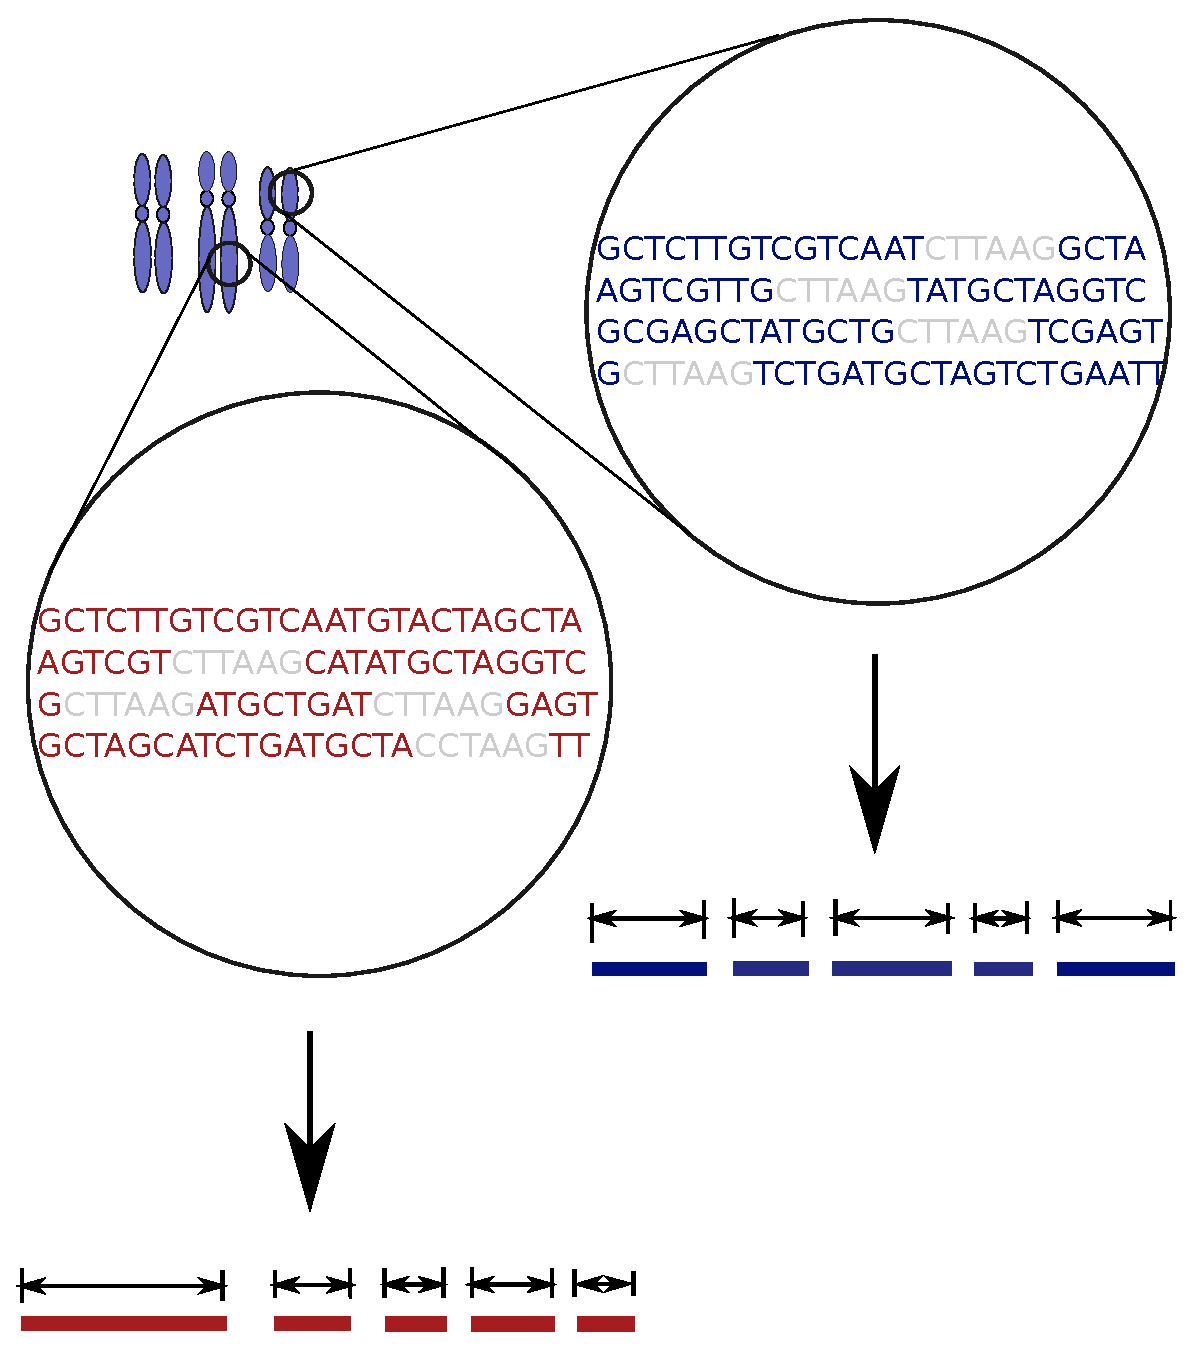
\includegraphics[width=0.35\textwidth]{./research_exam/slides/ormpub.eps}
   \label{figure:fig1}
 \end{SCfigure}



\paragraph{Our Contribution.}
We present the first index-based method for aligning contigs to an optical map.  
We call our tool $\twin$ to illustrate the association between the assembly and optical map as two representations of the genome sequence.  The first step of our procedure is to {\em in silico} digest the contigs with the set of restriction enzymes, computationally mimicking how each restriction enzyme would cleave the short segment of DNA defined by the contig.  Thus, {\em in silico digested contigs} are miniature optical maps that can be aligned to the much longer (sometimes genome-wide) optical maps.  The objective is to search and align the {\em in silico} digested contigs to the correct location in the optical map. 
By using a suitably-constructed FM-Index data structure~\cite{fm2005} built on the optical map,  we show that alignments between contigs and optical maps can be computed in time that is faster 
than competing methods by more than two orders of magnitude.  


$\twin$ takes as input a set of contigs and an optical map, and produces a set of alignments.  The alignments are output in Pattern Space Layout (PSL) format, allowing them to be visualized using any PSL visualization software, such as IGV~\cite{igv}.  $\twin$ is specifically designed to work on a wide range of genomes, anything from relatively small genomes, to large eukaryote genomes.  Thus, we demonstrate the effectiveness of $\twin$ on {\em Yersinia kristensenii}, rice, and budgerigar genomes.  Rice and budgerigar have genomes of total sizes 430 Mb and 1.2 Gb, respectively. {\em Yersinia kristensenii}, a bacteria with genome size of 4.6 Mb, is the smallest genome we considered.   Short read sequence data was assembled for these genomes, and the resulting contigs were aligned to the respective optical map.   We compared the performance of our tool with available competing methods; specifically, the method of Valouev et al.~\cite{Valouev06} and SOMA~\cite{Nagarajan08}.  $\twin$ has superior performance on all datasets, and is demonstrated to be the only current method that is capable of completing the alignment for the budgerigar genome in a reasonable amount of CPU time; SOMA~\cite{Nagarajan08} required over 77 days of machine time to solve this problem, whereas, $\twin$ required just 35 minutes. Lastly, we verify our approach on simulated {\em E. coli} data by showing our alignment method found correct placements for the {\em in silico} digested contigs on a simulated optical map.     $\twin$ is available for download at \url{http://www.cs.colostate.edu/twin}. 

\paragraph{Roadmap.}
We review related tools for the problem in the remainder of this section. Section~\ref{sec-background} 
then sets notation and formally lays the data structural tools we make use of. 
Section~\ref{sec-methods} gives details of our approach. We report our experimental results in 
Section~\ref{sec-results}. Finally, Section~\ref{sec-discussion} offers reflections and some potentially 
fruitful avenues future work may take.

\paragraph{Related Work.}
The most recent tools to make use of optical mapping data in the context of assembly are AGORA~\cite{agora} and SOMA~\cite{Nagarajan08}. AGORA~\cite{agora} uses the optical map information to constrain de Bruijn graph construction with the aim of improving the resulting assembly. SOMA~\cite{Nagarajan08} is a scaffolding method that uses an optical map and is specifically designed for short-read assemblies. SOMA requires an alignment method for scaffolding and implements an $O(n^2 m^2)$-time dynamic programming algorithm. Gentig~\cite{Anantharaman01}, and software developed by Valouev et al.~\cite{Valouev06} also use dynamic programming to address the closely related task of finding alignments between optical maps. Gentig is not available for download.  BACop~\cite{Zhou09} also uses a dynamic programming algorithm and corresponding scoring scheme that gives more weight to contigs with higher fragment density. Antoniotti et al.~\cite{antoniotti} consider the unique problem of validating an optical map by using assembled contigs. This method assumes the contigs are error-free. Optical mapping data was produced for Assemblathon 2~\cite{bradnam2013assemblathon}.














 
\makeatletter{}\section{Background}
\label{sec-background}

\paragraph{Strings.}
Throughout we consider a string $\X = \X[1..n] = \X[1]\X[2]\ldots
\X[n]$ of $|\X| = n$ symbols drawn from the alphabet $[0..\sigma-1]$.
For $i=1,\ldots,n$ we
write $\X[i..n]$ to denote the {\em suffix} of $\X$ of length $n-i+1$,
that is $\X[i..n] = \X[i]\X[i+1]\ldots \X[n]$.  
Similarly, we write
$\X[1..i]$ to denote the {\em prefix} of $\X$ of length $i$.
$\X[i..j]$ is the {\em substring} $\X[i]\X[i+1]\ldots \X[j]$ of $\X$
that starts at position $i$ and ends at $j$. 

\paragraph{Optical Mapping.}
From a computational point of view, optical mapping is a process that takes two
strings: a genome $\A[1,n]$ and a restriction sequence $\B[1,b]$, and produces
an array (string) of integers $\M[1,m]$, such that $\M[i] = j$ if and only if 
$\A[j..j+b] = \B$ is the $i$th occurrence of $\B$ in $\A$.

For example, if we let $\B = \mbox{{\em act}}$ and 

\begin{center}
\begin{tabular}{p{0.4cm}*{22}{p{0.4cm}}}
& $\scriptstyle 1 $& $\scriptstyle 2 $& $\scriptstyle 3$& $\scriptstyle 4 $& $\scriptstyle 5 $& 
$\scriptstyle 6 $& $\scriptstyle 7 $& $\scriptstyle 8 $& $\scriptstyle 9 $& $\scriptstyle 10$&
$\scriptstyle 11 $& $\scriptstyle 12 $& $\scriptstyle 13$& $\scriptstyle 14 $& $\scriptstyle 15 $& 
$\scriptstyle 16 $& $\scriptstyle 17 $& $\scriptstyle 18 $& $\scriptstyle 19 $& $\scriptstyle 20$&
$\scriptstyle 21 $& $\scriptstyle 22 $\\
$\A $& $a$ & $t$ & $a$ & $c$ & $t$ & $t$ & $a$ & $c$ & $t$ & $g$ & $g$ 
&      $a$ & $c$ & $t$ & $a$ & $c$ & $t$ & $a$ & $a$ & $a$ & $c$ & $t$ \\
\end{tabular}
\end{center}

then we would have 
$$\M = 3,7,12,15,20.$$

It will also be convenient to view $\M$ slightly differently, as an array of fragment 
sizes, or distances between occurrences of $\B$ in $\A$ (equivalently differences
between adjacent values in $\M$). We denote this {\em fragment size domain} of $\M$, 
as the array $\F[1,m]$, defined such that $\F[i] = (\M[i]-\M[i-1])$, with $\F[1] = \M[1]-1$.  
Continuing with the example above, we have

$$\F = 2,4,5,3,5.$$


\paragraph{Suffix Arrays.}
The suffix array~\cite{mm1993} $\SA_{\X}$ (we drop subscripts when
they are clear
from the context) of a string $\X$
is an array $\SA[1..n]$ which
contains a permutation of the integers $[1..n]$ such that $\X[\SA[1]..n]
< \X[\SA[2]..n] < \cdots < \X[\SA[n]..n]$.  In other words, $\SA[j] =
i$ iff $\X[i..n]$ is the $j^{\mbox{{\scriptsize th}}}$ suffix of $\X$
in lexicographical order.

\paragraph{SA Intervals.} 
For a string $\Y$, the $\Y$-interval in the suffix array $\SA_{\X}$ is
the interval $\SA[s..e]$ that contains all suffixes having $\Y$ as a
prefix. The $\Y$-interval is a representation of the occurrences of
$\Y$ in $\X$. For a character $c$ and a string $\Y$, the computation
of $c\Y$-interval from $\Y$-interval is called a \emph{left extension}.

\paragraph{BWT and backward search.}
The Burrows-Wheeler Transform~\cite{bw1994} $\BWT[1..n]$ is a
permutation of $\X$ such that $\BWT[i] = \X[\SA[i]-1]$ if $\SA[i]>1$
and $\$$ otherwise. We also define $\LF[i] = j$ iff $\SA[j] =
\SA[i]-1$, except when $\SA[i] = 1$, in which case $\LF[i] = I$,
where $\SA[I] = n$.

Ferragina and Manzini~\cite{fm2005} linked $\BWT$ and $\SA$ in the
following way.  
Let $\C[c]$, for symbol $c$, be the number of symbols
in $\X$ lexicographically smaller than $c$.  The function
$\rank(\X,c,i)$, for string $\X$, symbol $c$, and integer $i$, returns
the number of occurrences of $c$ in $\X[1..i]$.  It is well known that
$\LF[i] = \C[\BWT[i]] + \rank(\BWT,\BWT[i],i)$.  Furthermore, we can
compute the left extension using $\C$ and $\rank$.  If $\SA[s..e]$ is
the $\Y$-interval,
then
$\SA[\C[c]+\rank(\BWT,c,s),\C[c]+\rank(\BWT,c,e)]$ is
the $c\Y$-interval.
This is called \emph{backward search}~\cite{fm2005}, and a data
structure supporting it is called an {\em FM-index}.

 
\makeatletter{}
\section{Methods}
\label{sec-methods}



We find alignments in four steps.  First, we convert contigs from the sequence domain to the optical map domain through the process of {\em in silico} digestion. Second, an FM-index is built from the sequence of optical map fragment sizes. Third, we execute a modified version of the FM-index backward search algorithm described in Section~\ref{sec-background} that allows inexact matches.
As a result of allowing inexact matches, there may be multiple fragments in an optical map that could each be a reasonable match for an {\em in silico} digested fragment, and in order to include all of these as candidate matches, backtracking becomes necessary in the backward search.
For every backward search path that maintains a non-empty interval for the entire query contig, we emit the alignments denoted by the final interval.

\subsection{Converting Contigs to the Optical Map Domain}

In order to find alignments for contigs relative to the optical map, we must first convert the strings of bases into the domain of optical maps, that is, strings of fragment sizes.
We do this by performing an {\em in silico} digest of each contig, which is performing a linear search over its bases, searching for occurrences of the enzyme recognition sequence and then computing the distances between adjacent restriction sites. 
These distances are taken to be equivalent to the fragment sizes that would result if the contig's genomic region underwent digestion in a lab.  
Additionally, the end fragments of the {\em in silico} digested contig are removed, as the outside ends are most likely not a result of the optical map restriction enzyme digestion, but rather an artifact of the sequencing and assembly process.


\subsection{Building an FM-index from Optical Mapping Data}
\label{subsec-buildfm}



We construct the FM-index for $\ell$, the string of 
fragment sizes. 
The particular FM-index implementation we use is the SDSL-Lite\footnote{\url{https://github.com/simongog/sdsl-lite}.} \cite{SDSL}
library's \emph{compressed suffix array with integer wavelet tree} data structure\footnote{The exact revision we used was commit ae42592099707bc59cd1e74997e635324b210115.}.


In preparation for finding alignments, we also keep two auxiliary data structures. The first is the suffix array, $\SA_{\scriptsize \F}$, corresponding to our FM-index, which we use to report the positions in $\ell$ where alignments of a contig occur. While we could decode the relevant entries of $\SA$ on demand with the FM-index in $O(p)$ time, where $p$ is the so-called sample period of the FM-index, storing $\SA$ explicitly significantly improves runtime at the cost of a modest increase in memory usage. The second data structure we store is $\M$, which allows us to map from positions in $\ell$ to positions in the original genome in constant time.

\subsection{Alignment of Contigs Using the FM-index}
After constructing the FM-index of the optical map, we find alignments between the optical map and the {\em in silico} digested contigs.  


Specifically, we try to find substrings of the optical map fragment sequence $\ell$ that are similar to the string of each {\em in silico} digested contig's non-end fragments $F$ satisfying an alignment goodness metric suggested by Nagarajan et al. \cite{Nagarajan08} \footnote{N.B. Alternative goodness metrics could be substituted.  They must satisfy the property that pairs of strings considered to align well are composed of substrings that are also considered to align well would also work.}:
\begin{displaymath}
\Bigl \lvert \sum_{i=s}^{t}F_i - \sum_{j=u}^{v}\ell_j \Bigr \rvert \le F_\sigma \sqrt{\sum_{j=u}^{v}\sigma_{j}^{2}},
\end{displaymath}
where a parameter $F_\sigma$  will affect the precision/recall tradeoff.


This computation is carried out using a modified FM-index backward search.  
A simplified, recursive version of our algorithm for finding alignments is shown in Algorithm \ref{match}.
The original FM-index backward search proceeds by finding a succession of intervals in the suffix array of the original text that progressively match longer and longer suffixes of the query string, starting from the rightmost symbol of the query.   Each additional symbol in the query string is matched in a process taking two arguments: 1) a suffix array interval, the $\Y$-interval, corresponding to the suffixes in the text, $\ell$, whose prefix matches a suffix of the query string, and 2) an extension symbol $c$.  The process returns a new interval, the $c\Y$-interval, where a prefix of each text suffix corresponding to the new interval is a left extension of the previous query suffix. This process is preserved in $\twin$, and is represented by the function \emph{BackwardSearchOneSymbol} in the $\twin$ algorithm, displayed in Algorithm~\ref{match}.


Since the optical map fragments include error from the measurement process, 
it cannot be assumed an {\em in silico} fragment size will exactly match the optical map fragment size from the same locus in the genome.
To accomodate these differences, we determine a set of distinct candidate match fragment sizes, $D$, each similar in size to the next fragment to be matched in our query. These candidates are drawn from the 
 interval of the BWT currently active in our backward search.
We do this by a wavelet tree traversal function provided by SDSL-Lite, which implements the algorithm described in~\cite{GNPtcs11} and takes $O(|D|\log(f/\Delta))$ time. This is represented by the function \emph{RestrictedUniqueRangeValues} in Algorithm~\ref{match}. We emphasise that, due to the large alphabet of $\ell $, the wavelet tree's ability to list unique values in a range efficiently is vital to overall performance. Unlike in other applications where the FM-index is used for approximate pattern matching (e.g. read alignment), we cannot afford a bruteforce enumeration of the alphabet at each step in the backward search.

These candidates are chosen to be within a reasonable noise tolerance, $t$, based on assumptions about the distribution of optical measurement error around the true fragment length.
 Since there may be multiple match candidates in the BWT interval of the optical map for a query fragment, we extend the backward search with backtracking so each candidate size computed from the wavelet tree is evaluated.  That is, for a given {\em in silico} fragment size (i.e. symbol) $c$, every possible candidate fragment size, $c'$, that can be found in the optical map in the range $c - t \ldots c + t$ and in the interval $s \ldots e$ (of the BWT) for some tolerance $t$ is used as a substitute in the backward search. Each of these candidates is then checked to ensure that a left extension would still satify the goodness metric, and then used as the extension symbol in the backward search.  So it is actually a set of $c'\Y$-intervals that is computed as the left extension in $\twin$.  Additionally, small DNA fragments may not adhere sufficiently to the glass surface and can be lost in the optical mapping process, so we also branch the backtracking search both with and without small {\em in silico} fragments to accomodate the uncertainty.

Each time the backward search algorithm successfully progresses throughout the entire query (i.e. it finds some approximate match in the optical map for each fragment in the contig query), we take the contents of the resulting interval in the $\SA$ as representing a set of likely alignments.










\renewcommand{\algorithmiccomment}[1]{\hskip0em$\triangleright$ #1}

\begin{algorithm}[t]
\caption{{\sc Match}($s$, $e$, $q$, $h$) Provided a suffix array start index $s$ and end index $e$, query string $q$, and rightmost unmatched query string index $h$ (initially $s=1$, $e=m$, $h=|q| - 1$), emit alignments of an \emph{in silico} digested contig to an optical map.}
\label{match}
\begin{algorithmic}

\Procedure{Match}{$s$,$e$,$q$,$h$}
\If{$h = -1$} 
  \State \Comment{Recursion base case.  Suffix array indexes $s .. e$ denote original query matches.}
  \State{ \emph{Emit}$(s, e)$} 
\Else
  \State \Comment{The next symbol to match, $c$, is the last symbol in the query string.}
  \State $c \leftarrow q[h]$ 
  \State \Comment{Find the approximately matching values in $\BWT[s \ldots e]$, within tolerance $t$.}
  \State $D \leftarrow$ \emph{RestrictedUniqueRangeValues}(s, e, $c + t$, $c - t$) 
  \State \Comment{Let $c'$ be one possible substitute for $c$ drawn from $D$}
  \ForAll{$c' \in D$} 
    \State \Comment{If Equation 1 is still satisified with $c' $ and $c$, ...}
    \If{ $\Bigl \lvert \sum_{i=0}^{|q|-h}\SA[s]_i + c' - \sum_{j=h}^{|q|-1}q_j - c \Bigr \rvert \le F_\sigma \sqrt{\sum_{j=0}^{|q|-h}\sigma_{j}^{2}}$
    } 
    \State \Comment{... determine the suffix array range of the left extension of $c'$.}
    \State $s', e' \leftarrow$ \emph{BackwardSearchOneSymbol}($s,e,c'$) 
      \State \Comment{Recurse to attempt to match the currently unmatched prefix.}
      \State {\sc Match}($s', e', q, h - 1$) 
    \EndIf
  \EndFor
\EndIf
\EndProcedure
\end{algorithmic}
\end{algorithm}


   
\subsection{Output of Alignments in PSL format}
For each {\em in silico} digested contig that has an approximate match in the optical map, we emit the alignment, converting positions in the fragment string $\ell$ to positions in the genome using the $\M$ table. We provide a script to convert the human readable output into PSL format.  
\makeatletter{}\section{Results}\label{sec-results}

We evaluated the performance of $\twin$ against the best competing methods on \emph{Yersinia kristensenii}, rice and budgerigar.  These three genomes were chosen because they have available sequence and optical mapping data and are diverse in size.   For each dataset, we compared the runtime, peak memory usage, and the number of contigs for which at least one alignment was found for $\twin$, SOMA~\cite{Nagarajan08}, and the software of Valouev et al.~\cite{Valouev06}.  Peak memory was measured as the maximum resident set size as reported by the operating system.  Runtime is the user process time, also reported by the operating system.   SOMA~\cite{Nagarajan08} v2.0 was run with example parameters provided with the tool and the software of Valouev et al.~\cite{Valouev06} was run with its scoring parameters object constructed with arguments (0.2, 2, 1, 5, 17.43, 0.579, 0.005, 0.999, 3, 1). $\twin $ was run with $D_\sigma = 4$, $t = 1000$, and $[250 \ldots 1000]$ for the range of small fragments.
Gentig~\cite{Anantharaman01} and BACop~\cite{Zhou09} were not available for download so we did not test the data using these approaches.      
  
The sequence data was assembled for  \emph{Yersinia kristensenii}, rice and budgerigar by using various assemblers. 
The relevant assembly statistics are given in Table~\ref{tab:assembly_stats}.  An important statistic in this table is the number of contigs that have at least two restriction sites, since contigs with fewer than two are unable to be aligned meaningfully by any method, including $\twin$.  This statistic was computed to reveal cases of ambiguity in placement from lack of information. Indeed, Assemblathon~2 required there to be nine restriction sites present in a contig to align it to the optical mapping data \cite{bradnam2013assemblathon}.  All experiments were performed on Intel x86-64 workstations with sufficient RAM to avoid paging, running  64-bit Linux.

The experiments for \emph{Yersinia kristensenii}, rice and budgerigar illustrate how each of the programs' running time scale as the size of the genome increases.  However, due to the possibility of mis-assemblies in these draft genomes, comparing the actual alignments could possibly lead to erroneous conclusions.  Therefore, we will verify the alignments using simulated {\em E. coli} data.  See Subsection \ref{sec:ecoli} for this experiment.  


\makeatletter{}\begin{table*}
\centering
\begin{tabular}{| p{0.20\linewidth} |  
			  p{0.15\linewidth} | 
			  p{0.15\linewidth} | 
			  p{0.45\linewidth} |}
\hline
Genome                     		 			 	& N50   	& Genome Size 		& No. of Contigs with  $\geq$ 2 restriction sties\\
	                     		   		  		
\hline
{\em Y. kristensenii}     	 		         & 30,719 	& 4.6 Mb 				& 92 \\
Rice                       		 		         	& 5,299  	& 430 Mb 				& 3,103 \\
Budgerigar                     	         			         	& 77,556 	& 1.2 Gb 				& 10,019 \\
\hline
\end{tabular}
\caption{Assembly and genome statistics for \emph{Yersinia kristensenii}, rice and budgerigar.  The assembly statistics were obtained from Quast. \cite{QUAST}.}
\label{tab:assembly_stats}
\end{table*} 

\subsection{Performance on \emph{Yersinia kristensenii}} \label{sec:pro_genome}

The sequence and optical map data for  \emph{Yersinia kristensenii} are described by Nagarajan {\em et al.} \cite{Nagarajan08}.  The \emph{Yersinia kristensenii} ATCC 33638 reads were generated using 454 GS 20 sequencing and assembled using SPAdes version 3.0.0 \cite{spades} using default parameters.   Contigs from this assembly were aligned against an optical map of the bacterial strain generated by OpGen using the AfIII restriction enzyme.  There are approximately 1.4 million single-end reads for this dataset, and they were obtained from the NCBI Short Read Archive (accession SRX013205).  Of the 92 contigs that could be aligned to the optical map, the software of  Valouev et al. aligned 91 contigs, SOMA aligned 54 contigs, and $\twin$ aligned 61 contigs.  Thus, $\twin$ found more alignments than SOMA, and did so faster. It should be noted that, for this dataset, all three tools had reasonable runtimes. However, while the software of Valouev et al. found more alignments, our validation experiments (below) suggest these results may favor recall over precision, and many of the additional alignments may not be credibled.  


\subsection{Performance on Rice Genome} \label{section:rice}

The second dataset consists of approximately 134 million 76 bp paired-end reads from {\em Oryza sativa Japonica} rice, generated by Illumina, Inc. on the Genome Analayzer (GA) IIx platform, as described by Kawahara {\em et al.} \cite{kawahara2013improvement}.   These reads were obtained from the NCBI Short Read Archive (accession SRX032913) and assembled using SPAdes version 3.0.0 \cite{spades} using default parameters.  The optical map for rice was constructed by Zhou {\em et al.} \cite{RICE} using SwaI as the restriction enzyme.  This optical map was assembled from single molecule restriction maps into 14 optical map contigs, labeled as 12 chromosomes, with chromosome labels 6 and 11 both containing two optical map contigs.

Again, $\twin$ found alignments for more contigs than SOMA on the rice genome.  SOMA and $\twin$ found alignments for 2,434, and 3,098 contigs, respectively, out of 3,103 contigs that could be aligned to the optical map.  However, while SOMA required over 29 minutes to run, $\twin$ required less than one minute. 
The software of Valouev executed faster than SOMA (taking around 3 minutes), though still several times slower than $\twin$ on this modest sized genome.


\subsection{Performance on Budgerigar Genome} \label{section:parrot}

The sequence and optical map data for the budgerigar genome were generated for the Assemblathon~2 project of Bradnam {\em et al.} \cite{bradnam2013assemblathon}.   Sequence data consists of  a combination of Roche 454, Illumina, and Pacific Biosciences reads, providing 16x, 285x, and 10x coverage (respectively) of the genome.  All sequence reads are available at the NCBI Short Read Archive (accession  ERP002324).  For our analysis we consider the assembly generated using Celera~\cite{celera}, which was completed by the CBCB team (Koren and Phillippy) as part of  Assemblathon 2~\cite{bradnam2013assemblathon}.  The optical mapping data was created by Zhou, Goldstein, Place, Schwartz, and Bechner using the SwaI restriction enzyme and consists of 92 separate pieces. 
As with the two previous data sets, $\twin$ found alignments for more contigs than SOMA on the budgerigar genome.  SOMA and $\twin$ found alignments for 9,668, and 9,826 contigs, respectively, out of 10,019 contigs that could be aligned to the optical map.  However,  SOMA required over 77 days of CPU time and $\twin$ required 35 minutes.  The software of Valouev et al. returned 9,814 alignments and required over an order of magnitude (6.5 hours) of CPU time.  Hence, $\twin$ was the only method that efficiently aligned the {\em in silico} digested budgerigar genome contigs to the optical map.  It should be kept in mind that the competing methods were developed for prokaryote genomes and so we are repurposing them at a scale for which they were not designed.   Lastly, the amount of memory used by all the methods on all experiments was low enough for them to run on a standard workstation.  

We were forced to parallelize SOMA due to the enormous amount of CPU time SOMA required for this dataset.  To accomplish this task, the FASTA file containing the contigs was split into 300 different files, and then IPython Parallel library was used to invoke up to two instances of SOMA on each machine from a set of 150 machines.  Thus, when using a cluster with up to 300 jobs concurrently, the alignment for the budgerigar genome took about a day of wall clock time. In contrast, we ran the software of Valouev et al. and $\twin$ with a single thread running on a single core.  However, it should be noted that the same parallelization could have been accomplished for both these software methods too. Also, even with parallelization of SOMA, $\twin$ is still an order of magnitude faster than it.


\makeatletter{}
\begin{table*}[t]
\centering

\begin{tabular}{| 
			p {0.22\linewidth} |
			p {0.20\linewidth} |
			p {0.15\linewidth} |
			p {0.13\linewidth} |
			p {0.25\linewidth} | }
			
			\hline
{\bf Genome} 			&  {\bf Program}	& {\bf Memory }	& {\bf Time } 			& {\bf Aligned Contigs} \\ 

\hline
\hline
{\em Y. Kristensenii} & & &  & \\
\hline

				& Valouev {\em et al.} 	& 1.81 		& .17 s 			& 91  \\
				& SOMA 				& 1.71 		& 7.32 s 			& 54 \\
				& $\twin$
                                & 18  		& .06 s
                                & 65\\
\hline
\hline
Rice & & &   & \\
\hline 

				& Valouev {\em et al.} 	& 11.25 		& 2 m 57 s 			& 2,676  \\
				& SOMA 				& 7.94 		& 29 m 38 s 		& 2,434 \\
				& $\twin$
                                & 18.25  		&  50 s 			&  3,098\\
\hline
\hline
Budgerigar & & & & \\
\hline 

				& Valouev {\em et al.} 	& 390  			& 6.5 h 		& 9,814 \\
				& SOMA 				& 380.95  		& 77.2 d 		& 9,668 \\
				& $\twin$                         &127.112                  &  35 m           & 9,826\\

\hline
\end{tabular}
\caption{{\bf Comparsion of the alignment results for $\twin$ and competing method.}  The performance of $\twin$ was compared against SOMA \cite{Nagarajan08} and the method of Valouev et al.~\cite{Valouev06} using the assembly and optical mapping data for {\em Yersinia Kristensenii}, rice, and budgerigar.  Various assemblers were used to assemble the data for these species.  The relevant statistics and information concerning these assemblies and genomes can be found in Table \ref{tab:assembly_stats}.  The peak memory is given in megabytes (mb).  The running time is reported in seconds (s), minutes (m), hours (h), and days. }
\label{tab:possible_columns}
\end{table*} 

 

\subsection{Alignment Verification} \label{sec:ecoli}

We compared the alignments given by $\twin$ against the alignments of the contigs of an {\em E. coli} assembly to the \emph{E. Coli} (str. K-12 substr. MG1655) reference genome.  Our prior experiments involved species for which the reference genome may have regions that are mis-asssembled and therefore, contig alignments to the reference genome may be inaccurate and cannot be used for comparison and verification of the {\em in silico} digested contig alignment.   The {\em E. coli} reference genome is likely to contain the fewest errors and thus, is the one we used for assembly verification.  The sequence data consists of approximately 27 million paired-end 100 bp reads from {\em E. coli} (str. K-12 substr. MG1655) generated by Illumina, Inc. on the Genome Analayzer (GA) IIx platform, and  was obtained from the NCBI Short Read Archive (accession ERA000206), and was assembled using SPAdes version 3.0.0 \cite{spades} using default parameters.  This assembly consists of 160 contigs; 50 of which contain two restriction sites, the minimum required for any possible optical alignment, and complete alignments with minimal (\textless 800 bp) total in/dels relative to the reference genome.

We simulated an optical map using the reference genome for {\em E. coli} (str. K-12 substr. MG1655) since there is no publicly available one for this genome.  

The 50 contigs that contained more than two restriction sites were aligned to the reference genome using BLAT~\cite{blat}.  These same contigs were then {\em in silico} digested and aligned to the optical map using $\twin$.  The resulting PSL files were then compared.  $\twin$ found alignment positions within 10\% of those found by BLAT for all 50 contigs, justifying that our method is finding correct alignments.  We repeated this verification approach with both SOMA and the software from Valouev.  All of SOMA's reported alignments had matching BLAT alignments, while of the 49 alignments the software from Valuoev reported, only 18 could be matched with alignments from BLAT.
 
\makeatletter{}\section{Discussion and Conclusions}
\label{sec-discussion}

We demonstrated that $\twin$, an index-based algorithm for aligning {\em in silico} digested contigs to an optical map, gave over an order of magnitude improvement to runtime without sacrificing alignment quality. Our results show that we are able to handle genomes at least as large as the budgerigar genome directly, whereas SOMA cannot feasibly complete the alignment for this genome in a reasonable amount of time without significant parallelization, and even then is orders of magnitude slower than $\twin$. Indeed, given its performance on the budgerigar genome, and its $O(m^2 n^2)$ time complexity, larger genomes seem beyond SOMA.  For example, the loblolly pine tree genome, which is approximately 20 Gb \cite{pinetree}, would take SOMA approximately 84 machine years, which, even with parallelization, is prohibitively long.

Lastly, optical mapping is a relatively new technology, and thus, with so few algorithms available for working with this data, we feel there remains good opportunities for developing more efficient and flexible methods. Dynamic programming optical map alignment approaches are still important today, as the assembly of the consensus optical maps from the individually imaged molecules often has to deal with missing or spurious restriction sites in the single molecule maps when enzymes fail to digest a recognition sequence or the molecule breaks.  Though coverage is high (e.g. about 1,241 Gb of optical data was collected for the 2.66 Gb goat genome), there may be cases where missing restriction site errors are not resolved by the assembly process.   In these rare cases (only 1\% of alignments reported by SOMA on parrot contain such errors) they will inhibit $\twin$'s ability to find correct alignments.  In essence, $\twin$ is trading a small degree of sensitivity for a huge speed increase, just as other index based aligners have done for sequence data.  Sir\'{e}n et al.~\cite{dag_method} recently extended the Burrows-Wheeler transform (BWT) from strings to acyclic directed labeled graphs and to support path queries. In future work, an adaptation of this method for optical map alignment may allow for the efficient handling of missing or spurious restriction sites.

 
\makeatletter{} \section{Conclusion}
















 

\section{Misassembly Detection using Paired-End Sequence Reads \\ and Optical Mapping Data}
In this section, we explore how faster alignment of TWIN enables better assembly validatio.

\makeatletter{}\begin{abstract} 
A crucial problem in genome assembly is the discovery and correction of misassembly errors in draft genomes.  
We develop a method that will enhance the quality of draft genomes by identifying and removing misassembly errors using paired short read sequence data and optical mapping data.  
We apply our method to various assemblies of the loblolly pine and {\em Francisella tularensis} genomes.  
Our results demonstrate that we detect more than 54\% of extensively misassembled contigs and more than 60\% of locally misassembed contigs in an assembly of {\em Francisella tularensis}, and between 31\% and 100\% of extensively misassembled contigs and between 57\% and 73 \% of locally misassembed contigs in the assemblies of loblolly pine.  
$\sequel$ can be downloaded at \url{http://www.cs.colostate.edu/seq/}.
\end{abstract}
 


\makeatletter{}\subsection{Introduction} \label{sec:intro}
Comparing genetic variation between and within a species is a fundamental activity in biological research. For example,  there is currently a major effort to sequence entire genomes of agriculturally important plant species to identify parts of the genome variable in a given breeding program and, ultimately, create superior plant varieties. Robust genome assembly methods are imperative to these large sequencing initiatives and other scientific projects~\cite{haussler2008genome,robinson2011creating,1001_arabidopsis,hmp} because scientific analyses frequently use those genomes to determine genetic variation and associated biological traits. 

At present, the majority of assembly programs are based on the Eulerian assembly paradigm~\cite{IW95,PTW}, where a de Bruijn graph is constructed with a vertex $v$ for every $(k - 1)$-mer present in a set of reads, and an edge $(v, v')$ for every observed $k$-mer in the reads with $(k - 1)$-mer prefix $v$ and $(k - 1)$-mer suffix $v'$. A contig corresponds to a non-branching path through this graph. We refer the reader to Compeau et al.~\cite{compeau} for a more thorough explanation of de Bruijn graphs and their use in assembly.  The assemblers Euler-SR \cite{Chaisson:2008}, Velvet \cite{Zerbino:2008}, SOAPdenovo \cite{soap}, ABySS \cite{Simpson:2009} and ALLPATHS \cite{Butler:2008} all use this paradigm and follow the same general outline: extract $k$-mers from the reads, construct a de Bruijn graph from the set $k$-mers, simplify the graph, and construct contigs.  

One crucial problem that persists in Eulerian assembly (and genome assembly, in general) is the discovery and correction of misassembly errors in draft genomes.  
We define a {\em misassembly error} as an assembled region that contains a significantly large insertion, deletion, inversion, or rearrangment that is the result of decisions made by the assembly program.  Identification of misassembly errors is important because true biological variations manifest in similar ways and thus, these errors can be easily misconstrued as true genetic variation~\cite{salzberg}. This can mislead a range of genomic analyses.  
We note that the exact definition of a misassembly error can vary, and adopt the standard definition used by Quast~\cite{quast} and other tools.  See section \ref{subsec:data} for this exact definition.  
Once the existence and 
location of a misassembly 
is identified, 
it
can be removed by segmenting the contig at that location.

   

We present a computational method for identifying misassembly errors using a combination of short reads and optical mapping data.   Optical mapping is a system developed in 1993~\cite{schwartz93} that can construct ordered, genome-wide, high-resolution restriction maps.  The system works as follows \cite{ORMenc,microfluidic}: an ensemble of DNA molecules adhered to a charged glass plate are elongated by fluid flow.   An enzyme is then used to cleave them into fragments at loci where the corresponding recognition sequence occurs. Next, the fragments are highlighted with fluorescent dye and imaged under a microscope. Finally, these images are analyzed to estimate the fragment sizes, producing a molecular map. Since the fragments stay relatively stationary during the aforementioned process, the images capture their relative order and size~\cite{Neely11}.   Multiple copies of the genome undergo this process, and a consensus map is formed that consists of an ordered sequence of fragment sizes, each indicating the approximate number of bases between occurrences of the recognition sequence in the genome \cite{Anantharaman01}.  

Although optical mapping data has been used for discerning structural variation in the human genome  \cite{teague}, and for scaffolding and validating contigs for several large sequencing projects --- including those for various prokaryote species \cite{reslewic,zhou,zhou2}, rice~\cite{RICE}, maize \cite{Zhou09}, mouse \cite{church}, goat~\cite{GOAT}, parrot~\cite{gigadb}, and {\em Amborella trichopoda} \cite{amborella} --- there exists no publicly available tools for using this data for misassembly correction using short read and optical mapping data.

Our tool, which we call $\sequel$, predicts which contigs are misassembled and the approximate locations of the errors in the contigs.  It takes as input the paired-end sequence read data, contigs, an ensemble of optical maps, and the restriction enzymes used to construct the optical maps.
$\sequel$ first uses the paired-end read data to divide the contigs into two sets: those that are predicted to be correctly assembled and those that are not.  
Then the set of  contigs that are candidates for containing misassembly errors are further divided into misassembled contigs and correctly assembled contigs using optical mapping data.
Fundamental to the first step is the concept of a {\em red-black positional de Bruijn graph}, which encapsulates recurring artifacts in the alignment of the sequence read data to the contigs and their position in the contig. 
The red vertices in this graph indicate if a contig is likely to be misassembled and also flag the location where the misassembly error occurs. These locations are called {\em  misassembly breakpoints}.

In the second stage of $\sequel$ where optical mapping data is used, the contigs conjectured to be misassembled are {\em in silico} digested with the set of input restriction enzymes and aligned to the optical map using Twin~\cite{wabi2014}.  Based on the presence or absence of alignment, a prediction of misassembly is made.  The {\em in silico} digestion process computationally mimics how each restriction enzyme would cleave the segment of DNA defined by the contig, returning ``mini-optical maps'' that can be aligned to the optical map for the whole genome. An important aspect of our work is that it highlights the need to use another source of information, which is independent of the sequence data but representative of the same genome, in order to identify misassembly errors. We show that optical mapping data can be used as this information source.   
 

We give results for the {\em Francisella tularensis} and loblolly pine genomes.  Each genome was assembled using various de Bruijn graph assemblers and then misassembly errors were predicted.  Our results on {\em Francisella tularensis} show that $\sequel$ correctly identifies (on average) 86\% and 80\% of locally and extensively misassembled contigs, respectively. This is a considerable improvement on existing methods, which identified (on average)  26\% and 16\% of locally and extensively misassembled contigs, respectively, in the same assemblies. The results on the loblolly pine genome assemblies show similar improvement. Lastly, our results demonstrate we are capable of significantly decreasing the false positive rate in all assemblies of {\em Francisella tularensis} and loblolly pine by incorporating optical map data into the prediction; the reduction was between 29\% and 74\%.  

\paragraph{Related Work.}  
Both amosvalidate~\cite{amos} and REAPR~\cite{reapr} are capable of identifying and correcting misassembly errors.  
REAPR is designed to use both short insert and long insert paired-end sequencing libraries, however, it can operate with only one of these types of sequencing data.  
Amosvalidate, which is included as part of the AMOS assembly package~\cite{amos2}, was developed specifically for first generation sequencing libraries~\cite{amos}. 
iMetAMOS~\cite{iMetAMOS} is an automated assembly pipeline that provides error correction and validation of the assembly.  
It packages several open-source tools and provides annotated assemblies that result from an ensemble of tools and assemblers.  
Currently, it uses REAPR for misassembly error correction. 
 
Many optical mapping tools exist and deserve mentioning, including AGORA~\cite{agora}, SOMA~\cite{soma}, and Twin~\cite{wabi2014}. AGORA~\cite{agora} uses the optical map information to constrain de Bruijn graph construction with the aim of improving the resulting assembly.   SOMA~\cite{soma} uses dynamic programming to align {\em in silico} digested contigs to an optical map.   Twin~\cite{wabi2014} is an index-based method for aligning contigs to an optical map. Due to its use of an index data structure it is capable of aligning {\em in silico} digested contigs orders of magnitude faster than competing methods.     Xavier et al.~\cite{om_mis} demonstrated misassembly errors in bacterial genomes can be detected using proprietary software.

Lastly, there are special purpose tools that have some relation to $\sequel$ in their algorithmic approach.
Numerous assembly tools use a finishing process after assembly, including Hapsembler~\cite{Donmez2011}, LOCAS~\cite{LOCAS}, Meraculous~\cite{Chapman2011}, and the ``assisted assembly'' algorithm~\cite{Gnerre2009}. Hapsembler~\cite{Donmez2011} is a haplotype-specific genome assembly toolkit that is designed for genomes that are highly-polymorphic. Both RACA~\cite{raca}, and SCARPA~\cite{scarpa} perform paired-end alignment to the contigs as an initial step, and thus, are similar to our algorithm in that respect. 






 
\makeatletter{}\subsection{Methods}\label{sec-methods} 

$\sequel$ can be broken down into four main steps: recruitment of reads to contigs; construction of the red-black positional de Bruijn graph; misassembly error prediction; and misassembly verification using optical mapping data.   
We explain each of these steps in detail in the following subsections. 


        \begin{figure}[h!]
            \centering
              	\includegraphics[width=0.6\textwidth]{recomb15mis/types_of_misassemblies_read_alignment.pdf}
                	\caption{An illustration of the systematic alterations that occur with rearrangements and inversions.  (a) Shows the proper read alignment where mate-pair reads have the correct orientation and distance from each other. A  rearrangement or	inversion will present itself by the orientation of the reads being incorrect, and/or the distance of the mate-pairs being significantly smaller or larger than the expected insert size. This is shown in (b) and (c), respectively.}
                	\label{fig:read_alignment_1}
        \end{figure}
             	\begin{figure}[h!]
		\centering
                	\includegraphics[width=0.6\textwidth]{recomb15mis/types_of_misassemblies_read_alignment_2.pdf}
       		\caption{An illustration of the systematic alterations that occur with collapsed or expanded repeats.  (a) Shows the proper read depth, which is uniform across the genome. A collapsed or expanded repeat will manifest as significantly lower or higher read depth; (b) shows a collapsed repeat, where the read depth being significantly greater than expected; and (c) shows a expanded repeat, where the observed read depth is significantly lower than expected.}
        		\label{fig:read_alignment_2}
        \end{figure}


\subsection{Recruitment of Reads and Threshold Calculation}  

$\sequel$ first aligns reads to contigs in order to identify regions that contain abnormal read alignments.  
Collapsed or expanded repeats will present as the read coverage being greater or lower than the expected genome coverage in the region that has been misassembled.  Similarly, inversion and rearrangement errors will present as the alignment of the mate-pairs being rearranged. Figures \ref{fig:read_alignment_1} and \ref{fig:read_alignment_2} illustrate these unconventional read alignments. More specifically, this step consists of aligning all the (paired-end) reads to all the contigs and then calculating three thresholds, $\Delta_L$, $\Delta_U$ and $\Gamma$.  The range $[\Delta_L, \Delta_U]$ defines the acceptable read depth, and $\Gamma$ defines the maximum allowable number of reads whose mate-pair aligns in an unconventional manner (e.g. inverted orientation). 
In order to calculate these thresholds, we consider all alignments of each read as opposed to just the best alignment of each read since misassembly errors frequently occur within repetitive regions where the reads will align to multiple locations.  
$\sequel$ performs this step using BWA (version 0.5.9) in paired-end mode with default parameters \cite{bwa}.   Subsequently, after alignment, each contig is treated as a series of consecutive 200 bp regions.  These are sampled uniformly at random $\ell$ times, and the mean ($\mu_{d}$) and the standard deviation ($\sigma_d$) of the read depth and the mean ($\mu_{i}$) and the standard deviation ($\sigma_i$) of the number of alignments where an unconventional mate-pair orientation is witnessed are calculated from these sampled regions.   $\Delta_L$ is set to the maximum of $\{0, \mu_d - 3\sigma_d\}$, $\Delta_U$ is set to $\mu_d + 3\sigma_d$, and $\Gamma$ is set to $\mu_i + 3\sigma_i$.  The default for $\ell$ is $\frac{1}{20}$th of the contig length; this can be changed via an input parameter of $\sequel$.  



\subsection{Construction of the Red-Black Positional de Bruijn Graph} 


After threshold calculation, the red-black positional de Bruijn graph is constructed. For clarity, we begin by describing the {\em positional de Bruijn graph}, given by Ronen et al.~\cite{sequel}, and then define the red-black positional de Bruijn graph.  Whereas the edges in the traditional de Bruijn graph correspond to $k$-mers, the edges in the positional de Bruijn graph correspond to $k$-mers and their inferred positions on the contigs ({\em positional $k$-mers}).  Hence, the positional de Bruijn graph $G_{k, \Phi}$ is defined for a multiset of positional $k$-mers and parameter $\Phi$, and is constructed in a similar manner to the traditional de Bruijn graph using an A-Bruijn graph framework from \cite{PTT04}. Given a $k$-mer $s_k$, let $\prefix(s_k)$ be the first $k - 1$ nucleotides of $s_k$, and $\suffix(s_k)$ be the last $k - 1$ nucleotides of $s_k$.  Each positional $k$-mer $(s_k, p)$ in the input multiset corresponds to a directed edge in the graph between two positional $(k - 1)$-mers, $(\prefix(s_k), p)$ and $(\suffix(s_k), p + 1)$.  After all edges are formed, the graph undergoes a gluing operation. A pair of positional $(k - 1)$-mers, $(s_{k - 1}, p)$ and $(s_{k - 1}', p')$, are glued together into a single vertex if $s_{k - 1} = s_{k - 1}'$ and $p \in [p' - \Phi, p' + \Phi]$.  Two positional $(k - 1)$-mers are glued together if their sequences are the same and their positions are within $\Phi$ from each other. We refer to the {\em multiplicity} of a positional $(k - 1)$-mer $(s_{k - 1}, p)$ as the number of occurrences where $s_{k - 1}$ clustered at position $p$.  

$\sequel$ constructs the red-black positional de Bruijn graph from the alignment of the reads to the contigs. The red-black positional de Bruijn graph contains positional $k$-mers and is constructed in an identical way as the positional de Bruijn graph with the addition that each vertex ($(k - 1)$-mer) has an associated red or black color attributed to it that is defined using $\Delta_L$, $\Delta_U$ and $\Gamma$.  In addition to the multiplicity of each positional $(k - 1)$-mer, the number of positional $(k - 1)$-mers that originated from a read whose mate-pair did not align in the conventional direction is stored at each vertex.   When the multiplicity is less than $\Delta_L$ or greater than $\Delta_U$, or if the observed frequency of unconventional mate-pair orientation is greater than $\Gamma$, then the vertex is {\em red}; otherwise it is {\em black}.

\subsection{Misassembly Conjecture and Breakpoint Estimation}  

A red-black positional de Bruijn graph is constructed for each contig, and misassembly errors in each contig are detected by searching for consecutive red vertices in the corresponding graph.  Depth-first search is used for the graph traversal. If there are greater than 50 consecutive red vertices then the contig is conjectured to be misassembled.  The breakpoint in the contig can be determined by recovering the position of the corresponding red vertices (e.g., the positional $(k - 1)$-mers).  The number of consecutive red vertices needed to consider it misassembled can be changed via a command line parameter in $\sequel$.  Our experiments were performed with the default (e.g. 50), which corresponds to a region in the contig that has length $\geq$ 50 bp.  After this stage of the algorithm, we take contigs having regions exceeding that threshold as a set of contigs that are conjectured to be misassembled and their transitions in and out of those regions as breakpoints.

\subsection{Misassembly Verification} \label{dev}

Lastly, we use optical mapping data to verify whether a contig that is conjectured to be misassembled indeed is.  
Verification is based on the expectation that, after {\em in silico} digestion, a correctly assembled contig has a sequence of fragment sizes that is similar to that in the optical map at the corresponding locus in the genome.  In other words, an {\em in silico} digested contig should align to some region of the optical map since both are derived from the same region in the genome.
Conversely, since misassembled contigs are not faithful reconstructions of any part of the genome, when {\em in silico} digested, their sequence of fragments will likewise not have a corresponding locus in the optical map to which it aligns.  

Optical maps contain measurement error at each fragment size so some criteria is needed to decide whether variation in fragment size of an {\em in silico} digested contig and that of an optical map at a particular locus is due to variation in the size of the physical fragments or a consequence of optical measurement error.  
Due to this ambiguity, and the necessary tolerances to ensure correctly assembled contigs align to the locus in the optical map, misassembled contigs may also align to loci in the optical map, which by coincidence have a fragment sequence similar to the contig within the threshold margin of error.  
While there are various sophisticated approaches to determining statistical significance of an alignment, such as by Sakar et al.~\cite{statsigORMalign}, we use a $ \chi^2 $ model discussed by Nagarajan et al.~\cite{soma} and take the cumulative density function $\le$ 0.85 as evidence of alignment, which we found to work well empirically.

In addition, a misassembled contig only fails to align to the optical map if the enzyme recognition sequence, and thus the cleavage sites, exist in the contig in a manner that disrupts a good alignment (e.g. a misassembled contig with an inverted segment may still align if cleavage sites flank the inverted segment).
This implies that (a) some enzymes produce optical maps that have greater performance in identifying misassembly errors; and (b) alignment to the optical map is not as strong evidence for correct assembly as non-alignment to the optical map is for misassembly. 
This leads to the conclusion that an ensemble of optical maps (each made with a different enzyme) has a greater chance at revealing misassembly errors than a single optical map.  
Since acquiring three optical maps for one genome is reasonably accessible for many sequencing projects, the process of {\em in silico} digestion and alignment is repeated for three enzymes and the consensus of the alignment is taken over all of them, i.e., if two out of three times the contig did not align then it is deemed not to align (by the consensus).
A contig is deemed to be misassembled if it fails to align. The alignment is performed using Twin~\cite{wabi2014} (with default parameters) and then these results are filtered according to the $ \chi^2 $ model mentioned above.  
For our experiments, optical maps were simulated by {\em in silico} digesting reference genomes, adding normally distributed noise with a 150 bp standard deviation, and discarding fragments smaller than 700 bp.


                     
\makeatletter{}\subsection{Results} \label{sec:results} 

\subsection{Datasets} \label{subsec:data}

Our first dataset consists of approximately 6.9 million paired-end 101 bp reads from the prokaryote genome {\em Francisella tularensis}, generated by Illumina Genome Analayzer (GA) IIx platform. 
It was obtained from the NCBI Short Read Archive (accession number SRR063416). The reference genome was also downloaded from the NCBI website (Reference genome NC\_006570.2).  
The {\em  Francisella tularensis} genome is 1,892,775 bp in length. As a measure of quality assurance, we aligned the reads to the {\em Francisella tularensis} genome using BWA (version 0.5.9) \cite{bwa} with default parameters.  
We call a read {\em mapped} if BWA outputs an alignment for it and {\em unmapped} otherwise.  
Analysis of the alignments revealed that 97\% of the reads mapped to the reference genome, representing an average depth of approximately $367\times$.  

Our second dataset consists of approximately  31.3 million paired-end 100 bp reads from the loblolly pine  ({\em Pinus taeda} L.) genome~\cite{pine}.  
We downloaded the reference genome from the pine genome website~\cite{pinetreeweb} and simulated reads from the largest five hundred scaffolds from the reference using ART~\cite{art} (art illumina). 
ART was ran with parameters that simulated 100 bp paired end reads with 200 bp insert size and 50x coverage.  
The substitution error rate was reduced to one 10th of the default profile.  
The data for this experiment is available on the $\sequel$ website.  
We simulated an optical map using the reference genome for {\em Francisella tularensis} and loblolly pine since there is no publicly available one for these genomes.  




\begin{table}[h!]
\begin{center}
\caption{The performance comparison between major assembly tools on the \emph{Francisella tularensis} dataset  (1,892,775 bp, 6,907,220 reads, 101 bp)  using QUAST in default mode \cite{quast}. 
All statistics are based on contigs no shorter than 500 bp. N50 is defined as the length for which the collection of all contigs of that length or longer contains at least half of the sum of the lengths of all contigs, and for which the collection of all contigs of that length or shorter also contains at least half of the sum of the lengths of all contigs.  
\# unaligned is the number of contigs that did not align to the reference genome, or only partially aligned (part).  
Total is sum of the length of all contigs. 
MA is the number of (extensively) misassembled contigs.  
local MA is the total number of contigs that had local misassemblies. 
MA (bp) is the total length of the MA contigs.  
GF is the genome fraction percentage, which is the fraction of genome bases that are covered by the assembly. 
--rr and ++rr denotes before and after repeat resolution, respectively.}
\begin{tabular}{|c|c|c|c|c|c|c|c|c|c}
\hline
\textbf{Assembler} 			&{\bf \# contigs }		& \textbf{N50}	& \textbf{Largest (bp)}	& \textbf{Total (bp) }	&\textbf{MA}	&\textbf{local MA}	& {\bf MA (bp)} 		& \textbf{GF (\%)} \\ 
 						&{\bf (\# unaligned) }		& 			& 					& 				&			& 			& 				& \\ \hline
Velvet					& 358 (3 + 35 part)		& 7,377		& 39,381				& 1,762,202 		& 11			& 36			& 84,965			& 92.09			  \\ \hline
SOAPdenovo 				& 307 (3 + 31 part)		& 8,767		& 39,989				& 2,018,158 		& 10			& 35			& 96,258			& 92.05				\\ \hline
ABySS					& 96 (1 part)  			& 27,975  		& 88,275				& 1,875,628		& 64  		& 32			& 1,330,684		& 95.87  			 	 \\ \hline
SPAdes (--rr)				& 102 (2 + 11 part) 		&  25,148		& 87,449				& 1,788,634		& 11 			& 30			& 258,309			& 92.81			 	 \\ \hline
SPAdes (+rr)				& 100 (2 + 17 part) 		&  26,876		& 87,891				& 1,797,197 		& 23 			& 31			& 497,356			& 93.75			 	 \\ \hline
IDBA						& 109 (1 + 10 part)		& 23,223 		& 87,437 				& 1,768,958		& 10			& 31			& 221,087			& 92.64  				 \\ \hline
\end{tabular}
\label{tab:ging}
\vspace{10mm}
\caption{\footnotesize{The performance comparison between major assembly tools on Loblolly pine ({\em Pinus taeda} L.) genome dataset (62,647,324 bp, 31.3 million reads, 100 bp) using QUAST in default mode \cite{quast}.}}
\label{tab:pine}
\begin{tabular}{|c|c|c|c|c|c|c|c|c|c}
\hline
\textbf{Assembler} 			&{\bf \# contigs }		& \textbf{N50}	& \textbf{Largest (bp)}	& \textbf{Total (bp) }	&\textbf{MA}	&\textbf{local MA}	& {\bf MA (bp)} 		& \textbf{GF (\%)} \\ 
 						&{\bf (\# unaligned) }		& 			& 					& 				&			& 			& 				& \\ \hline
Velvet					& 13,327 (0)			& 1,740		& 10,823				& 51,851,131 		& 0			& 0			& 0				& 62.21			  \\ \hline
SOAPdenovo 				& 16,126 (0 + 1 part)		& 7,950		& 63,004				& 57,205,817 		& 0			& 0			& 0				& 90.01				\\ \hline
ABySS					& 4,586 (16 + 89 part)  	& 37,089  		& 201,382				& 63,349,408		& 127  		& 715		& 1,391,565		& 98.17  			 	 \\ \hline
SPAdes (--rr)				& 20,671 (4 + 10 part) 	& 4,809		& 44,993				& 45,079,764		& 7 			& 11			& 65,079			& 81.30			 	 \\ \hline
SPAdes (+rr)				& 8,607 (7 + 102 part) 	& 16,957		& 108,442				& 59,730,939 		& 299 		& 57			& 3,734,609		& 94.57			 	 \\ \hline
IDBA						& 22,409 (3 + 31 part)	& 3,990 		& 40,213				& 49,765,854		& 61			& 200		& 292,769			& 79.03  				 \\ \hline
\end{tabular}
\end{center}
\end{table}


We assembled both sets of reads with a wide variety of state-of-the-art assemblers.  The versions used were those that were publicly available before or on September 1, 2014: 
SPAdes (version 3.1)~\cite{spades}; Velvet (version  1.2.10)~\cite{Zerbino:2008}; SOAPdenovo (version 2.04)~\cite{soap}; ABySS (version 1.5.2)~\cite{Simpson:2009}; and IDBA-UD (version 1.1.1)~\cite{idbaud}.
SPAdes outputs two assemblies: before repeat resolution and after repeat resolution --- we report both.
Some of the assemblers emitted both contigs and scaffolds.  We considered contigs only but note that all scaffolds had a greater number of misassembly errors. 
{\em We emphasize that our purpose here is not to compare the various assemblers, but demonstrate that all assemblers produce misassembly errors, which are in need of consideration and correction.  } 

We used Quast \cite{quast} in default mode to evaluate the assemblies.  
Quast defines misassembly error as being {\em extensive} or {\em local}.  
A (extensive) misassembled contig is defined as one that satisfies one following conditions:  (a) the left flanking sequence aligns over 1 kbp away from the right flanking sequence on the reference; (b) flanking sequences overlap on more than 1 kbp; (c) flanking sequences align to different strands or different chromosomes. 
Whereas, a local misassembled contig is one that satisfies the following conditions: (a) two or more distinct alignments cover the breakpoint; (b) the gap between left and right flanking sequences is less than 1 kbp; and the left and right flanking sequences both are on the same strand of the same chromosome of the reference genome.  
We made a minor alteration to Quast to output which contigs contain local misassembly errors.  
A contig can contain both extensive and local misassembly errors.  
Any correctly assembled contig is one that does not contain either type of error.  

\subsection{Detection of Misassembly Errors in {\em Francisella tularensis}} \label{sec:tularensis}

Table~\ref{tab:ging} gives the assembly statistics corresponding to this experiment.  
Comparable assembly results on this data were reported by Ilie et al.~\cite{sage}, though in some cases we used more recent software releases (e.g., for SPAdes).  
Note that the number of locally misassembled contigs and the number of extensively misassembled contigs is not disjoint.
A contig can be locally and extensively misassembled.   
Thus, Table \ref{tab:ging} gives the number of contigs having at least one extensive misassembly error, and the number of contigs having at least one local misassembly error.

\begin{table}[h!]
\begin{center}
\caption{The performance comparison of our method on the \emph{Francisella tularensis} dataset. 
The true positive rate (TPR) in this context is a contig that is misassembled and is predicted to be so. 
The false positive rate (FPR) is a correctly assembled contig that was predicted to be misassembled.
The TPR and FPR is given as a percentage with the raw values given in brackets}
{\setlength{\tabcolsep}{1em}
\begin{tabular}{|l|c|c|c|c|}
\hline
\textbf{Correction Method}								& \textbf{Assembler}		&{\bf MA TPR}			& {\bf local MA TPR}		& \textbf{FPR}	\\ \hline
							& Velvet				& 100\% (11 / 11)		& 100\% (36 / 36)		& 58\% (180 / 312)		\\ 
							& SOAPdenovo		& 100\% (10 / 10)		& 100\% (35 / 35)		& 63\% (165 / 263)	\\ 
 misSEQuel								& ABySS				& 100\% (64 / 64)		& 100\% (32 / 32)		& 87\% (20 / 23)			\\ 
(paired-end data only)				& SPAdes (--rr)			& 100\% (11 / 11)		& 100\% (30 / 30)		& 83\% (52 / 63)		\\ 
							& SPAdes (++rr)		& 100\% (23 / 23)		& 100\% (31 / 31)		& 86\% (49 / 57)		\\ 
							& IDBA				& 100\% (10 / 10)		& 100\% (31 / 31)		& 38\% (57 / 149) \\ \hline \hline
				
							& Velvet				& 55\% (6 / 11)			& 69\% (25 / 36)			& 24\% (76 / 312)	\\ 
							& SOAPdenovo		& 80\% (8 / 10)			& 63\% (22 / 35)			& 29\% (77 / 263)	\\ 
misSEQuel					& ABySS				& 69\% (44 / 64)		& 88\% (28 / 32)			& 13\% (3 / 23)		\\ 
(optical mapping data only)		& SPAdes (--rr)			& 91\% (10 / 11)		& 87\% (26 / 30)			& 21\% (13 / 63)		\\ 
							& SPAdes (++rr)		& 87\% (20 / 23)		& 81\% (25 / 31)			& 16\% (9 / 57)			\\ 
							& IDBA				& 90\% (9 / 10)			& 77\% (24 / 31)			& 10\% (15 / 149)		\\ 
\hline \hline
					
							& {\bf Velvet}					& {\bf 55\% (6 / 11)}			& {\bf 100\% (26 / 36)}		&	{\bf 22\% (68 / 312)}	\\ 
							& {\bf  SOAPdenovo}				& {\bf 80\% (8 / 10)}			&{\bf 84\% (21 / 35)}			&	{\bf 20\% (53 / 263)}	\\
 {\sc\bf misSEQuel}				& {\bf ABySS}					& {\bf 69\% (44 / 64)}			& {\bf 88\% (28 / 32)}			&	{\bf 13\% (3 / 23)}		\\ 
{\bf (paired-end and optical}	& {\bf  SPAdes (--rr)}				&{\bf 91\% (10 / 11)}			& {\bf 87\% (26 / 30)}			&	{\bf 19\% (12 / 63)}		\\ 
{\bf mapping data)}				& {\bf SPAdes (++rr)}				&{\bf 97\% (20 / 23)}			& {\bf 81\% (25 / 31)}			&	{\bf 16\% (9 / 57)}		\\ 
							& {\bf IDBA}					&{\bf 90\% (9 / 10)}			&{\bf  77\% (24 / 31)}			&	{\bf 9\% (14 / 149)}		\\ 
\hline \hline
							& Velvet						& 55\% (6 / 11)		& 11\% (4 / 36)				& $<$ 1\% (2 / 312)		\\ 
							& SOAPdenovo				& 20\% (2 / 10)		& 14\% (5 / 35)				& 2\% (6 / 263)	\\  
REAPR						& ABySS						& 13\% (8 / 64)		& 13\% (4 / 32)				& 4\% (1 / 23)			\\  
							& SPAdes (--rr)					& 27\% (3 / 11)		& 27\% (8 / 30)				& 5\% (3 / 63)			\\ 
							& SPAdes (++rr)				& 0\% (0 / 23)		& 19\% (6 / 31)				& 11\% (6 / 57)		\\
							& IDBA						& 40\% (4 / 10)		& 13\% (4 / 31)				& 4\% (6 / 149)			\\ 
\hline
\end{tabular}}
\label{tab:roc}
\end{center}
\end{table}



Table \ref{tab:roc} shows the results for: (a) $\sequel$ with paired-end data only; (b) $\sequel$ with optical mapping data only; and (c) $\sequel$ with both optical mapping and paired-end data in order to demonstrate the gain of combining both types of data.  
As demonstrated by these results, using short read paired-end data alone produces a high false positive rate, since it is unable to distinguish between structural variations within the genome and misassembly errors.  
This is an inherent shortcoming of short read data and demonstrates that in order to decrease the false positive rate, another source of information must be used in combination.
Optical mapping data has a much lower false positive rate and when used in combination with paired-end data, produces optimal results.  The lowest false positive rate was witnessed when both optical mapping and paired-end data were used.  In some cases, the reduction in the false positive rate was dramatic; from 87\% (ABySS, paired-end data) to 13\% (ABySS, paired-end and optical mapping data).  The true positive rate of locally misassembled contigs was between 77\% and 100\% when both paired-end and optical mapping data were used.  Lastly, true positive rate of extensively misassembled contigs was between 55\% and 100\% when both paired-end and optical mapping data were used. 

In our experiments, we iterate through combinations of three enzymes from the REBASE enzyme database \cite{roberts2010rebase} and use the set of enzymes that performed best.  
Our results demonstrate that with a good enzyme choice over half of all extensively misassembled contigs, and over 75\% of locally misassembled contigs can be identified with only a 9\%-22\% false discovery rate.
 
\subsection{Detection of Misassembly Errors in Loblolly Pine}\label{sec:pine}

The results for the loblolly pine are shown in Table \ref{tab:roc_pine}.  Both Velvet and SOAPdenovo produced zero misassembled contigs on this dataset, so we do not include them in Table~\ref{tab:roc_pine}.
$\sequel$ correctly identifies between 31\% and 100\% of extensively misassembled contigs, and between 57\% and 73\% of locally misassembled contigs.  The false positive rate was between 0.6\% and 43\%.  Although, REAPR has a lower false positive rate (between 3\% and 11\%), it is only capable of identifying a small number of extensively misassembled contigs (between 2\% and 14\%) and a small number of locally misassembled contigs (between 2\% and 27\%).  

Lastly, the restriction enzymes used in our experiments were chosen to be optimal by considering the set of all possible enzymes in the aformentioned database.  
Nonetheless, we note that if the enzyme combination was chosen at random then the expected false positive rate and true positive rate would decrease by a small fraction for majority of the assemblies considered.  
See the Appendix for prototypical ROC curves and heatmaps illustrating the density of enzyme combinations at various detection rates.



\begin{table}[h!]
\begin{center}
\caption{The performance comparison of our method on the loblolly pine dataset. 
Again, a true positive in this context is a contig that is misassembled and is predicted to be so. 
A false positive is a correctly assembled contig that was predicted to be misassembled.}
{\setlength{\tabcolsep}{1em}
\begin{tabular}{|l|c|c|c|c|}
\hline
\textbf{Correction Method}& \textbf{Assembler} 		&{\bf MA TPR}				& {\bf local MA TPR}					& \textbf{FPR}	 \\ \hline
 					& {\bf ABySS}				&  {\bf 31\% (40 / 127)}		&  {\bf 57\% (405 / 715)} 		  	 	& {\bf 43\% (1,604 / 3,754)}		 	 \\ 
{\sc\bf misSEQuel}		& {\bf SPAdes (--rr)}			&  {\bf 100\% (7 / 7)}			&  {\bf 73\% (8 / 11)}			 		& {\bf $<$1\% (135 / 20,653)	}	 	 \\ 
					& {\bf SPAdes (+rr)}			&  {\bf 67\% (199 / 299)}		& {\bf 67\% (38 / 57)}			 		& {\bf 38\% (3,117 / 8,254)} 		 	 \\ 
					& {\bf IDBA}				&  {\bf 52\% (32 / 61)}		&  {\bf 73\% (145 / 200)} 		  	 	& {\bf 19\% (4,258 / 22,150)}			 \\ 
\hline 
					& ABySS					& 7\% (9 / 127) 				& 2\% (12 / 715) 		  			& 3\% (112 / 3,754)		 \\  
 REAPR				& SPAdes (--rr)				& 14\% (1 / 7)				& 27\% (3 / 11)		 				& 6\% (1,323 / 20,653)		 	 \\ 
					& SPAdes (+rr)				& 7\% (21 / 299)			& 5\% (3 / 57)		 				& 5\% (424 / 8,254)	 \\ 
					& IDBA					& 2\% (1 / 61)				& 6\% (12 / 200)		  	 		&11\% (2,354 / 22,150)		 \\  
\hline
\end{tabular}}
\label{tab:roc_pine}
\end{center}
\end{table}


\subsection{Practical Considerations: Memory and Time} \label{mem_time}

We evaluated the memory and time requirements of $\sequel$.   Since $\sequel$ is a multi-threaded application, its wall-clock-time depends on the computing resources available to the user.  
$\sequel$ required a maximum of 8 threads, 16 GB and 1.5 hours on all assemblies of {\em  Francisella tularensis}, and a maximum of 20 GB and 2.5 hours to complete on all assemblies of loblolly pine.
Most genome assemblers require an incomparably greater amount of time and memory and thus, from a practical perspective, the requirements of $\sequel$ are not a significant increase.  
The difference in the resource requirements of $\sequel$ in comparison to modern assemblers is due to the fact it operates contig-wise rather than genome-wise and therefore, only deals with a significantly smaller portion of the data at a single time.
We conclude by mentioning that $\sequel$ is not optimized for memory and time and both could be further reduced but reimplementing the red-black positional de Bruijn graph using memory and time succinct data structures. 

 
\makeatletter{}\subsection{Discussion and Conclusions} \label{sec:discussion} 

This paper describes the first non-proprietary computational method for identifying misassembly errors using short read sequence data and optical mapping data.
 Our results demonstrate: (1) a substantial number of misassembly errors can be identified in draft genomes of prokaryote and eukaryote speices; (2) our method scales to large genomes; and (3) it can be used in combination with any
 assembler and thus, making it a viable post-processing step for any assembly. 

While $\sequel$ is capable of identifying a significant percentage of misassembly errors, it does not address 
the reassembly of those the misassembled contigs. 
Correcting misassembly errors by segmenting the contigs at their breakpoints will remove the errors but will also 
reduce
the N50 
of the assembly.  
For this reason, we believe that creating a reassembly tool to correctly reassemble contigs using the misassembly information and data warrants future investigation.

While our main contributions are the computational method itself and the demonstration that optical mapping can have significant benefit for misassembly detection, optimal results are contingent upon good enzyme selection. 
Thus, we conclude by suggesting that efficient algorithmic selection of enzymes that will yield such informative optical maps in a {\em de novo} scenario is an area for interesting and important future work.  







 
\makeatletter{}\subsection{Appendix}

Figures \ref{fig:soap_roc} and \ref{fig:idba_roc} are the ROC plots for all (139 choose 3) enzymes for SOAPdenovo and IDBA assembly of {\em Francisella tularensis}, respectively.  The heat maps give an idea of the probability of getting a particular true positive rate and false positive rate with a specific choice of enzymes.  These plots show the sensitivity and specificity of misassembly detection using optical mapping data alone.  The paired-end sequence data was not used.  As can be seen in the plots, if a set of enzymes were chosen at random then optical mapping would still be informative and produce a meaningful classifier.  

        \begin{figure}[h!]
            \centering
              	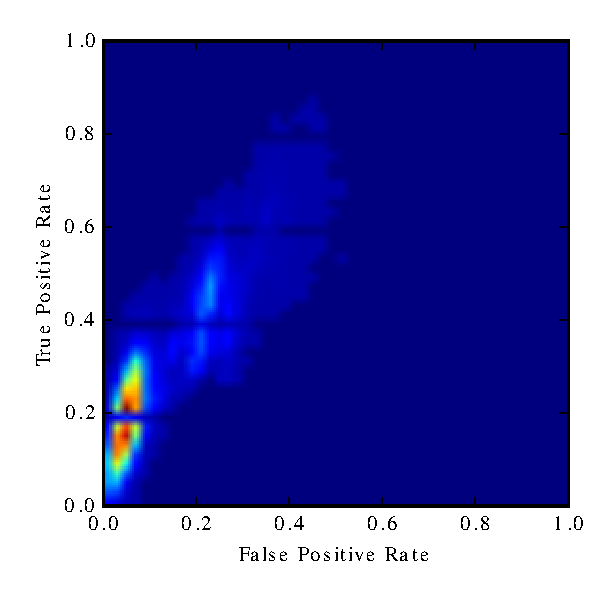
\includegraphics[scale=.9]{recomb15mis/soap.eps}
                	\caption{ROC plot illustrating the density of optical map alignment based missassembly detection classification rates for the SOAPdenovo assembly of {\em Francisella tularensis}. The color intensity at each point indicates the number of three enzyme based classifiers having that classification rate. The plot includes results for optical maps with all three enzyme combinations using a set of 135 enzymes randomly drawn from the REBASE database.  The velvet assembly (which is not shown) has a similar pattern.  Hot spots represent the likely classification rate for enzymes choosen at random.}
                	\label{fig:soap_roc}
        \end{figure}

        \begin{figure}[h!]
            \centering
              	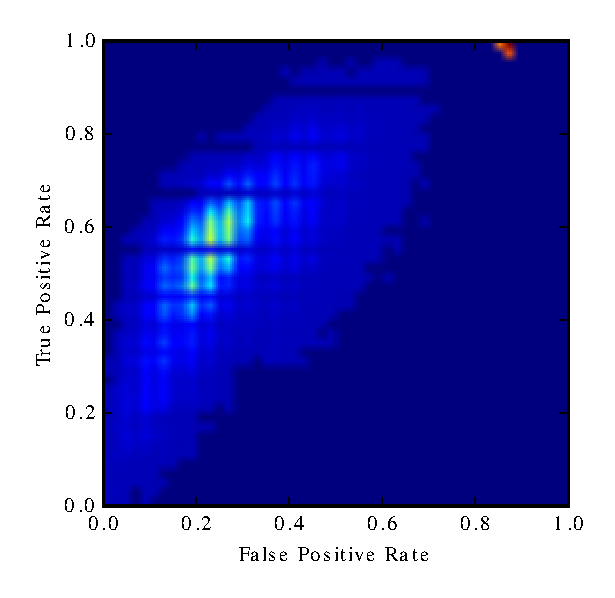
\includegraphics[scale=.9]{recomb15mis/idba.eps}
                	\caption{ROC plot illustrating the density of optical map alignment based missassembly detection classification rates for the IDBA assembly of {\em Francisella tularensis}. The color intensity at each point indicates the number of three enzyme based classifiers having that classification rate. The plot includes results for optical maps with all three enzyme combinations using a set of 135 enzymes randomly drawn from the REBASE database.  Both SPAdes assemblies as well as ABySS (which are not shown) have a similar pattern. Hot spots represent the likely classification rate for enzymes choosen at random.}
                	\label{fig:idba_roc}
        \end{figure}
 

\chapter{Kohdista: A Succinct Solution to Raw Optical Map Alignment}

\makeatletter{}


There is a current resurgence in generating diverse types of data, to be used alone or in concert with short read data, in order to overcome the limitations of short read data.  Data from an optical mapping system~\cite{ORMenc,microfluidic} is one such example and has itself become more practical with high-throughput methods.  For example, the current BioNano Genomics Irys System requires one week and \$1,000 USD to produce the Rmap data for an average size eukaryote genome, whereas, it required \$100,000 and six months in 2009\footnote{http://www.bionanogenomics.com/press-releases/bionano-genomics-launches-irys-a-novel-platform-for-complex-human-genome-analysis/}. These technological advances and the demonstrated utility of optical mapping in genome assembly~\cite{reslewic,zhou,zhou2,amborella,GOAT} have driven several recent tool development efforts~\cite{optima,omblast,maligner}.

Genome-wide optical maps are ordered high-resolution restriction maps that give the position of occurrence of the restriction cut sites corresponding to one or more restriction enzymes.  These genome-wide optical maps are assembled using an overlap-layout-consensus approach using  raw optical map data, which are referred to as {\em Rmaps}.  Hence, Rmaps are akin to reads in genome sequencing.  
{\em To date, however, there is no efficient, non-proprietary method for finding pairwise alignments between Rmaps, which is the first step in assembling genome-wide maps.} 

Several existing methods are superficially applicable to Rmap pairwise alignment, however, all programs either struggle to scale to even moderate size genomes or require significant further adaptation to the problem. One of these is the  dynamic programming method of Valouev {\it et al.}~\cite{Valouev06}, which is capable of solving the problem exactly but requires over 100,000 CPU hours to compute the alignments for rice~\cite{valouev2006algorithm}.   Other methods efficiently find initial seed matches and then extend them through more intensive work.  These include OMBlast~\cite{omblast}, OPTIMA~\cite{optima}, and MalignerIX~\cite{maligner}.  They solve a related alignment problem but are unable to accurately find  pairwise alignments.  This is unsurprising since these methods expect either assembled optical maps or \emph{in silico} digested sequence data for one of their inputs, both having a lower error rate than raw Rmaps.  For example, both OMBlast and OPTIMA found only self alignments on simulated {\em E.coli} (see Results).  MalignerDP is an efficient and error tolerant dynamic programming based method.  However, pairwise alignment for assembly requires overlap alignments and except for Valouev {\it et al.}'s tool, all these tools natively find fit alignments and thus are not readily applicable for these purposes.  OPTIMA prescribes an overlap protocol, but requires the user to break up each Rmap into $k$-mers ($k$-length subsequences) and then align this modified data\footnote{See the $\dopp$ website for a script for this. We provide one since one was unavailable on the OPTIMA website.}. Twin~\cite{wabi2014}, also solves a related problem of aligning {\em in silico } digested contigs to an optical map. 
    










In this paper, we present a fast, error-tolerant method for performing pairwise Rmap alignment that makes use of a novel FM-index-based data structure. The FM-index~\cite{fm2005} itself is key for efficient short read alignment~\cite{BWA,bowtie}, but is difficult to apply directly to Rmap alignment.  This is because of: (1) the Ramp error profile, (2) the fragment sizes require inexact fragment-fragment matches (e.g. 1,547 bp and 1,503 bp represent the same fragment), (3) the Rmap sequence alphabet consists of all unique fragment sizes and is so extremely large (e.g., over 16,000 symbols for the goat genome).  The second two challenges render inefficient the standard FM-index backward search algorithm, which excels at exact matching over small alphabets. The first (and most-notable) challenge requires a more complex index-based data structure be used to create an aligner that is robust for insertion and deletion of cut sites. To overcome these problems, we develop $\dopp$, an index-based Rmap alignment program that is capable of finding all pairwise alignments in large eukaryote organisms.




\paragraph{\protect{\emph{Our contributions.}}}
We first abstract the problem to that of approximate-path matching in a directed 
acyclic graph (DAG). The $\dopp$ method then indexes a set of Rmaps represented
as a DAG, using a modified form of the {\em generalized compressed suffix array (GCSA)}, which is 
a variant of the FM-index developed by Siren et al.~\cite{dag_method}.  The principle insight of our work is that while GCSA is able to efficiently match all similar paths concurrently, it was designed for indexing variations observed in a collection of sequences; all other variations found in a query sequence are handled in query processing. In contrast, our work introduces speculative variations based on the Rmap error profile into the indexed data.  Lastly, we demonstrate that challenges posed by the inexact fragment sizes and alphabet size can be overcome in the GCSA via careful use of a wavelet tree~\cite{GNPtcs11}. 
We verify our approach on simulated {\em E. coli} Rmap data\footnote{The Rmap data is available with the download of our method.} by showing that $\dopp$ achieves similar sensitivity and specificity to Valouev et al., and with more permissive alignment acceptance criteria 90\% of Rmaps pairs with known overlapping genomic origin.  Lastly, we show the utility of our approach on larger eukaryote genomes by demonstrating that existing methods require more than 40 days of CPU time to find all pairwise alignments in the plum Rmap data; whereas, $\dopp$ requires less than two days. 














 
\makeatletter{}\section{Background}
\label{sec-background}


\paragraph{Basic Definitions.}
Throughout we consider a string (or sequence) $S = S[1..n] = S[1]S[2]\ldots$ $S[n]$ of $|S| = n$ 
symbols drawn from the alphabet $[0..\sigma-1]$.
For $i=1,\ldots,n$ we
write $S[i..n]$ to denote the {\em suffix} of $S$ of length $n-i+1$,
that is $S[i..n] = S[i]S[i+1]\ldots S[n]$, and  
$S[1..i]$ to denote the {\em prefix} of $S$ of length $i$.
$S[i..j]$ is the {\em substring} $S[i]S[i+1]\ldots S[j]$ of $S$
that starts at position $i$ and ends at $j$. 
Given a sequence $S[1,n]$ over an alphabet $\Sigma =
\{1,\ldots,\sigma\}$, a character $c \in \Sigma $, and integers
$i$,$j$, $\rank_c(S,i)$ is the number of times that $c$ appears in
$S[1,i]$, and $\select_c(S,j)$ is the position of the $j$-th
occurrence of $c$ in $S$.








\subsubsection{Overview of Optical Mapping.} \label{data_description}

From a computer science viewpoint, restriction mapping (by optical or other means) can be seen as a process that takes in two
sequences: a genome $\A[1,n]$ and a restriction enzyme's recognition sequence $\B[1,b]$, and produces an array (sequence) of integers 
$\C$, the {\em genome restriction map}, which we define as follows. First define the array of integers $\C[1,m]$ where $\C[i] = j$ if and only if 
$\A[j..j+b] = \B$ is the $i$th occurrence of $\B$ in $\A$.
Then $\R[i] = (\C[i]-\C[i-1])$, with $\R[1] = \C[1]-1$.
In words, $\R$ contains the distance between occurrences of $\B$ in $\A$.
For example, if we let $\B = \mbox{{\em act}}$ and 

\begin{center}
  {\setlength{\tabcolsep}{4.5pt}
  {\footnotesize
	\begin{tabular}{p{0.3cm}*{22}{p{0.03cm}}}
		& $\scriptstyle 1 $& $\scriptstyle 2 $& $\scriptstyle 3$& $\scriptstyle 4 $& $\scriptstyle 5 $& 
		$\scriptstyle 6 $& $\scriptstyle 7 $& $\scriptstyle 8 $& $\scriptstyle 9 $& $\scriptstyle 10$&
		$\scriptstyle 11 $& $\scriptstyle 12 $& $\scriptstyle 13$& $\scriptstyle 14 $& $\scriptstyle 15 $& 
		$\scriptstyle 16 $& $\scriptstyle 17 $& $\scriptstyle 18 $& $\scriptstyle 19 $& $\scriptstyle 20$&
		$\scriptstyle 21 $& $\scriptstyle 22 $\\
		$\A = $& $a$ & $t$ & $a$ & $c$ & $t$ & $t$ & $a$ & $c$ & $t$ & $g$ & $g$ 
		&      $a$ & $c$ & $t$ & $a$ & $c$ & $t$ & $a$ & $a$ & $a$ & $c$ & $t$ \\
	\end{tabular}
  }
  }
\end{center}

\noindent then we would have $\C = 3,7,12,15,20$ and $\R = 2,4,5,3,5$.  

In reality, $\R$ is a consensus sequence formed from millions of erroneous Rmap sequences.
The optical mapping system produces millions of Rmaps for a single genome. It is performed on many cells of the organism and for each cell there are thousands of Rmaps (each at least 250 Kbp in length in publicly available data).
The Rmaps are then assembled to produce a genome-wide optical map.
Like the final $\R$ sequence, each Rmap is an array of lengths --- or fragment sizes --- between occurrences of $\B$ in $\A$.

There are three types of errors that an Rmap (and hence with lower magnitude and frequency, also the consensus map) can contain: (1) missing and false cuts, which are caused by an enzyme not cleaving at a specific site, or by random breaks in the DNA molecule, respectively; (2) missing fragments that are caused by {\em desorption}, where small ($ < 1$ Kbp ) fragments are lost and so not detected by the imaging system; and (3) inaccuracy in the fragment size due to varying fluorescent dye adhesion to the DNA and other limitations of the imaging process.  Continuing again with the example above where $\R = 2,4,5,3,5$ is the error-free Rmap: an example of an Rmap with the first type of error could be $\R' = 6,5,3,5$ (the first cut site is missing so the fragment sizes 2, and 4 are summed to become 6 in $\R'$); an example of a Rmap with the second type of error would be $\R'' = 2,4,3,5$ (the third fragment is missing); and lastly, the third type of error could be illustrated by $\R''' = 2,4,7,3,5$ (the size of the third fragment is inaccurately given).  
\paragraph{Frequency of Errors.} In the optical mapping system, there is a 20\% probability that a fragment is missed and a 0.15\% probability of a false break per Kbp, i.e., error type (1) occurs in a fragment.  Popular restiction enzymes in optical mapping experiments recognize a 6 bp sequence giving an expected cutting density of 1 per 4096 bp.  At this cutting density, false breaks are less common than missing restriction sites (approx. $0.25 * .2 = .05$ for missing sites vs. 0.0015 for false sites per bp).  The inaccuracy of the fragment sizes, i.e, error type (3), follows a normal distribution with mean and variance assumed to be 0 bp and $\ell \sigma^2$ ($\sigma = .58$ kbp), respectively~\cite{Valouev06}. 
 
\paragraph{Suffix Arrays, BWT and Backward Search.}
The suffix array~\cite{mm1993} $\SA_{\X}$ (we drop subscripts when
they are clear
from the context) of a sequence $\X$
is an array $\SA[1..n]$ which
contains a permutation of the integers $[1..n]$ such that $\X[\SA[1]..n]
< \X[\SA[2]..n] < \cdots < \X[\SA[n]..n]$.  In other words, $\SA[j] =
i$ iff $\X[i..n]$ is the $j^{\mbox{{\scriptsize th}}}$ suffix of $\X$
in lexicographic order. For a sequence $\Y$, the $\Y$-interval in the suffix array $\SA_{\X}$ is
the interval $\SA[s..e]$ that contains all suffixes having $\Y$ as a
prefix. The $\Y$-interval is a representation of the occurrences of
$\Y$ in $\X$. For a character $c$ and a sequence $\Y$, the computation
of $c\Y$-interval from $\Y$-interval is called a \emph{left extension}.

The Burrows-Wheeler Transform $\BWT[1..n]$ is a
permutation of $\X$ such that $\BWT[i] = \X[\SA[i]-1]$ if $\SA[i]>1$
and $\$$ otherwise \cite{bw1994}. We also define $\LF[i] = j$ iff $\SA[j] =
\SA[i]-1$, except when $\SA[i] = 1$, in which case $\LF[i] = I$,
where $\SA[I] = n$.  Ferragina and Manzini~\cite{fm2005} linked $\BWT$ and $\SA$ in the
following way.  
Let $\C[c]$, for symbol $c$, be the number of symbols
in $\X$ lexicographically smaller than $c$.  The function
$\rank(\X,c,i)$, for sequence $\X$, symbol $c$, and integer $i$, returns
the number of occurrences of $c$ in $\X[1..i]$.  It is well known that
$\LF[i] = \C[\BWT[i]] + \rank(\BWT,\BWT[i],i)$.  Furthermore, we can
compute the left extension using $\C$ and $\rank$.  If $\SA[s..e]$ is
the $\Y$-interval,
then
$\SA[\C[c]+\rank(\BWT,c,s),\C[c]+\rank(\BWT,c,e)]$ is
the $c\Y$-interval.
This is called \emph{backward search}~\cite{fm2005}, and a data
structure supporting it is called an {\em FM-index}.

To support rank queries in backward search, a data structure called a {\em wavelet tree} (see~\cite{GNPtcs11}) 
can be used. It occupies $n\log\sigma + o(n\log\sigma)$
bits of space and supports $\rank$ queries in $O(\log\sigma)$ time.
Wavelet trees also support a variety of more complex queries on the underlying string  efficiently (see, e.g.~\cite{GNPtcs11}). 
One such query we will use in this paper 
is to return the set $X$ of 
distinct symbols occurring in $S[i,j]$, which takes
$O(|X|\log\sigma)$ time.

 
\makeatletter{}\section{The Pairwise Rmap Alignment Problem}



Given a genome $\A[1,n]$ and a restriction enzyme's site $\B[1,b]$, the optical mapping produces Rmaps, which are arrays of lengths---or fragment sizes---between occurrences of $\B$ in $\A$. The background section provides details on the optical mapping process.  Producing Rmap data is an error prone process. Thus, there are three types of errors can occur: (1) missing and false cuts that delimit fragments; (2) missing fragments; and (3) inaccuracy in the fragment sizes.  For example, let $\R = 2,4,5,3,5$ be an error-free Rmap, then an example of an Rmap with the first type of error could be $\R' = 6,5,3,5$ (the first cut site is missing so the fragment sizes 2, and 4 are summed to become 6 in $\R'$); an example of a Rmap with the second type of error would be $\R'' = 2,4,3,5$ (the third fragment is missing); and lastly, the third type of error could be illustrated by $\R''' = 2,4,7,3,5$ (the size of the third fragment is inaccurately given)\footnote{See appendix for a description of the frequency to which these errors occur.}.


The pairwise Rmap alignment problem aims to align one Rmap (the \emph{query}) $\R_q$ against the set of all other Rmaps in the dataset (the \emph{target}). We denote the target database as $\R_1 \ldots \R_n$, where each $\R_i$  is a sequence of fragment sizes, i.e, $\R_i = [f_{i1}, .., f_{im_i}]$.  An alignment between two Rmaps is a relation between them comprising groups of zero or more consecutive fragment sizes in one Rmap to groups of zero or more consecutive fragments in the other.  For example, given $\R_i =  [4, 5, 10, 9, 3]$ and $\R_j = [10, 9, 11]$ one possible alignment is $\{[4,5], [10]\}, \{ [10], [9]\}, \{[9], [11]\}, \{[3], []\}$.  A group may contain more than one fragment (e.g. $[4,5]$) when the restriction site delimiting the fragments is absent in the corresponding group of the other Rmap (e.g $[10]$). This can occur if there is a false restriction site in one Rmap, or there is a missing restriction site in the other.  Since we cannot tell from only two Rmaps which of these scenarios occurred, for the purpose of our remaining discussion it will be sufficient to consider only the scenario of missed (undigested) restriction sites. 

 
\makeatletter{}
\section{Methods}\label{sec-meods}

We now describe the algorithm behind $\dopp$.
Three main insights enable our index-based aligner for Rmap data: 1) abstraction of the alignment problem to a finite automaton; 2) use of the GCSA for storing and querying the automaton; and 3) modification of backward search to use a wavelet tree in specific ways to account for the Rmap error profile.  
\subsection{Finite Automaton.}

Continuing with the example in the background section, we want to align $\R' = 6,5,3,5$ to $\R''' = 2,4,7,3,5$ and vice versa.  To accomplish this we cast the Rmap alignment problem to that of matching paths in a finite automaton.  A finite automaton is  a directed, labeled graph that defines a \emph{language}, or a specific set of sequences composed of vertex labels.  A sequence is recognized by an automaton if it contains a matching path: a consecutive sequence of vertex labels equal to the sequence. We represent the target Rmaps as an automaton and the query as a path in this context.  

The automaton for our target Rmaps can be constructed as follows.  First concatenate the $\R_1 \ldots \R_n$ together into a single sequence with each Rmap separated by  a special symbol which will not match any query symbol. Let $\R^*$ denote this concatenated sequence. Hence, $\R^* = [f_{11},..,f_{1m_1}, \ldots, f_{n1},..,f_{nm_n}]$.  Then, construct an initial finite automaton $\A = (V, E)$ for $\R^*$ by creating a set of vertices $v^i_1 .. v^i_m$, one vertex labeled with each fragment length and edges connecting them.Also, introduce to $\A$  a {\em starting vertex} $v_1$ labeled with $\#$ and a {\em final vertex} $v_f$ labeled with the character $\$$.  All other vertices in $\A$ are labeled with integral values.  This initial set of vertices and edges is called the {\em backbone}.  The backbone by itself is only sufficient for finding alignments with no missing cut sites in the query. Figure \ref{fig:example}(a) illustrates the construction of $\A$ for a single Rmap.  The backbone of this automaton is $\#, 2, 3, 4, 5, 6, \$$.  Next, extra vertices (``skip vertices'') and extra edges are added to $\A$ to allow for the automaton to accept all valid queries.  

\paragraph{Skip Vertices and Skip Edges.}
We introduce additional vertices labeled with {\em compound fragments} to allow missing cut sites (first type of error) to be taken into account in querying the target Rmaps.  We refer to these as {\em skip vertices} as they provide alternative path segments which skip past two or more backbone vertices. Thus, we add a {\em skip vertex} to $\A$ for every $o+1$ length run of consecutive vertices in the backbone where $1 < o < order$ and  \emph{order} is the maximum number of consecutive missed cut sites to be accommodated.  First order skip vertices are each labeled with the sum of two consecutive backbone vertices.  Second order skip vertices are each labeled with the sum of three consecutive backbone vertices. The vertex labeled with $7$ connecting $2$ and $5$ in \ref{fig:example}(a) is an example of a skip vertex.  Likewise, $5, 9, 11$ are other skip vertices.




Finally, we add {\em skip edges} which provide paths around vertices with small labels in the backbone.
These allow a query with a missing fragment to still match.\footnote{Different smallness thresholds for query and target bias toward this scenario, avoiding backtracking in the search.}  Hence, the addition of skip edges allow for desorption (the second type of error) to be taken into account in querying the target Rmaps.  



\subsection{The Rmap Alignment Score.}

Alignments are found by incrementally extending candidate partial alignments (paths in the automaton) to longer partial alignments by choosing one of several compatible extension matches (adjacent vertices to the end of a path in the automaton).  To perform this search efficiently, we prune the search by a scoring model that scores the size agreement of the matched compound fragments, and the frequency of putative missing cut sites.

\paragraph{Size Agreement.}
We use the Chi-square CDF statistic to assess size agreement.  This assumes the fragment size errors are independent, normally distributed events.  For each pair of matched compound fragments in a partial alignment, we take the average between the two as the assumed true length and
compute the expected standard deviation using this mean.  Each compound fragment deviates from the assumed true value by half the distance between them.  These two deviation values contribute two degrees of freedom to the Chi-square calculation.

\paragraph{Cut Site Error Frequency.}
We use the Binomial CDF statistic to assess the probability of the number of cut site errors in a partial alignment.   This assumes missing cut site errors are independent, Bernoulli processes events.  We account for all the putatively conserved cut sites on the boundaries and those delimiting compound fragments in both partially aligned Rmaps plus twice the number of missed sites as Bernoulli trials. 
Thus, given a set of Rmaps and input parameters $\rho_{L}$ and $\rho_{U}$, we produce the set of all Rmap alignments that have a chi-square CDF statistic less than $\rho_U$ and a binomial CDF statistic less than $\rho_L$.  Both of these are subject to the additional constraint of a maximum consecutive missed restriction site run between aligned sites of $\delta$ and a minimum aligned site set cardinality of 16. 

 
\makeatletter{}
\begin{figure*}[h!]
 \centering
 \includegraphics[width=0.6\textwidth]{../content/figures/example_combined}
  \caption{(a) shows an example automaton.  The top half of vertices contains the label, which models a fragment size in Kbp.  The common prefixes of all suffixes spelled from a vertex is written in the bottom half.  Note that there is no ordering of vertices such that all their corresponding suffixes are in lexicographic order;  the leftmost vertex labelled with ``5'' spells suffixes beginning ``5,4,...'' as well as the suffix ``5,9,6,\$'' while the rightmost $5$  spells the suffix ``5,6,\$''. (b) shows the prefix sorted automaton corresponding to the one in (a).  The leftmost vertex $5$ has been duplicated and the outgoing edges of the previous version have been divided between the new replacement instances.  This also divides the suffixes spellable from the prior version.  Now the three $5$ vertices can be ordered based on their common prefixes as [``$5$,$4$,...'',``$5$,$6$,\$'', ``$5$,$9$,$6$, \$'']. }
\label{fig:example}
\end{figure*}

\begin{table*}[h!]
\begin{center}
  \begin{tabular}{ccccccccccccc}
  	\hline
		& \$		& 2		& 3		& 4		& 5,4		& 5,6,\$	& 5,9,6,\$	& 6,\$	& 7	& 9,6,\$	& 11,\$	& \# \\
	\hline
$\BWT$	& 6,11	& \#		& 2		& 3,5		& \#		& 4,7		& \#		& 5,9		& 2	& 3,5		& 4,7		& \$ \\
$\M$		& 1		& 10		& 10		& 10		& 1		& 1		& 1		& 1		&10	& 1		& 1 		& 100 \\
$\F$		& 10		& 1		& 1		& 10		& 1		& 10		& 1		& 10		& 1	& 10		& 10		& 1 \\		
	\hline
	\end{tabular}
      \caption{Table listing the three arrays storing the automaton in memory: $\BWT$, $\M$, and $\F$.}
 \label{bwt-table}
\end{center}
\end{table*}


\subsection{Generalized Compressed Suffix Array.}


We index the automaton with the GCSA~\cite{dag_method} for efficient storage and path querying.  The GCSA is a generalization of the FM-index for automata and
we will explain the GCSA by drawing on the definition of the (more widely known) FM-index.  As stated in the background section, the FM-index is based on the deep relationship between the $\SA$ and the $\BWT$ data structures of the input string $\X$. The $\BWT$ of an input string is formed by sorting all characters of the string by the lexicographic order of the suffix immediately following each character.  The main properties the FM-index exploits in order to perform queries efficiently are a) $\BWT[i] = \X[\SA[i]-1]$; and 
b) given that $\SA[i] = j$, and $\C[c]$ gives the position of the first suffix in $\SA$ prefixed with character $c$, then using small auxiliary data structures we can quickly determine $k = \C[\BWT[i]] + \rank(\BWT,\BWT[i],i)$, such that $\SA[k] = j-1$.
The first of these properties is simply the definition of the $\BWT$.  The second is, because the symbols of $\X$ occur in the same order in both the single character prefixes in the suffix array and in the $\BWT$, given a set of sorted suffixes, prepending the same character onto each suffix does not change their order. Thus, if we consider all the suffixes in a range of $\SA$ which are preceded by the same symbol $c$, that subset will appear in the same relative order in (another part of) $\SA$: as a contiguous subinterval of the interval that contains all the suffixes beginning with $c$. Thus by knowing where a symbol's run begins in the $\SA$ and the $\rank$ of an instance of that symbol, we can identify the $\SA$ position beginning with that instance from its position in $\BWT$. A rank data structure over the $\BWT$ thus constitutes a compressed version of the suffix array. 





To generalize the FM-index to automata (from strings), we need to efficiently store the vertices and edges in a manner such that the FM-index properties still hold, allowing the GCSA to support queries efficiently.  An FM-index's compressed suffix array for a string $S$ encodes a relationship between each suffix $S$ and its left extension.  Hence, this suffix array can be generalized to edges in a graph that represent a relationship between vertices.  The compressed suffix array for a string is a special case where the vertices are labeled with the string's symbols in a non-branching path. 
\paragraph{Prefix-sorted automata.}
Just as backward search for strings is linked to suffix sorting, backward searching in the BWT of the automaton 
requires us to be able to sort the vertices (and a special set of the paths) of the automaton in a particular 
way. In~\cite{dag_method} this property is called {\em prefix-sortedness}. Let $A = (V,E)$ be a finite automaton, 
let $v_{|V|}$ denote its terminal vertex, and let $v \in V$ be a vertex. We say $v$ is {\em prefix-sorted} by 
prefix $p(v)$ if the labels of all paths from $v$ to $v_{|V|}$ share a common prefix $p(v)$, and no path from any 
other vertex $u \ne v$ to $v_{|V|}$ has $p(v)$ as a prefix of its label. Automaton $A$ is prefix-sorted if all 
vertices are prefix-sorted. See Figure~\ref{fig:example} for an example of a non-prefix sorted automaton and a 
prefix sorted automaton. A non-prefix sorted automaton can be made prefix sorted through a process of duplicating 
vertices and their incoming edges but dividing their outgoing edges between the new instances (see~\cite{dag_method}).

Clearly the prefixes $p(v)$ allow us to sort the vertices of a prefix-sorted automaton into lexicographical 
order. Moreover, if we consider the list of outgoing edges $(u,v)$, sorted by pairs $(p(u),p(v))$, they are
also sorted by the sequences $\ell(u)p(v)$, where $\ell(u)$ denotes the label of vertex $u$. This (dual sortedness)
property allows backward searching to work over the list of vertex labels (sorted by $p(v)$) in the same way
that is does for the symbols of a string ordered by their following suffixes in normal backward search for 
strings.

Each vertex has a set of one or more preceding vertices and therefore, a set of predecessor labels in the 
automaton. These predecessor label sets are concatenated to form the $\BWT$. The sets are concatenated the 
order defined by the above mentioned lexicographic ordering of the vertices. Each element in $\BWT$ then 
denotes an edge in the automaton. Another array of bits, $\F$, marks a `1' for the first element of $\BWT$ 
corresponding to a vertex and a `0' for all subsequent elements in that set. Thus, the predecessor labels, 
and hence the associated edges, for a vertex with rank $r$ are $\BWT[\select(r)..\select(r+1)]$. Another 
array, $\M$, stores the out degree of each vertex and allows the set of vertex ranks associated with a $\BWT$ 
interval to be found using $\rank()$ queries.



 







 


\subsection{Exact Matching: GCSA Backward Search.}


Exact matching with the GCSA is similar to the standard FM-index backward search algorithm. As outlined in the background section, FM-index backward search proceeds by finding a succession of lexicographic ranges that progressively match longer and longer suffixes of the query string, starting from the rightmost symbol of the query. The search maintains two items --- a lexicographic range and an index into the query string --- and the property that the path prefix associated with the lexicographic range is equal to the suffix of the query marked by the query index. Initially, the query index is at the rightmost symbol and the range is $[1..n]$ since every path prefix matches the empty suffix.  The search continues using GCSA's backward search step function, which takes as parameters the next symbol (to the left) in the query (i.e. fragment size in $\R_q$) and the current range, and returns a new range.  The query index is advanced leftward after each backward search step.  In theory, since the current range corresponds to a consecutive range in the $\BWT$, the backward search could use use $\select()$ queries on a bit vector $\F$ to determine all the edges adjacent to a given vertex and then two FM-index $\LF()$ queries are applied to the limits of the current range to obtain the new one.  GCSA's implementation uses one succinct bit vector per alphabet symbol to encode which symbols precede a given vertex instead of $\F$.  Finally, this new range, which corresponds to a set of edges, is mapped back to a set of vertices using $\rank()$ on the $\M$ bit vector.







\subsection{Inexact Matching: GCSA Backward Search Using a Wavelet Tree.}




We modified backward search in the following ways:
(1) we used a wavelet tree to allow efficient retrieval of substitution candidates; (2) we modified the search process to combine consecutive query fragments into compound fragments so as to match fragments in $\R^*$ missing the interposing restriction site; and (3) we introduced backtracking, in order to try substitution candidates and combinations of compound fragment. These modifications are further detailed below.

First, in order to accommodate possible errors in fragment size, we determine a set, $\D$, of candidate fragment sizes that are similar to the next fragment of $\R_q$ to be matched in the query. These candidates are determined by enumerating the distinct symbols in the currently active backward-search range of the $\BWT$ using the wavelet tree algorithm of Gagie et al.~\cite{GNPtcs11}.  This requires introducing bit array $\F$ into the actual implementation\footnote{Recall that this active range, when applied to a lexicographic range, represents the suffixes whose prefixes are the matched portion of the query, while the same range of the $\BWT$ contains possible extension symbols.}. To accommodate possible restriction sites that are present in the query Rmap but absent in target Rmaps, we generate compound fragments (i.e. new symbols) by summing pairs and triples of consecutive query fragment size and then querying the wavelet tree for substitutions of these compound fragments. This summing of multiple consecutive fragments is complementary to the skip vertices in the target automaton and accommodates missed restriction sites in the target, just as the skip vertices accommodate missed sites in the query.  





 

Lastly, since there may be multiple match candidates in the $\BWT$ interval of $\R^*$ 
for a compound fragment drawn from $\R_q$, we add backtracking to backward search so that each candidate size returned to the search algorithm from the wavelet tree is evaluated; i.e., for a given compound fragment size $f$ generated from $\R_q$, every possible candidate fragment size, $f'$, that can be found in $\R^*$ in the range $f - t \ldots f + t$ and in the interval $s \ldots e$ (of the $\BWT$ of $\R^*$) for some tolerance $t$ is used as a substitute in the backward search. Each of these candidates is then checked to ensure that the longer partial alignment formed by a left extension would still satisfy alignment criteria.  This requires the alignment criteria be \emph{monotone}, that is, that the prefixes of a credible long alignment are also credible alignments.  Since the chi-square and binomial CDF statistics are p-values, they make suitable alignment criteria.   When this criteria is still satisfied after including a candidate symbol, it is used as the extension symbol in the backward search.
 
 





 
\makeatletter{}\label{sec-results}


We evaluated $\dopp$ against the other available nonproprietary optical map alignment software.
Our experiments measured runtime, peak memory, and  alignment count on simulated {\em E. coli} Rmaps and experimentally generated plum Rmaps.  All experiments were performed on Intel Xeon workstations with $\ge$ 16 GB RAM running 64-bit Linux.

$\dopp$ was configured to run using 100 bp bins for quantization, a minimum match length parameter of 15 compound fragments, a $\chi^2$ CDF threshold of 0.05, a binomial CDF threshold of 0.45 and two orders of skip nodes.
The software of Valouev et al., the only package designed for pairwise Rmap alignment, was run with default parameters except we reduced the maximum compound fragment length (their $\delta$ parameter) from 6 fragments to 3. We observed the software of Valouev et al. rarely included alignments containing more than two missed restriction sites in a compound fragment, hence we compare all tools, where adjustable, with this compound fragment size limit.

Other tools were designed for less noisy data, but in theory could address all the data error types required. We adjusted parameters for pairwise Rmap alignment where possible and test them as well. We tried OPTIMA with both ``p-value'' and ``score'' scoring and the allMaps option and report the higher sensitivity ``score'' setting.  We followed the OPTIMA-Overlap protocol of splitting Rmaps into $k$-mers, each containing 12 fragments as suggested in~\cite{optima}.
OMBlast~\cite{omblast} was run with its default settings.
MalignerDP was run with the options ``--ref-max-misses 2 --query-miss-penalty 3.0 --query-max-miss-rate 0.50''.



Gentig~\cite{Anantharaman01} and BACop~\cite{Zhou09} were not available for download so could not be tested. SOMA~\cite{Nagarajan08} could potentially align Rmap data, but implements a dynamic programming algorithm similar in spirit to that of Valouev et al. and allows an unbounded number of consecutive missed sites and is thus computationally even more expensive (see~\cite{wabi2014}).  MalignerIX indexes nodes in a DAG akin to ours and uses them as initial seed matches before reverting to exhaustive search.  However, it only allows missing site errors in the target Rmaps.  $\twin$~\cite{wabi2014} assumes consensus optical map inputs (with no missing restriction sites), so was not included.





\subsection{Performance on Simulated E.coli Rmap Data.} \label{sec:ecoli}

To verify the correctness of our method, we simulated a read set from the 4.6 Mbp \emph{E. coli} reference genome as follows:  we started with 1,400 copies of the genome, and then generated 40 random loci within each. These loci form the ends of molecules that would undergo digestion.  Molecules smaller than 250 Kbp were discarded leaving 272 molecules with a combined length equating to 35x coverage depth.  The cleavage sites for the XhoI enzyme were then identified within each of these simulated molecules. We removed 20\% of these at random from each simulated molecule to model partial digestion.  Finally, normally distributed noise was added to each fragment with a standard deviation of .58 kb per 1 kb of the fragment.  Simulated molecule pairs having 16 common conserved digestion sites become the ``ground truth''\footnote{Due to repeats in the restriction map, and apparent repeats at the resolution attainable through optical measurement, some alignments beyond these are expected.} data for testing our method with the others.  This method of simulation was based on the \emph{E. coli} statistics given by Valouev et al.~\cite{valouev2006algorithm} and resulting in a molecule length distribution as observed in publicly available Rmap data from OpGen, Inc.
Our  alignment results on simulated data are summarized in Table~\ref{tbl-ecoli}.  

OPTIMA and OMBlast were only able to find alignments between a given Rmap and itself were so not tested further on plum.  

$\dopp$ uses $\chi^2$ and binomial CDF thresholds to prune the backtracking search when deciding whether to extend alignments to progressively longer alignments.  More permissive match criteria, using higher thresholds, allows  more Rmaps to be reached in the search and thus considered aligned, but it also results in less aggressive pruning in the search, thus lengthening runtime.  When $\dopp$ was configured with a CDF threshold of .5 and a binomial CDF threshold of .7, it found 4,100 of the 4,305 (91\%) ground truth alignments. 






\begin{table*}[htb]
  \small
  \centering
  \begin{tabular}{l|l|l|l|l}
	{\bf Method}	& {\bf Time}		& {\bf Memory} 	& {\bf Alignments } & {\bf Fraction of Ground Truth}\\
	\hline
	\hline
	   	 $\dopp$ ($\chi^2$  $<$ .02, Binom. $<$ .5)    	 	& 20 s.		& 19.0 MB & 907 & 702 / 4,305  (16\%)\\
   	 $\dopp$ ($\chi^2$  $<$ .5, Binom. $<$ .6)    	 	& 373 s. 		& 18.3 MB & 8,545	& 3,925 / 4,305 (91\%) \\
	Valouev et al. 		& 148 s. 	& 4.0 MB		&  742 & 699 / 4,305 (16\%) \\
    MalignerDP          & 19 s.     & 5.7 MB        & 2,134 & 1,150 / 4,305 (27\%) \\
    OMBlast              & 10 s.     & 45.0 MB       & 272  & 0 / 4,305 (0\%) \\
    OPTIMA              & 455 s.     & 10,756.5 MB       & 272  & 0 / 4,305 (0\%) \\    
	\end{tabular}
      \caption{Performance on simulated {\it E. coli} dataset.}
 \label{tbl-ecoli}
\end{table*}






\subsection{Performance on Plum Rmap Data.} \label{section:plum}

The Beijing Forestry University
and other institutes assembled the first plum ({\em Prunus mume}) genome, of approximately 280 Mbp.  
This assembly is of significant agricultural importance, providing an initial understanding of the evolution of fruit trees~\cite{plum}.  For this species, several diverse datasets were generated, including short read data 
and optical mapping data generated from OpGen Inc. using the BamHI enzyme, 
and is available in the GigaScience repository.
We use data from June, 2011, consisting of 139,281 Rmaps having coverage depth of 135x.

Our results on this plum dataset are summarized in Table~\ref{tbl-plum} and described as follows.  Although MalignerDP can cope with the high error rate, by design it only finds alignments where one Rmap aligns entirely within the bounds of another, while overlap alignments are required for assembling a whole genome map. $\dopp$, configured with a $\chi^2$ CDF threshold of .025, took 124 hours of CPU time to search for alignments across the plum Rmap data, representing an 32x speedup of the 1,001 hours taken by the Valouev et al. software.  The alignment used a peak of 7.4 GB of RAM.  Building the GCSA data structure required 11  minutes and required 13 GB of RAM.

\begin{table}[h!]
  \small
  \centering
  \begin{tabular}{l|l|l|l}
	{\bf Method}	& {\bf Time}		& {\bf Memory} 	& {\bf Alignments } \\
	\hline
	\hline

   	 $\dopp$    	 	& 31 hours		& 7.4 GB  & 16,109,151 \\
	Valouev et al. 		& 1,001 hours 	& 61 MB		&  6,387  \\
    MalignerDP          & 222 hours     & 772 MB    & 1,309,640 \\
	\end{tabular}
      \caption{Performance on Plum.}
 \label{tbl-plum}
\end{table}

We note that our indexing method can find any alignment pattern that a dynamic program method can, with differing results only arising from different scoring functions.  Even with our simplistic one, our results from \emph{E. coli} simulation demonstrate comparable capability in finding alignments to Valouev {\it et al.}'s software.  Additionally, these results show that for these same parameter settings our method yields significant speedup on eukaryote scale Rmap data.  



 

\chapter{Succinct Colored de Bruijn Graphs}
\makeatletter{}




  \section{Motivation:}
  Iqbal et al. (Nature Genetics, 2012) introduced the {\em colored de Bruijn graph}, a variant of the classic de Bruijn graph, which is aimed at ``detecting and genotyping simple and complex genetic variants in an individual or population''.
Because they are intended to be applied to massive population level data, it is essential that the graphs be represented efficiently.
Unfortunately, current succinct de Bruijn graph representations are not directly applicable to the colored de Bruijn graph, which requires additional information to be succinctly encoded as well as support for non-standard traversal operations.
\section{Results:}
Our data structure dramatically reduces the amount of memory required to store and use the colored de Bruijn graph, with some penalty to runtime, allowing it to be applied in much larger and more ambitious sequence projects than was previously possible.
\section{Availability:} https://github.com/cosmo-team/cosmo/tree/VARI
 
\makeatletter{}

In the 20 years since it was introduced to bioinformatics by ~\cite{IW95}, the {\em de Bruijn graph} has become a mainstay of modern genomics, essential to genome assembly~\citep{how,sequel,ismb2015}. The near ubiquity of de Bruijn graphs has led to a number of succinct representations, which aim to implement the graph in small space, while still supporting fast navigation operations.  Formally, a de Bruijn graph constructed for a set of strings (e.g., sequence reads) has a distinct vertex $v$ for every unique $(k - 1)$-mer (substring of length $k - 1$) present in the strings, and a directed edge $(u, v)$ for every observed $k$-mer in the strings with $(k - 1)$-mer prefix $u$ and $(k - 1)$-mer suffix $v$. A contig corresponds to a non-branching path through this graph. See~\citep{how} for a more thorough explanation of de Bruijn graphs and their use in assembly. 

\cite{ICTFM12} introduced the {\em colored de Bruijn graph}, a variant of the classical structure, which is aimed at ``detecting and genotyping simple and complex genetic variants in an individual or population.'' The edge structure of the colored de Bruijn graph is the same as the classic structure, but now to each vertex ($(k - 1)$-mer) and edge ($k$-mer)
is associated a list of colors corresponding to the samples in which the vertex or edge label exists. More specifically, given a set of $n$ samples, there exists a set $\mathcal{C}$ of $n$ colors $c_1, c_2, .., c_n$ where $c_i$ corresponds to sample $i$ and all $k$-mers and $(k-1)$-mers that are contained in sample $i$ are colored with $c_i$. A {\em bubble} in this graph corresponds to an undirected cycle, and is shown to be indicative of biological variation by \cite{ICTFM12}. 
{\sc Cortex}, the implementation of \cite{ICTFM12}, uses the colored de Bruijn graph to develop a method of assembling multiple genomes simultaneously, without losing track of the individuals from which $(k - 1)$-mers (and $k$-mers) originated. This graph is derived from either multiple reference genomes, multiple samples, or a combination of both.

Variant information of an individual or population can be deduced from structure present in the colored de Bruijn graph and the colors of each $k$-mer.
As implied by \cite{ICTFM12}, the ultimate intended use of colored de Bruijn graphs is to apply it to massive, population-level sequence data that is now abundant due to next generation sequencing technology (NGS) and multiplexing. These technologies have enabled production of sequence data for large populations, which has led to ambitious sequencing initiatives that aim to study genetic variation for agriculturally and bio-medically important species.  These initiatives include the {\em Genome 10K} project that aims to sequence the genomes of 10,000 vertebrate species~\citep{Haussler:2009}, the {\em iK5} project~\citep{Robinson:2011}, the 150 Tomato Genome ReSequencing project~\citep{tomato1,tomato2}, and the 1001 Arabidopsis project, a worldwide initiative to sequence cultivars of {\em Arabidopsis}~\citep{arabidopsis}.  Hence, the succinct colored de Bruijn graph is applicable in the context of these projects, in that it can assist in variation discovery within a species by analyzing all the data in these projects at once. 

In addition to species-specific initiatives, scientific and regulatory agencies are showing increased interest in shotgun metagenomic sequences for public health purposes~\citep{EMBL-EBI-Metagenomics,Miller2013}, specifically monitoring for antimicrobial resistance (AMR)~\cite{baquero_metagenomic_epi, port_2014_metagenomics_AMR_monitoring}.  AMR is considered one of the top public health threats, with fears that the spread of AMR will lead to increased morbitiy and mortality for many bacterial illnesses~\citep{CARB,FAOActionPlan2016}.  AMR occurs when bacteria express genetic elements that render them impervious to antibiotic treatments.  Importantly, these genetic resistance elements can be exchanged between distantly-related bacteria via multiple genetic mechanisms, which makes AMR an inherently population-level phenomenon~\citep{Baquero2013}.   Shotgun metagenomic sequencing allows access to the entire microbial population in a sample (the "metagenome"), which is of immense value for tracking and understanding the evolution of resistance elements within and across diverse bacteria\citep{MacLean2010}.  This metagenomics approach to AMR surveillance has been applied in both human and agricultural settings~\citep{noyes2016resistome,King2016}, generating hundreds of samples with terabytes of sequence data for relatively small studies.  Given the large number of samples and large size of sequence data involved in these whole-genome and metagenomic projects, it is imperative that the colored de Bruijn graph can be stored and traversed in a space- and time-efficient manner.
 

\paragraph{Our Contribution}  
We develop an efficient data structure for storage and use of the colored de Bruijn graph. Compared to {\sc Cortex}, the implementation of \cite{ICTFM12}, our new data structure dramatically reduces the amount of memory required to store and use the colored de Bruijn graph, with some penalty to runtime. We demonstrate this reduction in memory through a comprehensive set of experiments across the following three datasets: (1)  four plant genomes, (2) 3,765 {\em Escherichia coli} assemblies,
 and (3) 87 sequenced metagenomic samples from commercial beef production facilities.  We show our method, which we refer to as $\ours$ (Finnish for color), has better peak memory usage on all these datasets. Our plant reference genomes dataset required 101 GB of RAM for  {\sc Cortex} to represent while $\ours$ required only 4 GB.  And  our
largest two datasets contain too many $k$-mers and colors for {\sc Cortex}'s data structure to represent in the 512 GB of RAM available on our bioinformatics servers. $\ours$ is a novel generalization of the succinct data structure for classical de Bruijn graphs due to \cite{BOSS12}, which is based on the Burrows-Wheeler transform of the sequence reads, and thus, has independent theoretical importance.

In addition to demonstrating the memory and runtime of $\ours$, we validate its output using the {\em E.coli} reference genome and a simulated variant.


\paragraph{Related Work} As noted above, maintenance and navigation of the de Bruijn graph is a space and time bottleneck in genome assembly. Space-efficient representations of de Bruijn graphs have thus been heavily researched in recent years. One of the first approaches was introduced by \cite{Simpson:2009} as part of the development of the ABySS assembler.  Their method stores the graph as a distributed hash table and thus requires 336 GB to store the graph corresponding to a set of reads from a human genome (>38x depth paired-end reads from Illumina Genome Analyzer II, HapMap: NA18507\footnote{\url{https://www.ncbi.nlm.nih.gov/sra/?term=SRA010896}}). 
 
 \cite{conway} reduced space requirements by using a sparse bitvector  (by \cite{bitvector}) to represent the $k$-mers (the edges), and used rank and select operations (to be described later) to traverse it. As a result, their representation took 32 GB for the same data set.  Minia, by \cite{wabi}, uses a Bloom filter to store edges. They traverse the graph by generating all possible outgoing edges at each node and testing their membership in the Bloom filter. Using this approach, the graph was reduced to 5.7 GB on the same dataset.  Contemporaneously, \cite{BOSS12} developed a different succinct data structure based on the Burrows-Wheeler transform~\citep{BW94} that requires 2.5 GB.  The data structure of \cite{BOSS12} is combined with ideas from IDBA-UD~\citep{idbaud} in a metagenomics assembler called MEGAHIT~\citep{megahit}.  In practice MEGAHIT requires more memory than competing methods  but produces significantly better assemblies.   \cite{paul} implemented the de Bruijn graph using an FM-index and {\em minimizers}.   Their method uses 1.5 GB on the same NA18507 data.  \cite{BFT} released the Bloom Filter Trie, which is another succinct data structure for the colored de Bruiin graph; however, we were unable to compare our method against it since  it only supports the building and loading of a colored de Bruijn graph and does not contain operations to support our experiments.  SplitMEM~\citep{splitmem} is a related algorithm to create a colored de Bruijn graph from a set of suffix trees representing the other genomes. Lastly, Lin et al. \citep{Lin} point out the similarity between the breakpoint graph, which is traditionally viewed as a data structure to detect breakpoints between genome rearrangements, and the colored de Bruijn graph. 
 

\paragraph{Roadmap} In the next section, we describe our succinct colored de Bruijn graph data structure, generalizing the stucture for classic de Bruijn graphs presented by ~\cite{BOSS12}. Section~\ref{sec:results} then elucidates the practical performance of the new data structure, comparing it to {\sc Cortex}. Section~\ref{sec:conclusion} offers some concluding remarks.

 
\makeatletter{}\label{sec:methods}

Our data structure for colored de Bruijn graphs is based on the succinct representation of individual de Bruijn graphs introduced by \cite{BOSS12}---which we refer to as the BOSS representation from the authors' initials---so we start by describing that representation.  We note that BOSS is itself a generalization of FM-indexes~\citep{FM05} obtained by extending the Burrows-Wheeler transform (BWT) from strings to the multisets of edge-labels of de Bruijn graphs.  We then give a general explanation of how we add colors, and finally give details of our implementation.

\subsection{BOSS Representation}
\label{subsec:boss}

Consider the de Bruijn graph \(G = (V, E)\) for a set of $k$-mers, with each $k$-mer \(a_0 \cdots a_{k - 1}\) representing a directed edge from the node labelled \(a_0 \cdots a_{k - 2}\) to the node labelled \(a_1 \cdots a_{k - 1}\), with the edge itself labelled \(a_{k - 1}\).  Define the nodes' co-lexicographic order to be the lexicographic order of their reversed labels.  Let $F$ be the list of $G$'s edges sorted co-lexicographically by their ending nodes, with ties broken co-lexicographically by their starting nodes (or, equivalently, by their $k$-mers' first characters).  Let $L$ be the list of $G$'s edges sorted co-lexicographically by their starting nodes, with ties broken co-lexicographically by their ending nodes (or, equivalently, by their own labels).  If two edges $e$ and $e'$ have the same label, then they have the same relative order in both lists; otherwise, their relative order in $F$ is the same as their labels' lexicographic order.  Defining the edge-BWT (EBWT) of $G$ to be the sequence of edge labels sorted according to the edges' order in $L$, so \(\elabel (L [h]) = \EBWT (G) [h]\) for all $h$, this means that if $e$ is in position $p$ in $L$, then in $F$ it is in position
\begin{equation*}
|\{d\,:\,d \in E,\ \elabel (d) \prec \elabel (e)\}| + \EBWT (G).\rank_{\elabel (e)} (p) - 1\,,
\end{equation*}
where \(\EBWT (G).\rank_{\elabel (e)} (p)\) is the number of times $\elabel (e)$ appears in \(\EBWT (G) [1,p]\).  It follows that if we have, first, an array storing \(|\{d\,:\,d \in E,\ \elabel (d) \prec c\}|\) for each character $c$ and, second, a fast rank data structure on \(\EBWT (G)\) then, given an edge's position in $L$, we can quickly compute its position in $F$.

Let $B_F$ be the bitvector with a 1 marking the position in $F$ of the last incoming edge of each node, and let $B_L$ be the bitvector with a 1 marking the position in $L$ of the last outgoing edge of each node.  Given a character $c$ and the co-lexicographic rank of a node $v$, we can use $B_L$ to find the interval in $L$ containing $v$'s outgoing edges, then we can search in \(\EBWT (G)\) to find the position of the one $e$ labelled $c$.  We can then find $e$'s position in $F$, as described above.  Finally, we can use $B_F$ to find the co-lexicographic rank of $e$'s ending node.  With the appropriate implementations of the data structures, we can store $G$ in \((1 + o (1)) |E| (\lg \sigma + 2)\) bits, where $\sigma$ is the size of the alphabet (i.e., 4 for DNA), such that when given a character $c$ and the co-lexicographic rank of a node $v$, in $\Oh{\log \log \sigma}$ time we can find the node reached from $v$ by following the directed edge labelled $c$, if such an edge exists.

If we know the range \(L [i..j]\) of $k$-mers whose starting nodes end with a pattern $P$ of length less than \((k - 1)\), then we can compute the range \(F [i'..j']\) of $k$-mers whose ending nodes end with \(P c\), for any character $c$, since
\begin{eqnarray*}
    i' & = & |\{d\,:\,d \in E,\ \elabel (d) \prec c\}| + \EBWT (G).\rank_c (i - 1)\\ 
    j' & = & |\{d\,:\,d \in E,\ \elabel (d) \prec c\}| + \EBWT (G).\rank_c (j) - 1\,.
\end{eqnarray*}
It follows that, given a node $v$'s label, we can find the interval in $L$ containing $v$'s outgoing edges in $\Oh{k \log \log \sigma}$ time, provided there is a directed path to $v$ (not necessarily simple) of length at least \(k - 1\).  In general there is no way, however, to use \(\EBWT (G)\), $B_F$ and $B_L$ alone to recover the labels of nodes with no incoming edges.

To prevent information being lost and to be able to support searching for any node given its label, Bowe et al.\ add extra nodes and edges to the graph, such that there is a directed path of length at least \(k - 1\) to each original node.  Each new node's label is a \((k - 1)\)-mer that is prefixed by one or more copies of a special symbol $\$$ not in the alphabet and lexicographically strictly less than all others.  Notice that, when new nodes are added, the node labelled $\$^{k - 1}$ is always first in co-lexicographic order and has no incoming edges.  Bowe et al.\ also attach an extra outgoing edge labelled $\$$, that leads nowhere, to each node with no original outgoing edge.  The edge-BWT and bitvectors for this augmented graph are, together, the BOSS representation of $G$.

\subsection{Adding Color}
\label{subsec:color}

We cannot represent the colored de Bruijn graph for a multiset \(\mathcal{G} = \{G_1, \ldots, G_t\}\) of individual de Bruijn graphs satisfactorily by simply representing each individual graph separately, for two reasons: first, the memory requirements would quickly become impractical and, second, we should be able to answer efficiently queries such as ``which individual graphs contain this edge?''  Therefore, we set $G$ to be the union of the individual graphs and build the BOSS representation only for $G$.  As long as most of the $k$-mers are common to most of the individual graphs, the memory needed to store $G$ is comparable to that need to store an individual graph.

To indicate which edges of $G$ are in which individual graphs, we build and store a two-dimensional binary array $C$ in which \(C [i, j]\) indicates whether the $i$th edge in $G$ is present in the $j$th individual de Bruijn graph (i.e., whether that edge has the $j$th color). 
(Recall from the description above of BOSS that we consider the edges in $G$ to be sorted lexicographically by the reversed labels of their starting nodes, with ties broken lexicographically by their own single-character labels.) 
If the individual graphs are sufficiently similar, then we can compress $C$ effectively and store it in such a way that we can still access its individual bits quickly and support fast rank and select queries on the rows.  (A $\select$ query on the $i$th row takes an argument $r$ and returns the index $j$ of the $r$th individual graph that contains the $i$th edge in $G$.)  In the next subsection we give details of some relatively simple compression strategies that support fast access, rank and select.  With these data structures, we can navigate efficiently in any of the individual graphs and switch between them.  For example, we can efficiently check whether an edge has a particular color (with an access), count the number of colors it has (with a $\rank$ query) or list them (with repeated $\select$ queries).  We have not yet considered more sophisticated compression schemes that could still offer fast queries while taking advantage of, e.g., correlations among the variations or grouping of the individual graphs by subpopulation.

Figure~\ref{fig:purple} shows an example of how we represent a colored de Bruijn graph consisting of two individual de Bruijn graphs.  Suppose we are at node {\tt ACG} in the graph, which is the co-lexicographically eighth node.  Since the eighth 1 in $B_L$ is \(B_L [10]\) and it is preceded by two 0s, we see that {\tt ACG}'s outgoing edges' labels are in \(\EBWT [8..10]\), so they are {\tt A}, {\tt C} and {\tt T}.  Suppose we want to follow the outgoing edge $e$ labelled {\tt C}.  We see from \(C [9, 0..1]\) (i.e., the tenth column in $C^\mathrm{T}$) that $e$ appears in the second individual graph but not the first one (i.e., it is blue but not red).    There are four edges labelled {\tt A} in the graph and three {\tt C}s in \(\EBWT (G) [0..9]\), so $e$ is \(F [6]\).  (Since edges labelled {\tt \$} have only one end, they are not included in $L$ or $F$.)  From counting the 1s in \(B_F [0..6]\), we see that $e$ arrives at the fifth node in co-lexicographic order that has incoming edges.  Since the first node, {\tt \$\$\$}, has no incoming edges, that means $e$ arrives at the sixth node in co-lexicographic order, {\tt CGC}.

\begin{figure*}
\begin{tabular}{c@{\hspace{0.03\textwidth}}c@{\hspace{0.03\textwidth}}c}
\includegraphics[width=.31\textwidth]{coloreddbg/purplegraph} &
\includegraphics[width=.31\textwidth]{coloreddbg/newpurplemapping} &
\raisebox{11ex}{$\begin{array}{rr}
   \EBWT (G) = & \mathtt{TCCGTGGGACTAAA\$C}\\[1ex]
         B_F = & \mathtt{ 001111110111111}\\
         B_L = & \mathtt{1110111100111111}\\[1ex]
C^\mathrm{T} = & \mathtt{0000001001010000}\\
               & \mathtt{0000000110101001}
\end{array}$}
\end{tabular}
\caption{{\bf Left:} A colored de Bruijn graph consisting of two individual graphs, whose edges are shown in red and blue.  (We can consider all nodes to be present in both graphs, so they are shown in purple.)  {\bf Center:} The nodes sorted into co-lexicographic order, with each node's number of incoming edges shown on its left and the labels of its outgoing edges shown on its right.  The edge labels are shown in red or blue if the edges occur only in the respective graph, or purple if they occur in both.  {\bf Right:} Our representation of the colored de Bruijn graph: the edge-BWT and bitvectors for the BOSS representation for the union of the individual graphs, and the binary array $C$ (shown transposed) whose bits indicate which edges are present in which individual graphs.}
\label{fig:purple}
\end{figure*}

\subsection{Implementation}
\label{subsec:implementation}

We now give some details of how our data structure is implemented and constructed in practice.

\subsubsection{Data Structure}

The arsenal of component tools available to succinct data structures designers has grown considerably in recent years~\citep{Navarro16}, with many methods now implemented in libraries. We chose to make heavy use of the succinct data structures library (SDSL)\footnote{\url{https://github.com/simongog/sdsl-lite}} 
in our implementation.

\(\EBWT (G)\), the sequence of edge labels, is encoded in a wavelet tree, which allows us to perform fast rank queries, essential to all our graph navigations. The bitvectors of the wavelet tree  and the $B$ bitvector are stored in the Raman-Raman-Rao (RRR) encoding~\citep{RRR07}.
The rows of the color matrix, $C$, are concatenated (i.e. $C$ is stored in row-major order) and this single long bit string is then compressed.  It is either stored with RRR encoding,  or alternately Elias-Fano encoding~\citep{elias1974efficient,fano1971number,bitvector} which supports online construction.  Online construction is important for datasets where $C$ is too large to fit in memory in uncompressed form, such as our metagenomic sample dataset.  These encodings reduce the size of $C$ considerably because we expect rows to be very sparse
and both encodings exploit this sparseness. 

\subsubsection{Construction}

\makeatletter{}
In order to convert the input data to the format required by BOSS (that is, in correct sorted order, including dummy edges and bit vectors), we use the following process.  We take care to ensure only subsets of data are needed in RAM at any one time during construction.


Our construction algorithm takes as input the set of ($k$-mer, color-set) pairs present in the input sets of reads, or alternately, $k$-mer counts for each color which we convert to the former ourselves.
Here, color-set is a bit set indicating which samples the $k$-mer occurs in.
We provide the option to use the {\sc Cortex} frontend to generate the ($k$-mer, color-set). Unfortunately, this also limits the datasets to those that would run through {\sc Cortex}.  To overcome this, we provide the option to use a list of KMC2~\citep{KMC2} sorted $k$-mer counts as input.  With this option, the $k$-mers from each $k$-mer count file in native KMC2 binary format are streamed through a priority queue to produce the union of all $k$-mer sets; initially one $k$-mer from each file is tagged with  which file it originated from, and the ($k$-mer, file ID) pair is added to the queue.   The priority queue ensures the lexicographically smallest $k$-mer instances across all files can be popped off the queue consecutively.  All of the $k$-mer count files contributing a particular $k$-mer value have their corresponding color recorded as `1' bits in the bit set for that $k$-mer.  Both the $k$-mer and the bit set are then appended to vectors which optionally are allocated in external memory using the STXXL\footnote{\url{http://http://stxxl.sourceforge.net/}} library.   As each $k$-mer is popped off the queue, another $k$-mer is added to the queue to take the old $k$-mer's place (i.e. using the file identified by the popped $k$-mer's tag).  This process continues until all files are read in their entirety.  By both streaming data from the source files and streaming it to the external vectors, only a small amount of the data need exist in memory at a time; the priority queue will only contain the number of samples and only one row of the color matrix needs to exist in memory before being written out to disk.


After constructing the initial union set of $k$-mers and their corresponding color rows, BOSS construction mostly continues as originally described by Bowe {\it et al.}.  The changes from the original construction algorithm are that most of the data optionally resides in external memory and the rows of the color matrix are permuted with their corresponding $k$-mers as they are sorted.  For each of the $k$-mers we generate the reverse complement (giving it the same color-set as its twin). Then, for each $k$-mer (including the reverse complements),
we sort the ($k$-mer, color-set) pairs by the first $k-1$ symbols (the source node of the edge) to give the $F$ table (from here, the colors are moved around with rows of $F$, but otherwise ignored until 
the final stage). Independently, we sort the $k$-mers (without the color-sets) by the last $k-1$ symbols (the destination node of the edge) to give the $L$ table.

With $F$ and $L$ tables computed, we calculate the set difference $F-L$ (comparing only the $(k-1)$-length prefixes and suffixes respectively), which tells us which nodes require incoming dummy edges. Each such node is then
shifted and prepended with $\$$ signs to create the required incoming dummy edges ($k-1$ each). These incoming dummy edges are then sorted by the first $k-1$ symbols.
Let this table of sorted dummy edges be $D$. Note that the set difference $L - F$ will give the nodes requiring outgoing dummy edges, but these do not require sorting, and so we can calculate it as is needed in the final stage.

Finally, we perform a three-way merge (by first $k-1$ symbols) $D$ with $F$, and $L-F$ (calculated on the fly). For each resulting edge, we keep track of runs of equal $k-1$ length prefixes,
and $k-2$ length suffixes of the source node, which allows us to calculate the $B_F$ and $B_L$ bit vectors, respectively. Next, we write the bit vectors, symbols from last column, and
count of the second to last column to a packed file on disk, and the colors to a separate file.   The color file is then either buffered in RAM and RRR encoded or optionally streamed from disk and then Elias-Fano encoded online (i.e. only the compressed version is ever resident).  The time bottleneck in the above process is clearly in sorting the $D$ and $F$ tables, which are of the same size, and are made up of elements of size $O(k)$. Thus, overall, construction of the data structure takes $O(k(|F|\log|F|))$ time.



 

\subsubsection{Traversal}
We implemented two traversal methods based on those of {\sc Cortex} with a modification in light of our intention to apply $\ours$ to metagenomic reads looking for AMR gene presence.

The first, {\it bubble calling}, is a simple algorithm to detect sequence variation in genomic data. It consists of iterating over a set of $k$-mers in order to find places where bubbles start and terminate.  When combined with the $k$-mer color (in a colored de Bruijn graph), this enables identification of places where genomic sequences diverge from one another.  The differing region of the two sequences will form the two arms of a bubble, each colored with only one of the two sequence's colors.  A bubble is identified when a vertex has two outgoing edges. Each edge is followed in turn to navigate a non-branching path until reaching a vertex with two incoming edges. If the terminating vertex is the same for both paths, we call this a bubble. Colors for the bubbles are determined by looking at the color assignment of the corresponding $(k)$-mers. Our implementation in $\ours$ closely follows the pseudocode given by \cite{ICTFM12}.


{\sc Cortex}'s traversal algorithms were designed for single isolates. For the beef safety experiments, which use metagenomic samples, we implemented a traversal inspired by {\sc Cortex}'s {\it path divergence} algorithm.  In the original {\sc Cortex} path divergence algorithm, bubbles are identified where a user-supplied reference sequence prescribes a walk through a (possibly tangled) sections of the graph in one arm of a bubble while the alternative arm must be branch free.  This branch free requirement on the second arm could be a problem for metagenomic data. Due to the presence of tangle inducing homologous genomes and risk of inferring erroneous, chimeric sequences (which comprise reads from a mix of genomes in the sample), variant detection in metagenomic data is more complex. In the absence of a simple metagenomic-aware traversal algorithm, we implemented a variation of the path divergence algorithm which addresses a simpler problem, primarily for the purpose of measuring performance.  This algorithm uses a reference guided approach and allows us to measure the memory footprint at traversal time as well as the time savings of not traversing the entire dataset.  For this purpose, we focus specifically on the presence of AMR genes (our reference sequence) rather than variants of those genes; in our derived algorithm we ignore sample path segments leading away from and returning to the AMR gene path.  This avoids some of the problems with tangles, incomplete coverage, or read errors.  Thus as we traverse the gene path, we simply count the number of samples in each sample group that color the current edge.   We note that keeping $C$ in row major order allows us to compute this count in constant time as the difference between two $\rank$ queries.  










 
\makeatletter{}\section{Results}
\label{sec:results} 
We evaluated $\ours$ performance on three different datasets, described below.  For this evaluation, we compare peak memory, which was measured as the maximum resident set size, and CPU core time, measured as the user$+$system process time as our metrics.  In addition to evaluating performance, we also validated $\ours$ by the ability to correctly call bubbles known to be present in a simulated dataset.

Our software supports a variety of options.  It can consume $k$-mer counts from either Cortex's binary files or KMC2.  For all experiments, we use the KMC2 flow because using Cortex as a front end limits designs to only those that would fit in memory with Cortex.  Next, our software can compress the color matrix using either RRR or Elias-Fano encodings.  The SDSL-light implementation allows the color matrix to be compressed in an on-line fashion only using the Elias-Fano encoding.  This allows us to process larger designs, as the uncompressed matrix need never fit in RAM, and thus we use this option for all experiments.  Finally, STXXL (which holds temporary vectors during data structure construction) allows using internal or external memory.  Again, we used the more scalable external memory option for all experiments.
All experiments were performed on a machine with AMD Opteron model 6378 processors, having 512 GB of RAM and 64 cores. 




\subsection{Datasets} \label{data}



The three different datasets were chosen in order to test and evaluate the performance of $\ours$ on a variety of diverse yet realistic data types that are likely to be used as input into $\ours$.  For the first two datasets which comprise single isolates, we use preassembled genomes.  Assembly serves to try correct sequencing errors which could otherwise falsely be detected as variants. To this end, {\sc Cortex} includes its own optional data cleaning operations.  However, by using instead the output of third party assembly software we can compare the colored de Bruijn graph performance on identical graphs.  Characteristics about these datasets are provided in Table \ref{tbl-datasets}.



    \begin{table*}
      \small
   \centering
   \begin{tabular}{|c|l|c|c|}
     \hline
     {\bf Name} &  {\bf Accession Numbers} & {\bf Aprox. Size} & {\bf GC Content} \\

     \hline
               	 	 	 	 	                
     \multirow{4}{*}{Plant Species }
     & Rice  (NC\_008394 to NC\_008405) & 430 Mbp & 43.42\% \\
     & Tomato  (NC\_015438 to NC\_015449) &  950 Mbp & 43.42\% \\
     & Corn  (NC\_024459 to NC\_024468) & 2.07 Gbp & 35.70\% \\
     & Arabidopsis  (NC\_003070 to NC\_003076) & 135 Mbp & 47.4\% \\
     \hline

     \emph{E. coli} strains &  N/A & \pbox{3cm}{avg=5.1 Mbp\\ min=2.9 Mbp\\ max= 7.7 Mbp} & 50.5\% \\

     \hline

     Beef safety &  PRJNA292471 & N/A & 44.3\% \\
     \hline
   \end{tabular}
       \caption{Characteristics of our datasets.  The \emph{E. coli} dataset represents 3,765 strains and hence only summary statistics for size and GC content are given. Accession numbers for this dataset as well as download procedure can be found in assembly\_summary.txt as discussed in the main text.}.
  \label{tbl-datasets}
   \end{table*}



    
        \begin{table*}

      \small
   \centering
   \begin{tabular}{|c|r|r|r|r|r|r|r|r|r|}

     \hline
      	\multicolumn{1}{|l}{}
   	& \multicolumn{2}{|c|}{{\sc Cortex}}	
	& \multicolumn{2}{|c|}{KMC2} 
	& \multicolumn{3}{|c|}{$\ours$-dBG} 
	& \multicolumn{2}{|c|}{$\ours$-C}  \\
        \hline
            {\bf Dataset} & {\bf CPU time} & {\bf Mem.} & {\bf CPU time} & {\bf Mem.} &{\bf CPU time} & {\bf Int. Mem.} & {\bf Ext. Mem.} & {\bf CPU time} & {\bf Mem.}  \\
            \hline
            Plants & 2h 25m 27s & 109,579 &  19m 50s & 4,335 & 1h 34m 37s & 5,388 & 156,504 & 3m 09s & 3,528 \\
    


    
    \emph{E. coli} ($k$=32)         & N/A & N/A & 3h 15m 40s & 104 & 9h 30m 11s & 126,777 & 319,328 &  53m 54s & 42,043 \\



    \emph{E. coli} ($k$=48)         & N/A & N/A & 4h 35m 29s & 149 & 10h 47m 46s & 128,077 & 427,460 & 1h 02m 07s & 42,100 \\


    \emph{E. coli} ($k$=64)         & N/A & N/A & 5h 05m 27s & 189 & 11h 21m 08s & 127,523 & 522,576 & 1h 09m 07s & 42,134 \\

    Beef safety & N/A & N/A & 34h 04m 46s & 11,688 & 82h 42m 48s & 109,091 & 4,378,840 & 6h 44m 12s & 217,705 \\

        \hline
   \end{tabular}
       \caption{Data structure construction performance measurements.  CPU time is user plus system time as reported by `/bin/time'.  (Internal) memory is reported in megabytes and is the maximum resident set size. KMC2 includes both counting and sorting $k$-mers. $\ours$-dBG forms the $k$-mer union and builds the succinct de Bruijn graph. $\ours$-C compresses the color matrix.}
  \label{tbl-buildper}

      \end{table*}





    

    

    Our first performance dataset comprises reference genomes for four different plant species:
    \emph{Oryza sativa Japonica} (rice)\footnote{\url{http://rice.plantbiology.msu.edu/annotation_pseudo_current.shtml}}\citep{rice},
    \emph{Solanum lycopersicum} (tomato)\footnote{\url{ftp://ftp.solgenomics.net/tomato_genome/assembly/build_2.50/SL2.50ch00.fa.tar.gz}}\citep{tomato1,tomato2},
    \emph{Zea mays} (corn)\footnote{\url{ftp://ftp.ncbi.nlm.nih.gov/genomes/all/GCF/000/005/005/GCF_000005005.1_B73_RefGen_v3/GCF_000005005.1_B73_RefGen_v3_genomic.fna.gz}}\citep{corn}, and
    \emph{Arabidopsis thaliana} (Arabidopsis)\footnote{\url{ftp://ftp.ensemblgenomes.org/pub/plants/release-34/fasta/arabidopsis_thaliana/dna/}}\citep{swarbreck}.
    This represents a sufficiently large dataset for comparing the performance of $\ours$ with {\sc Cortex}.  


Our second performance dataset consists of the set of all 3,765  NCBI GenBank assemblies\footnote{\url{ftp://ftp.ncbi.nlm.nih.gov/genomes/genbank/bacteria/assembly_summary.txt}}\footnote{\url{https://www.ncbi.nlm.nih.gov/genome/doc/ftpfaq/}} having the organism\_name field equal to ``Escherichia coli'' as of March 22, 2016.  To evaluate the effects of varying $k$-mer size, we ran this dataset with $k={32,48,64}$.  The union of all assemblies contains 158,501,209 $k$-mers for $k$=32, 205,938,139 $k$-mers for $k$=48, and 251,764,413 $k$-mers for $k$=64.  The minimum, maximum, and average assembly lengths are 2,911,360 bp, 7,687,202 bp, and 5,156,744 bp, respectively.



Our third performance dataset consists of 87 metagenomic samples\footnote{\url{https://www.ncbi.nlm.nih.gov/bioproject/292471}} taken at various timepoints during the beef production process from eight pens of cattle in two beef production facilities by \cite{noyes2016resistome}.  Sequentially, these timepoints were feedlot arrival, feedlot exit, slaughter transport truck, slaughter holding, and slaughter trimmings and sponges.  Sample reads were preprocessed using trimmomatic v0.36 by Bolger {\it et al.}~\citep{bolger2014trimmomatic}.  Although further assembly or error correction would have been possible, it would reduce the biological variation which may be useful for some queries.  Furthermore, building the data structure on uncorrected data better stresses our representation method.  Samples were then arranged into groups based on the sample timepoints. The original study used these samples to demonstrate the advantages of shotgun metagenomic sequencing in tracking the evolution of antimicrobial resistance longitudinally within a complex environment like beef production; the results suggested that selective pressures occurred within the feedlot, but that slaughter safety measures drastically reduced both bacterial and AMR levels.  In addition to the metagenomic samples, we included 4,062 AMR genes from the previously mentioned gene databases\footnote{\url{https://meg.colostate.edu/MEGaRes/}}.  23 genes in the databases containing IUPAC codes other than the four bases were filtered out as KMC2 and the succinct de Bruijn graph were configured with a four symbol alphabet.  Because we have the reference to guide the traversal, all AMR genes were combined into a single color.  By combining AMR genes, the uncompressed color matrix that exists on disk during sorting and as intermediate file is much smaller (still occupying 1.2 TB), thus accelerating the permutation during construction and reducing the external memory and disk space requirements.  The union of all samples and genes contains 40,995,794,366 32-mers and the GC content is 44.3\%.  While our server has enough RAM to represent a dataset with twice the memory footprint, this dataset nearly exhuasted the approximately 10 TB of disk space available when intermediate files were preserved.  Thus this dataset is on the order of the upper limit for $\ours$ in practice.

Finally, for validation purposes, we generated a dataset\footnote{\url{https://github.com/cosmo-team/cosmo/tree/VARI/experiments/ecoli_validation}} comprising two genomes: (1) \emph{E. coli} K-12 substraing MG 1655 reference genome, and (2) a copy of the reference genome to which we applied various simulated mutations.  We simulated mutations by choosing 100 random loci and either inserting, deleting, or replacing a region of random length ranging from 200-500 bp.  For each mutation locus, we record the flanking regions and the two variants (original reference and simulated) as a ground truth bubble.  




\subsection{Time and Memory Usage}

To measure $\ours$'s resource use and compare with {\sc Cortex} by \cite{ICTFM12} where possible, we constructed the colored de Bruijn graph for the plant dataset, the \emph{E. coli} assembly dataset and the beef safety dataset. Construction time and memory is detailed in Table \ref{tbl-buildper}. We performed {\em bubble calling} on the first two and recorded peak memory usage and runtime.  Direct resource comparison with {\sc Cortex} was only possible on the smallest  dataset, as the largest two have too many $k$-mers and colors to fit in memory on our machine with {\sc Cortex}.  Based on the data structure defined in {\sc Cortex}'s source as well as the supplementry information provided by Iqbal {\it et al.}, it would have required more than 3 TB of RAM and more than 18 TB of RAM for its hash table entries alone, respectively.



















In order to test query performance characteristics, various experiments were performed on all three performance datasets described in the previous subsection.  Datasets varied in the number of $k$-mers in the graph from 158 million to over 40 billion, the number of colors, from 4 to 3,765, and degree of homology from disperate plants to the single \emph{E. coli} species.  This diversity shows the space savings achievable when the population is largely homologous, as is the case with the \emph{E. coli} dataset, where the graph component is relatively small, in contrast to the plant dataset, where the graph component is relatively large. As can be seen in Table \ref{tbl-cosmo}, where directly comparable, $\ours$ used an order of magnitude less than the peak memory that {\sc Cortex}  required but required greater running time.  This memory and time trade-off is important in larger population level data.  This is highlighted by our largest two datasets which could not be run with {\sc Cortex}.
Hence, lowering the memory usage in exchange for higher running time deserves merit in contexts where there is data from large populations. 
 


\begin{table*}  \small
  \centering
  \begin{tabular}{| l | r | r | c | c | c |c |}
   	\hline
	\multicolumn{1}{|l}{}
   	& \multicolumn{1}{r}{}	
	& \multicolumn{1}{r}{} 
	& \multicolumn{2}{|c|}{{\sc Cortex}} 
	& \multicolumn{2}{|c|}{$\ours$}  \\
	\hline
	 Dataset & No. of $k$-mers & Colors & Memory & Time & Memory & Time \\
	\hline
	Plants	($k$=32)				& 1,709,427,823 	& 4 	& 100.93 GB 	& 2h 18m	& 3.53 GB (sdBG=0.89 GB, sC=1.95 GB) 	& 32h 39m \\
     \emph{E. coli}  ($k$=32)         & 158,501,209       & 3,765 & N/A        & N/A      &  42.17 GB (sdBG=0.09 GB, sC=38.35 GB)     & 3h 57m  \\
     \emph{E. coli}  ($k$=48)         & 205,938,139       & 3,765 & N/A        & N/A      &  42.26 GB (sdBG=0.11 GB, sC=38.42 GB)     & 4h 38m  \\
     \emph{E. coli}  ($k$=64)         & 251,764,413       & 3,765 & N/A        & N/A      &  42.32 GB (sdBG=0.13 GB, sC=38.45 GB)     & 5h 28m  \\
    Beef safety ($k$=32)                            & 40,995,794,366    & 88    & N/A        & N/A   & 245.54 GB (sdBG=27.08 GB, sC=200.34 GB)     & N/A \\
 	\hline
	\end{tabular}
  \caption{Comparison between the peak memory and time usage required to store all the $k$-mers and run bubble calling on the data in {\sc Cortex} and $\ours$.
        The peak memory is given in megabytes (MB) or gigabytes (GB). The running time is reported in seconds (s), minutes (m), and hours (h).  The succinct de Bruijn graph and compressed color matrix components of the memory footprint are listed in parenthesis as sdBG and sC, respectively.}
 \label{tbl-cosmo}
\end{table*}


\subsection{\protect{Validation on Simulated \emph{E. coli}}}

We ran the implementations of bubble calling from both $\ours$ and {\sc Cortex}, using $k$=32 on the simulated \emph{E. coli} dataset.  Both tools reported the same set of 223 bubbles, 55 of which were in the ground truth set.  This ensures our software faithfully implements the original data handling capabilities of {\sc Cortex}.  For biological implications of colored de Bruijn graph variant calls and in particular with parameter choices such as $k$ see Iqbal {\it et al.} \citep{ICTFM12}.

\subsection{Observations on Beef Safety Dataset}

While the beef safety dataset was primarily used for measuring the scalability of $\ours$ and to determine if representing a dataset of this type and size was possible, we used $\ours$ to additionally make observations about the presence of AMR genes in the beef production dataset.  As previously described, during our path divergence derived algorithm, we compute a count of how many $k$-mers in each AMR gene are found across all samples within a sample group.  This algorithm need only traverse the AMR genes, so despite the size of the overall dataset, it only took 20 minutes to load and access the necessary parts of the data structure.  In contrast, if bubble calling were to run at the same rate for this dataset as for the {\it E. coli} assembly dataset, it would take 3,001 hours to complete, thus suggesting value in a targeted inquiry approach on datasets of this size.  

Since longer genes have more $k$-mers, the counts are likely to be larger, as are those from larger sample groups.  To make these counts comparable, we normalize by both gene length and sample group size.  We can then examine the number of genes having a disproportionately large ($>$ 3 std. dev. above mean) shared $k$-mer count for each gene and sample group combination.  The number of such genes with disproportionately large normalized counts in each sample group were:  feedlot arrival - 304, feedlot exit - 93, transport truck - 230, slaughter holding - 16, and slaughter trimmings and sponges - 0.
This observation supports the conclusion of \cite{noyes2016resistome}, namely, that antimicrobial interventions during slaughter were effective in reducing AMR gene presence in the trimmings and sponge samples, which represent the finished beef products just before they are shipped to retail outlets for human consumption. 
 
\makeatletter{}\section{Concluding Remarks}
\label{sec:conclusion}

We presented $\ours$, which is an implementation of a succinct colored de Bruijn graph that significantly reduces the amount of memory required to store and use the colored de Bruijn graph. In addition to the memory savings, we validated our approach using {\em E coli.} Moreover, we introduced the use of colored de Bruijn graph for accurately identifying the presence of AMR genes within metagenomic samples, which is an important advance as public health officials increasingly move towards a metagenomic sequence-based approach for surveillance and identification of resistant bacteria \cite{baquero_metagenomic_epi, port_2014_metagenomics_AMR_monitoring,FAOActionPlan2016}. Possible nontrivial extensions to our work include (1)
(1) using multi-threading to speed up the bubble calling, (2) compressing the color array $C$ more effectively by taking advantage of correlations among the variations, and (3) applying more sophisticated approaches to metagenomic data.





 

\chapter{Incremental Construction and Merging of Succinct Colored de Bruijn Graphs}

\makeatletter{}\section{Introduction}

The motivation for merging succinct colored de Bruijn graphs is that it can mitigate problems with the long time it can take to construct these data structures from scratch.  An example of this construction time is that it took the better part of a week to build the data structures for the 87 metagenomic samples in the VARI paper.  This could pose a problem if we want to apply this data structure to food safety screening projects such as GenomeTrakr.  In such projects, the goal is to isolate a pathogen from an infected patient presenting foodbourne illness and then track down the upstream source in the food supply chain.  The source is found by searching a data structure housing samples from wide swaths of food producers.  If the upstream source can be identified, any additionally tainted product in transit to consumers can be recalled and prevent further illness.  However, in order to identify the problem food source using the patient's isolated pathogen, a similar strain from the problem food source must already be in the database.  Thus, if the succinct de Bruijn graph must be rebuilt from scratch in order to include new samples, then there will be a lag before the newest samples would be findable, which are arguably the most important ones for saving people from infection.  This method would have applications in any project studying a population where more samples are acquired over time.


\subsection{Related Work}

\subsection{Contribution}

We develop a method for merging succinct colored de Bruijn graphs.  We demonstrate it's efficiency in producing a massive succinct colored de Bruijn graph from a large and small one compared to rebuilding from scratch.  We also introduce a novel efficient algorithm for merging BWT based data.

Allows for incremental update in the form of merging two instances of the succinct colored de bruijn graph into a single instance.
 


\makeatletter{}\section{Background}
 


\makeatletter{}\section{Methods}

Now we turn to our method and the rationalle behind it.  We divide the merge process into two stages: 1) planning and 2) actual merging.  We'll give an overview of these and then dive into each in detail.

The backing data structures for VARI are immutable -- we can't simply insert elements from one input into the other, so the backing data structures for the final merged product must be built from scratch. The final data structure can be built by adding new elements to the end, so our approach will be to scan through input data structures in parallel, building the final product up as we go through a series of append operations.  Thus this can be done largely as a streaming operation.

In order to know how to combine input elements, we need first develop a plan.  This is because the elements we are combining, elements of arrays $W$, $L$, and XXX denote edge $k$-mers, and the BOSS machinery needs to be unwound to the fully denoted $k$-mer values and graph topology.  This unwinding requires random access.

\subsection{Planning}

The natural place to start is considering that the implicitly represented edge $k$-mers must be sorted.  BWT-MERGE satisfies this by performing backward search in one input of the strings\footnote{The strings are paths in a reverse trie, to save redundant work} in the other input.  We could theoretically use this same approach.

However, there are special properties of the BOSS datastructure we should consider.  Each element in our BWT denotes a $k$-mer, which is a \emph{prefix} of a suffix instead of just a suffix, and these are bounded in length.  This affords the opportunity to merge efficiently using a radix based approach.  Basically, we take the elements of the BWT (which represent the last column of the so called Burrows Wheeler matrix) and map them  their first column  location using the BOSS LF() analog operation\footnote{In a true BWT, this mapping would be a permutation, however symbols may disappear or be duplicated in BOSS based on the number of PREDECESSORS???? of a node}.  Because this needs to be done for all edges, these LF() computations can be done in BWT order, which is more efficient than typical because the in-order access avoids all cache misses and every element is decompressed no more than once.  Given the first column, the partial order and combination of the input elements can be computed.  This first column can then be permuted using the LF() data, again as an in-order traversal of vector BWT, to permute the first column into the second column of the burrows wheeler matrix.  This allows refinement of the partial order previously determined as we examine the symbols from progressively longer suffixes.  This process can continue for $k$ iterations to produce the final order and combination.

Now we look in more detail at how to represent the partial order. Until all columns of the BWT matrix have been generated, there may be multiple rows from the left source BOSS having identical suffixes with those from the right.  The extreme case is the initial case:  based only on their zero length suffixes, all rows from the left are in the same equivalence class to all those on the right.   We capture this by grouping all the left edges in one set and all the right edges in another.   We encode these sets as two bit vectors, one for the left source one for the right source.  A bit vector will contain a unary encoded run of `1's delimited by a final `0'.  Runs of the same rank between the two sets represent the same equivalence class.  When the first (rightmost column) is generated by permuting BWT, we partition the existing set(s) of edges (only one set existing initially) based on the new column -- As we scan through this column, when a differing symbol is encountered we insert a '0' (but only if the point of transition is not already delimited as the end of the run of edges belonging to that set).

\subsection{BOSS Integrity Maintanance}
Aside from merging the BWT elements appropriately based on their full implicit edge labels, BOSS includes auxiliary dummy edges and annotation data to enable graph traversal.  Here we discuss how this can be computed during the merge.

The out degree and in degrees of nodes are represented in BOSS by an edge annotatio bit vector and flags on edge labels, respectively.  The bit vector $L$ denotes runs of consecutive edges that all share the same origin node.  The flags denote a series of non consecutive edges that all share the same $K-1$ suffix.  

\paragraph{Origin Node Delimiting}
The bit vector $L$  encodes equivalence classes for nodes based on the $K-1$ edge prefix with a `1' in the first position of a new equivalence class.  These equivalence classes are identical to those computed in the merge plan bitvectors after $K-1$ scans.  Thus these plan bitvectors can be preserved and consulted during the final merge pass.  

\paragraph{Destination Node Delimiting}
All edges sharing the same $K-1$ suffix will be included in a single equivalence class after $K-2$ iterations of the basic planning algorithm.  However, not all $K-1$ suffixes in this equivalence class will be same because the final symbol will vary.  It is still useful for generating flags, as a $\sigma$-length bit vector can maintain whether a given final symbol is the first to be encountered in the $K-2$ equivalence classes.  

\paragraph{Obsolete Dummy Omission}
Because a more complete path may exist in one source graph that overlaps with a tip in the other, the dummy edges differ either in a run of `\$'s at the beginning of their label, or in their final symbol, we may check if a node containing a `\$' shares a suffix with other nodes based on the equivalency class bit vectors and BWT at the point of first discovery of a `\$'

\subsection{Merging}
After all columns have been scanned (including the final column,  BWT, which is lexicographically lowest sort priority), the number of equivalence classes will be equal to the number of edge k-mers in the merged output and runs in either vector will be of maximum length 1.  This fully refined structure also serves as the merge plan.  The elements of the two source BWT vectors may then be merged by scanning through the two bit vectors in parallel, one `0' delimited equivalence class at a time, including the next unused BWT symbol from the corresponding source whenever there is a `1'.


The merge follows the plan to combine the BOSS structures.  One complication is that when a new color matrix row is constructured, its reverse complement must also point to that row.  To accomodate this, we maintain a vector of pointers annotating on each source matrix row where its elements were copied in the destination matrix.  Regardless of whether the forward or reverse complement of a canonical k-mer is encountered first during the merge, they will both point to the same source matrix row.  An entry in our annotation vector corresponding to the pointed at row can be used for book keeping to make sure both forward and reverse complement point to the same single row in the newly constructed matrix.
 



\chapter{Using the Succinct Colored de Bruijn Graph for Classification}
Results in \cite{VARI} suggest a targeted approach is indicated in order to get rapid results, as traversing the entire data structure is quite costly in terms of core-hours.  This presents a challenge in the proposed scenario, as the key distinguishing features of new samples need to be selected without an exhaustive search. For this work, we propose using the color matrix alone to identify likely discrimanant involving k-mers and then use these as the basis for initiating bubble calling.  This pre-screening of the graph can be accomplished quickly in two ways: 1.) The color matrix can be scanned in order, such that like the merging method, each element of the succinct structure is only decompressed once and in a cache friendly way and 2.) we may use approximate counts for rows by consulting only the sample table.

There is also a challenge about how to map variants identified between samples into a framework traditionally used for classification, namely a set of attributes associated with each sample instance.  The challenge here is that there is no clear basis for a given variant.  In the presence of a well studied population, a community may generate a reference genome and identify certain alleales as the canonical norm.
 


\makeatletter{}\section{Results}
 


\makeatletter{}\section{Conclusion}



The radix merge may be of benefit to other prefix-only compressed suffix arrays such as GCSA and XBW.
 

\chapter{Remaining Work}

\section{Timeline}

\section{Tasks}

\begin{itemize}
\item How to iterate WT<RRR> (or alternately Alex's symbol-wise bitvectors)
\item How to iterate color matrix data streaming from disk
\item Compare/contrast to bwt-merge

  \end{itemize}















































































\bibliographystyle{unsrt}
\bibliography{sample} 
\appendix 
\chapter{License}
\label{appendix:license}
{ 
            \setlength{\parindent}{0em}
    \setlength{\parskip}{1em}

    \textbf{Colorado State University LaTeX Thesis Template}

    by Elliott Forney -- 2017

    This is free and unencumbered software released into the public domain.

    Anyone is free to copy, modify, publish, use, compile, sell, or distribute this software, either in source code form or as a compiled binary, for any purpose, commercial or non-commercial, and by any means.

    In jurisdictions that recognize copyright laws, the author or authors of this software dedicate any and all copyright interest in the software to the public domain. We make this dedication for the benefit of the public at large and to the detriment of our heirs and successors. We intend this dedication to be an overt act of relinquishment in perpetuity of all present and future rights to this software under copyright law.

    THE SOFTWARE IS PROVIDED "AS IS", WITHOUT WARRANTY OF ANY KIND, EXPRESS OR IMPLIED, INCLUDING BUT NOT LIMITED TO THE WARRANTIES OF MERCHANTABILITY, FITNESS FOR A PARTICULAR PURPOSE AND NONINFRINGEMENT.  IN NO EVENT SHALL THE AUTHORS BE LIABLE FOR ANY CLAIM, DAMAGES OR OTHER LIABILITY, WHETHER IN AN ACTION OF CONTRACT, TORT OR OTHERWISE, ARISING FROM, OUT OF OR IN CONNECTION WITH THE SOFTWARE OR THE USE OR OTHER DEALINGS IN THE SOFTWARE.
}

\end{document}
